\documentclass[a4paper]{article}

%% Language and font encodings
\usepackage[english]{babel}
\usepackage[utf8x]{inputenc}
\usepackage[T1]{fontenc}
\usepackage{lmodern} % Font styles: mathpazo,kpfonts,mathptmx times,mtpro2 stix, txfonts,newtxtext,newtxmath, libertine \usepackage[libertine]{newtxmath}
\usepackage[numbib,nottoc]{tocbibind}
\usepackage[a4paper,top=3cm,bottom=2cm,left=3cm,right=3cm,marginparwidth=1.75cm]{geometry} %% Sets page size and margins
\usepackage{csvsimple}
%% Useful packages
\usepackage{amsmath}
\usepackage{graphicx}
\usepackage{longtable}
\usepackage{accents}
\usepackage{makecell}
\newcommand{\dotr}{\mbox{$\boldsymbol{\cdot}$}}

\usepackage{tocloft}
\newcommand{\listequationsname}{List of Equations}
\newlistof{myequations}{equ}{\listequationsname}
\newcommand{\myequations}[1]{%
\addcontentsline{equ}{myequations}{\protect\numberline{\theequation}#1}\par}
\setlength{\cftmyequationsnumwidth}{2.5em}% Width of equation number in List of Equations

\usepackage{nomencl}
\usepackage{enumitem}
\setlist[itemize]{noitemsep, nolistsep}

\usepackage{glossaries}

\graphicspath{{figs/}}
\usepackage[colorlinks=true, allcolors=blue]{hyperref}
\usepackage[colorinlistoftodos]{todonotes}
\usepackage{url}
\usepackage{tikz}
\usepackage{bm}
\def\checkmark{\tikz\fill[scale=0.4](0,.35) -- (.25,0) -- (1,.7) -- (.25,.15) -- cycle;} 
\usepackage{fancyhdr,lastpage}% http://ctan.org/pkg/{fancyhdr,graphicx,lastpage}


\fancypagestyle{plain}{
  \fancyhead[L]{M.Sc Thesis - Michael Barone} % Left header
  \fancyhead[R]{McMaster University - Psychology} % Right header
}
\pagestyle{plain} % Set page style to plain.

\makeglossaries
\newglossaryentry{API}{name=API,description={Application Program Interface: A set of subroutine definitions, protocols, and tools for building application software.}}
\newglossaryentry{ISRC}{name=ISRC,description={International Standard Recording Code: A code for uniquely identifying sound recordings and music video recordings. The code was developed by the recording industry.}}
\newglossaryentry{GRAIL}{name=GRAIL,description={General Recorded Audio Identity Linker: An open-access API designed to check and validate music metadata.}}
\newglossaryentry{CV}{name=CV,description={Consistency Value: A value produced by GRAIL's validation procedures}}
\newglossaryentry{LD}{name=LD,description={Levenschtein Distance: A method to calculate text similarity}}
\newglossaryentry{C_{CV}}{name=C\textsubscript{CV},description={Cardinality Consistency value: A validation metric which considers the number of elements in a set.}}
\newglossaryentry{SM_{CV}}{name=SM\textsubscript{CV},description={SM\textsubscript{CV}: String-matching Consistency Value: A validation metric which considers string similarity.}}
\newglossaryentry{P_{CV}}{name=P\textsubscript{CV},description={Position Consistency Value: A validation metric which considers track positioning.}}
\newglossaryentry{O_{CV}}{name=O\textsubscript{CV},description={Overall Consistency Value: A validation metric derived from an aggregation of all other consistency checks.}}
\newglossaryentry{UN}{name=UN,description={United Nations: An intergovernmental organization to promote international co-operation and to create and maintain international order.}}
\newglossaryentry{HDR}{name=HDR,description={Human Development Report: An annual report by the United Nations which publishes statistics on global indicators of health, education, income, and equality}}
\newglossaryentry{HDI}{name=HDI,description={Human Development Index: A composite statistic of life expectancy, education, and per capita income indicators.}}
\newglossaryentry{iHDI}{name=iHDI,description={Inequality-adjusted Human Development Index: A derivative of the HDI that considers resource disparity across all people within a region.}}



% \lfoot{M.Sc Thesis - Michael Barone}
% \rfoot{McMaster University - Psychology, Neuroscience, \& Behaviour}
\title{Bridging the gap: cognitive approaches to musical preference using large datasets}
\author{Michael Barone}


\begin{document}
\pagenumbering{gobble}
\vspace*{\fill}
\begin{center}
COGNITIVE APPROACHES TO MUSIC PREFERENCE USING LARGE DATASETS
\end{center}
\vspace*{\fill}

\newpage
\maketitle
\newpage

\pagenumbering{roman}
\setcounter{page}{2}
\vspace*{\fill}
\begin{flushleft}
McMaster University MASTER OF SCIENCE (2017) Hamilton, Ontario (Psychology, Neuroscience, \& Behaviour)
\newline

TITLE: Bridging the gap: cognitive approaches to music preference using large datasets\\
AUTHOR: Michael David Barone, B.A. (McMaster University) \\
SUPERVISOR: Professor Matthew H. Woolhouse \\
NUMBER OF PAGES: vii, 49
\end{flushleft}
\vspace*{\fill}

\newpage

\vspace*{\fill}
This thesis examines whether research from cognitive psychology can be used to inform and predict behaviours germane to computational music analysis including genre choice, music feature preference, and consumption patterns from data provided by digital-music platforms. Specific topics of focus include: information integrity and consistency of large datasets, whether signal processing algorithms can be used to assess music preference across multiple genres, and the degree to which consumption behaviours can be derived and validated using more traditional experimental paradigms. Results suggest that psychologically motivated research can provide useful insights and metrics in the computationally focused area of global music consumption behaviour and digital music analysis. Limitations that remain within this interdisciplinary approach are addressed by providing refined analysis techniques for future work.
\vspace*{\fill}

\newpage
\vspace*{\fill}
\begin{center}
\section*{Abstract}
\end{center}
\addcontentsline{toc}{section}{Abstract}

Using a large dataset of digital music downloads, this thesis examines the extent to which cognitive-psychology research can generate and predict user behaviours relevant to the distinct fields of computer science and music perception. Three distinct topics are explored. Topic one describes the current difficulties with using large digital music resources for cognitive research and provides a solution by linking metadata through a complex validation process. Topic two uses this enriched information to explore the extent to which extracted acoustic features influence genre preferences considering personality, and mood research; analysis suggests acoustic features which are pronounced in an individual's preferred genre influence choice when selecting less-preferred genres. Topic three examines whether metrics of music listening behaviour can be derived and validated by social psychological research; results support the notion that user behaviours can be derived and validated using an informed psychological background, and may be more useful than acoustic features for a variety of computational music tasks. A primary motivation for this thesis was to approach interdisciplinary music research in two ways: (1) utilize a shared understanding of statistical learning as a theoretical framework underpinning for prediction and interpretation; and (2) by providing resources, and approaches to analysis of "big data" which are experimentally valid, and psychologically useful. The unique strengths of this interdisciplinary approach, and the weaknesses that remain, are then addressed by discussing refined analyses and future directions.

\vspace*{\fill}

\newpage
\vspace*{\fill}
\section*{Acknowledgements}
\addcontentsline{toc}{section}{Acknowledgments}
I would like to thank my supervisor Dr. Matthew Woolhouse for his supervision, guidance, and contributions. The lessons I learned from him during my degree will be carried throughout my life. I would also like to thank Sue Becker, Pat Bennett, Sigal Balshine, Kurt Dacosta, Gabriel Vigliensoni, Naresh Vempala, Hector Dom Orozco, and Nick Rogers for technical support, insightful dialogues, and inspiration. Without the support of my loved ones none of this would be possible, thank you Mom, Dad, Lisa Baer, Stephanie Beatson, Lux Li, Christine Jensen, and A.L.
\vspace*{\fill}

%%%%%%%%%%%%%%%%%%%%%%%%%%%%%%%%%
\newpage
\tableofcontents
\newpage
\listoffigures
\listoftables
\addcontentsline{toc}{section}{Glossary}
\printglossaries
\newpage
%%%%%%%%%%%%%%%%%%%%%%%%%%%%%%%%%

% \setcounter{secnumdepth}{0}
\pagenumbering{arabic}
\setcounter{page}{1}
\section{Introduction}\label{sec:intro}
% Music is an integral aspect of the human experience; it's ubiquitous across cultures \cite{brown1991human,blacking1995music} and people invest a significant amount of time and resources consuming it \note[MW]{this opening sentence could be stronger, more focused on the subject matter}. On average, US citizens spend an average of 4 \note[MW]{use text for numbers below 10} hours a day listening to music\cite{webster2015share}, and 18-34 year olds spent \$163 per year on music events and services.\footnote{\url{http://www.digitalmusicnews.com/2016/01/08/one-third-of-all-music-spending-goes-to-live-events/}} Contributions to current knowledge regarding human music perception and behaviour have been provided by interdisciplinary approaches including: cognitive psychology \cite{pinker1999mind,huron2001music,cross2012music} anthropology \cite{mithen2006singing,patel2003language}, neuroscience \cite{peretz2005brain}, and musicology \cite{wallin2001origins}. However, conclusive understanding of music cognition and preference remains obscure. This is surprising, given that the origins of human music behaviour have been a historic curiosity of the life sciences since Darwin \cite{darwin1871descent,darwin1883descent}. The protracted progress may be, in part, due to a low sample sizes, and the degree of cross-cultural and ecological validity using traditional cognitive research paradigms \cite{kendall1993verbal,friberg2014using}. Cognitive research that addresses these issues may provide new insight into universal aspects of music perception and preference.

Understanding the origins of human music behaviour has been a historic curiousity of the life sciences since Darwin \cite{darwin1871descent,darwin1883descent}; however, despite this longstanding interest conclusive understanding of music cognition and preference remains obscure \cite{pinker1999mind,mithen2006singing}. New approaches to cognitive science come at a time when digital music services such as Apple, Google, Amazon, and Spotify are seeing unprecedented growth within the music industry; company evaluations are higher than the yearly sales for US market sales for all other media combined.\footnote{\url{http://uk.complex.com/music/2015/04/spotify-valued-at-eight-billion-dollars}} This success comes during an intense period of technological development on the "The Internet of Things" \cite{ashton2009internet}: the collection of, and access to, data on any conceivable topic. The manifestation of this technological renaissance within music is best embodied by the computationally focused field of Music Information Retrieval (MIR) \cite{downie2003music}; MIR research has been principally responsible for the generation of publicly available databases containing metrics for virtually the entire corpus of recorded music. Although the MIR community is keen to highlight the potential benefits of informed psychological perspectives of music processing by humans \cite{downie2003music,casey2008content}, surprisingly, relatively little psychology research exists which utilizes these data sources \cite{aucouturier2013seven}. Sparsity of interdisciplinary research may be, in part, due to several conceptual and methodological contentions that are controversial across the two fields \cite{aucouturier2012mel}. However, using MIR techniques may be the most appropriate current method available to address unsolved questions with respect to human preferences and it is incumbent upon psychologists to recognize \cite{aucouturier2012mel,aucouturier2013seven} and contribute \cite{friberg2014using,siedenburg2016comparison} to these approaches in order produce meaningful results which align closely with experimental support.

The recent surge of open-access data provided by digital-music streaming services may address lacunae in music cognition research and provide valuable contributions to computational analysis of music; MIR research has voiced the need for more contextual user metadata grouped into 4 general categories: demographics, response characteristics, needs/uses, and search behaviours \cite{lee2004survey}. This thesis examines differences in search behaviours and demographics with respect to genre preference using digital download data from 17 million users from over 36 countries enriched with extracted acoustic features for millions of tracks. The gap between music cognition and MIR research is addressed by developing and testing cognitively meaningful user metadata using an interdisciplinary approach: Cognitively-based Music Information Retrieval (CogMIR). Although CogMIR is nascent, combining advanced computational skills common in MIR with necessary knowledge of the neurological processing (and bias) of the human perceptual system is crucial for understanding global music behaviour with the highest degree of external validity. The theoretical background considers shared research areas between MIR and music cognition--using statistical learning and emotional affect--to inform methodology and interpretation. How these seemingly disparate fields can become more interdisciplinary is utilized as the foundation for the methodology used to investigate the relationship between acoustic features found in a user's preferred genres with features when seeking out lesser-preferred, secondary music genres. Furthermore, it supports the notion of behavioural measures of music behaviours motivated by cognitive research for recommendation, classification, and extraction tasks \cite{friberg2014using}.

MIR seeks to derive meaningful features from music automatically \cite{downie2003music}, and this focus has advanced research relevant to music cognition specific to this thesis; acoustic feature extraction \cite{lartillot2007matlab,bogdanov2013essentia} is germane to auditory signal processing \cite{toiviainen1998timbre,patel2003empirical}; personalized music recommendation \cite{shao2009music,li2007probabilistic} can be informed by mood and personality research \cite{forgas1995mood,rentfrow2003re,woolhouse2016generalizing}; and user behaviour analysis \cite{lee2004survey} has implications for cross-cultural social psychology \cite{peterson1996changing,woolhouse2013work}. In particular, a significant portion of MIR research relies on the extensive use of signal processing, in tandem with statistical learning procedures, for classification and prediction of stochastic data \cite{friedman2001elements}. MIR has generated hundreds of feature extractors provided as signal processing libraries \cite{lartillot2007matlab,porter2015acousticbrainz,bogdanov2013essentia}, including both well-understood features (e.g. beat extraction and tempo, Bark/Mel-band cepstral coefficients and timbre \cite{toiviainen1998timbre}) and unsolved behavioural phenomena (e.g. emotion \cite{lin2010eeg}, genre categorization \cite{tzanetakis2011music}, and ``danceability'' \cite{streich2005detrended}). The expansion of features to include more perceptual categories is surprising given that the psychological validity of extracted audio features is an open question \cite{aucouturier2012mel,friberg2014using,sturm2014state}. Research demonstrating the influence of acoustic features upon musical preference, may in part, help to legitimize their perceptual existence{\color{red};} MIR extractors, foregrounded by informed psychological research, present an opportunity for both disciplines to advance the scientific understanding music perception and preference. 

Statistical learning, the ability of humans and other animals to acquire implicit knowledge about the world through the extraction of statistical regularities within their environments \cite{friedman2001elements}, has more recently become an area of intense study in cognitive sciences \cite{tenenbaum2011grow}. Cognitive and neurological processes using statistical learning have been modelled in vision \cite{kirkham2002visual,conway2005modality,turk2008multidimensional}, haptics \cite{conway2005modality,goldreich2007bayesian,ernst2002humans}, language \cite{conway2010implicit}, and audition \cite{conway2005modality,saffran1999statistical}. Neurological evidence for statistical learning has been found when listening to music; levels of activation in reward areas of the brain (e.g. nucleus accumbens) are proportional to the degree to which music is liked \cite{berns2010neural}; the behavioural effect of music on risk-taking co-varies with brain activation in the amygdala and the dorsal striatum (\cite{halko2015hedonic}), key brain regions associated with the calculation and assessment of value. Research demonstrating this phenomenon is robust \cite{huron2003agogic, patel2003empirical, daniele2004interplay}, and neurological evidence supports this notion for music with respect to expectation violation \cite{pearce2010unsupervised}---mismatch negative responses are larger for violations within a musicians preferred genre \cite{brattico2009neural} and N400 violation responses in language tasks \cite{koelsch2004music}. A possible mechanism underpinning music-feature influence is posed with reference to Aniruddh Patel’s research involving music, language, and statistical learning (for additional neurological evidence concerning statistical learning of language, see \cite{cheour1998development, rivera2005neural}). In order to account for the finding that the prosodies of English and French are reflected in the rhythms and melodies of these countries' respective instrumental music, Patel proposes a “direct-route” hypothesis, in which “statistical learning of the prosodic patterns of speech creates implicit knowledge of rhythmic and melodic patterns in language, which can in turn influence the creation of rhythmic and tonal patterns in music” (\cite{patel2006comparing}, pg. 3043. In other words, statistically acquired sound-pattern knowledge from the language domain results in the rhythmic and melodic modification of music. In short, music listening gives rise to distributed neurological operations in which functionally differentiated networks are simultaneously activated. For a review of research relating to the induction of mood through music see \cite{vastfjall2002emotion}. 

Although acoustic feature extraction is used to varying degrees in both disciplines (e.g. MIRToolbox \cite{lartillot2007matlab} is used extensively in cognitive research), computational analogs for the complex neurological processes rarely align \cite{aucouturier2012mel,aucouturier2013seven}. Bridging the gap by providing music features derived from state-of-the-art learning procedures alone does not entice cognitive research; determining whether a training network learned intended features is difficult to interpret without an informed theoretical framework \cite{friedman2001elements}. To that end, a strong understanding of the statistical learning processes involved in the neural and cognitive processing of auditory stimuli, alongside other foundational areas of psychology (specific to this thesis: personality, mood, affect induction, and social research), are important for modelling the complex system of global music preference using digital platforms. Furthermore, open-access MIR datasets with information useful for controlled cognitive experiments are relatively scarce. A resource which links digital music catalogues to open-access digital databases and evaluates data integrity may encourage traditional psychologists to explore MIR resources and techniques for future study. 

% Alongside an informed cognitive framework, Section \ref{sec:\Gls{GRAIL}} describes an enrichment method and linking process for metadata to conduct CogMIR research using a library of ca. 16 million songs available for digital consumption. A secondary motivation for this collection process was to foster future CogMIR research by making linkage results publicly available, representing a significant contribution to the collection and validation of music metadata for music research. 

This thesis investigates three topics under the framework of psychological research and statistical learning. The first topic (Section \ref{sec:grail}) explores methodological concerns and data quality of large open databases of music consumption downloads. Using a library of ca. 16 million songs available for digital consumption, Section \ref{sec:grail} also addresses these methodological concerns by validating and linking metadata from a variety of MIR resources, providing the results as a publicly accessible Application Program Interface (\Gls{API}). Informed by personality and mood research, topic two (Section \ref{sec:leaky}) utilizes this validated, enriched metadata to explore the degree to which acoustic features in a user's preferred genre influence track/song selection when seeking out non-favourite genres \cite{barone2017leaky}. For example, might someone whose preference is for Metal also gravitate towards relatively dynamic, “high-octane” Country or Blues music (assuming, of course, that those genres are not mutually exclusive; \cite{Woolhouse2015}){\color{red}.} Although conceptually straightforward, this question addresses active research areas within the fields of music cognition and MIR, and, to some extent, highlights current limitations within both. Firstly, the phenomenon of features within a preferred genre influencing song selection within secondary musical styles falls under the general topic of “cognitive leakiness”—a notion explored in depth in the area of consumer choice and commerce (e.g. \cite{rieskamp2006extending}), but less so in music perception. Secondly, musical features extracted from audio by necessity utilize MIR techniques \cite{lartillot2007matlab}. The psychological reality of extracted audio features is an open question \cite{friberg2014using}, and therefore research demonstrating their influence upon musical preference, may in part, help to legitimize their perceptual existence. Topic three (Section \ref{sec:eclectic}) develops two distinct user behaviours relevant to CogMIR research, eclecticism and temporality \cite{woolhouse2013work}. The validity of these measures considers social psychological research regarding cross-cultural consumption \cite{peterson1996changing,woolhouse2013work} i.e., that general patterns of music consumption and preference are influenced by social and economic capital and can be predicted using statistics produced by the United Nation's annual Human Development Report.\footnote{\url{http://www.hdr.undp.org/}} The analysis considers the extent to which measures of human development (e.g. measures of income, education, health, and gender equality) developed and collected in the United Nations (\Gls{UN}) annual Human Development Report (\Gls{HDR}) can be used to explain eclecticism at the country- and user-level. The interpretation and discussion of results supports the theoretical framework first addressed in \cite{peterson1996changing}. The interdisciplinary approach affords several unique advantages because it addresses methodological needs voiced by both MIR (e.g. psychologically relevant models of user behaviours) \cite{aucouturier2013seven,lee2004survey} and social psychological (e.g. limited sample sizes, collection methods, and cultural diversity) communities \cite{peterson1992seven,warde2007understanding}. Future directions consider new behaviours for MIR classification, and recommendation tasks.

\newpage

\section{Data Description}
\subsection{Nokia Music Database}\label{sec:nokia}
This research utilizes a global music-consumption database as a primary resource for scientific inquiry. Beginning in 2012, a data-sharing agreement was initiated between McMaster University and the Nokia Corporation. The Nokia Corporation provided information pertaining to 1.3 billion song downloads onto mobile phones and personal computers (PC). The Nokia DB contains song downloads from 33 countries and regions from every major continent. In total, the database consists of over 1.36 billion track-downloads from November 2007 to September 2014. Following account activation through mobile phone or PC, users could explore artists and tracks via online stores. Newly purchased Nokia mobile phones included one year of free downloads as part of their activation. Users were able to access approximately 36 million tracks, written and/or performed by over one million artists (see Figures \ref{fig:nokiamap07} and \ref{fig:nokiamap14} for country coverage during the first and last years of international consumption).

In order to carry out the research reported in this thesis, service-use activities were stored in a relational database management system and queried using the open-source MySQL 5.1 implementation of SQL \cite{groff2002sql}. Each download’s metadata includes information such as track name, artist, album, anonymous user identifier (ID), date, local time, country, and artist-level genre tags. In total, one of 63 genre tags, supplied by the record label were applied to each Artist. Genres range from mainstream (Country, Pop, Rock) to relatively obscure (Ambient, Flamenco, Khaleeji). Genre information was provided by record labels. In total, one of 63 distinct genre tags were assigned to each of the 1,078,485 artists in the Nokia DB. 36,907,012 tracks were available for download in each region, corresponding to 3,920,965 million releases (albums). The mean and median amount of tracks per artist is 34.2 ($\sigma = 6236.2)$) and 10 respectively. For an exhaustive list of genres, refer to Appendix \ref{sec:appendix}. For additional information and research concerning Nokia DB, see \cite{woolhouse2013work,woolhouse2014every,Woolhouse2015,woolhouse2016generalizing,barone2017leaky}.

User information was anonymized prior to data-sharing in order to ensure privacy. The only direct information regarding users contained in the Nokia DB is the timestamp and country or region of download. In order to ensure security for users in sensitive areas in the Middle East, the country-code AE (United Arab Emirates) represents a digital store for countries in close proximity including: Bahrain, Egypt, Iraq, Jordan, Kuwait, Lebanon, Palestine, and Qatar. Additionally, the Argentina store includes Chile and Uruguay. 17,182,470 accounts downloaded at least one track during the 7-years of recorded service-availability. Total accounts by country ranged from 77 in Vietnam to 6,946,307 in India. On average, users downloaded 79 ($\sigma^2 = 785.4$) songs, and used the music downloading service for 47 ($\sigma^2 = 85.3$) days. Average retention by country was calculated by taking the average number of days between a user's first and last download. For an exhaustive list of consumption details by country, refer to Table \ref{tab:usersum}.

\begin{table}[h!]
%mysql -h woolhousedb mixradio -e "select country as Country, count(distinct user_id) as Users, SUM(count) as Total, ROUND(AVG(count),1) as Average, ROUND(AVG(datediff(last,first)),1) as Retention FROM User GROUP by Country ORDER BY Total DESC" | sed 's/\t/,/g' > userTotals.csv
\centering
\csvreader[tabular=|c|c|c|c|c|,
  table head=\hline Country & Users & Total Downloads & Average Downloads & Retention \\\hline,
  late after line=\\\hline]%
  {data/userTotals.csv}{}%
{\csvlinetotablerow}%
\caption[User Summary Table]{Descriptive statics of users for each country within Nokia DB. Columns from left-to-right for each country include: a two-letter ISO-003 country code, number of unique accounts, total number of downloads, average downloads per account, and retention (average number of days for an active account on the service). Countries with less than 1000 users (CA,VN,TH, SA, and AR) have been excluded from the table.}\label{tab:usersum}
\end{table}

\begin{figure}[h!]
\centering
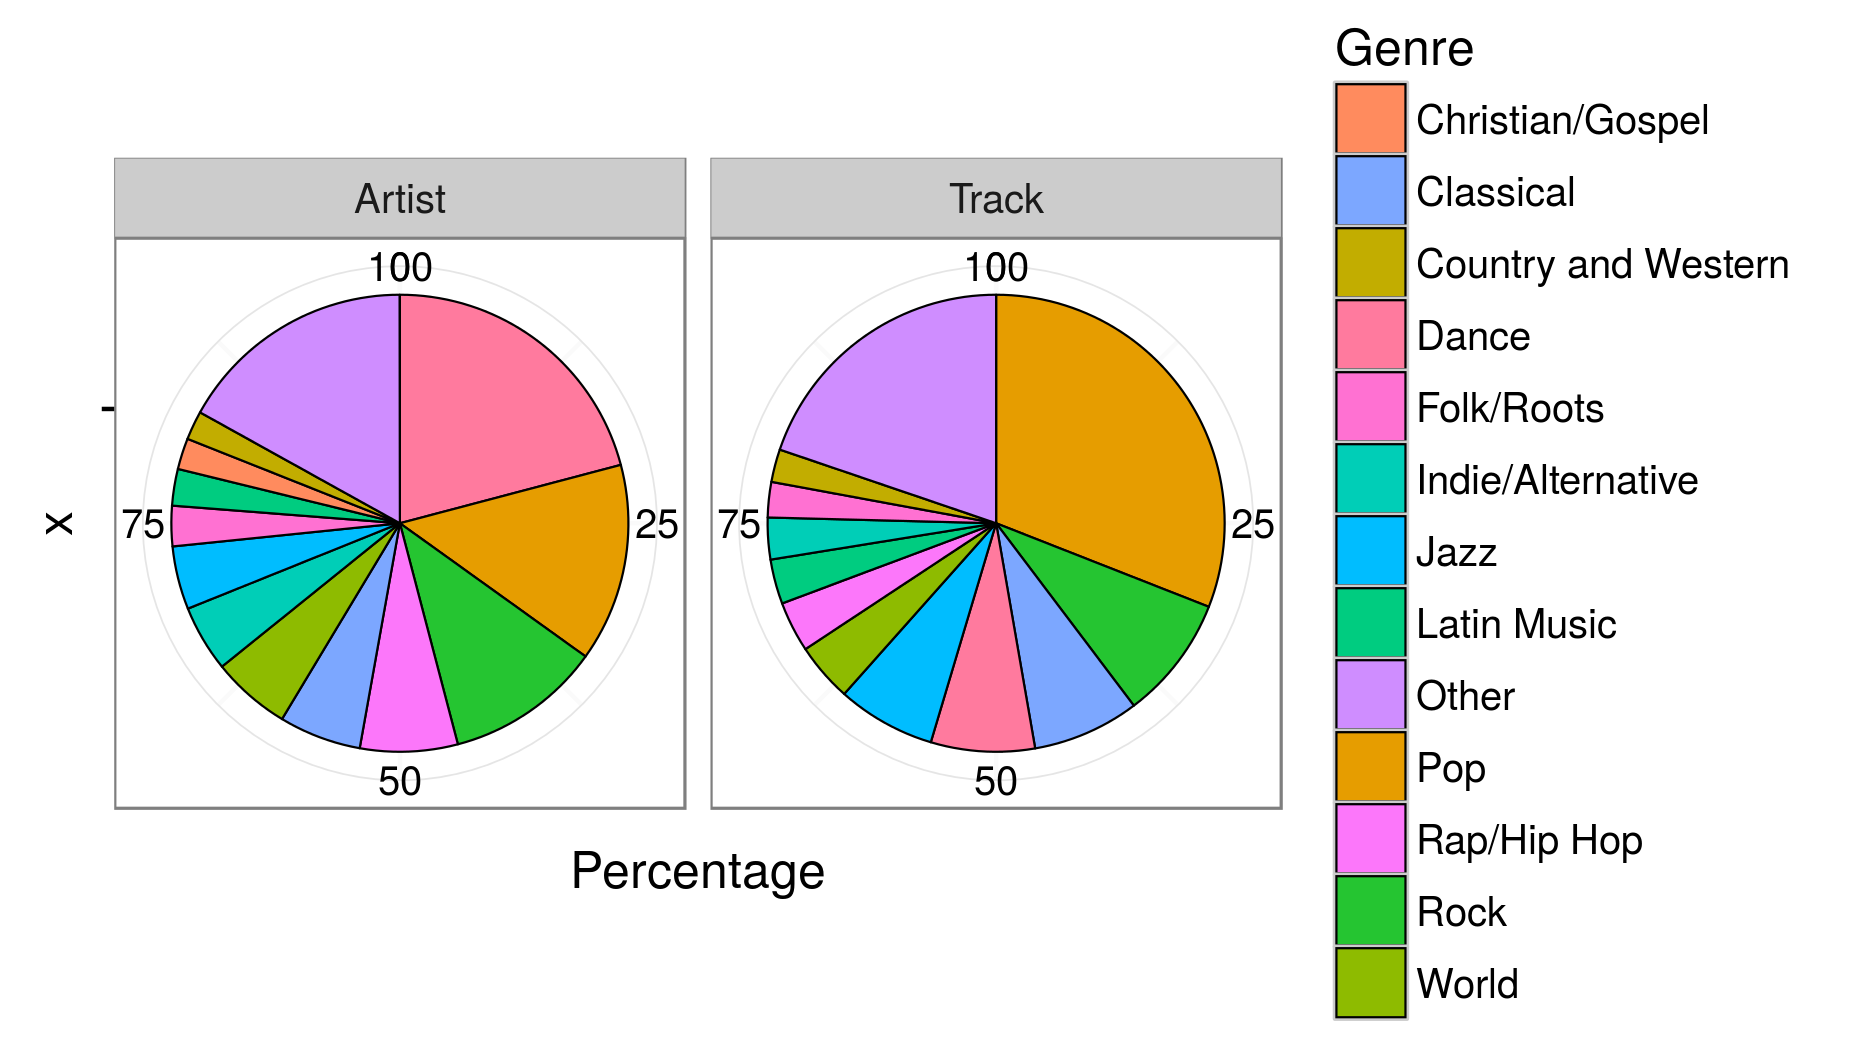
\includegraphics[width=\linewidth]{cataloguePie}
\caption[Track and Artist Genre Distribution]{Percentage of artist and tracks by genre. Dance artists are the most represented artist by genre, and Pop is the most represented track by genre. Genres downloaded < 2\% are aggregated into the "Other" genre}
\label{fig:catpie}
\end{figure}

Preliminary descriptive analyses on total tracks and artists by genre indicate differences in production patterns by content creators.  Total number of artists and tracks grouped by genre were counted and converted to proportions; Figure \ref{fig:catpie} shows the top 10 artists and tracks attributed to a genre in the catalogue. The tenth category, Other, comprises all 53 other genre categories. The majority of tracks in the Nokia DB are Pop, but the majority of artists are Dance suggesting that artists with different genre affiliations release different amounts of tracks.

\begin{figure}[h!]
%Zipf was set to s=.4
\centering
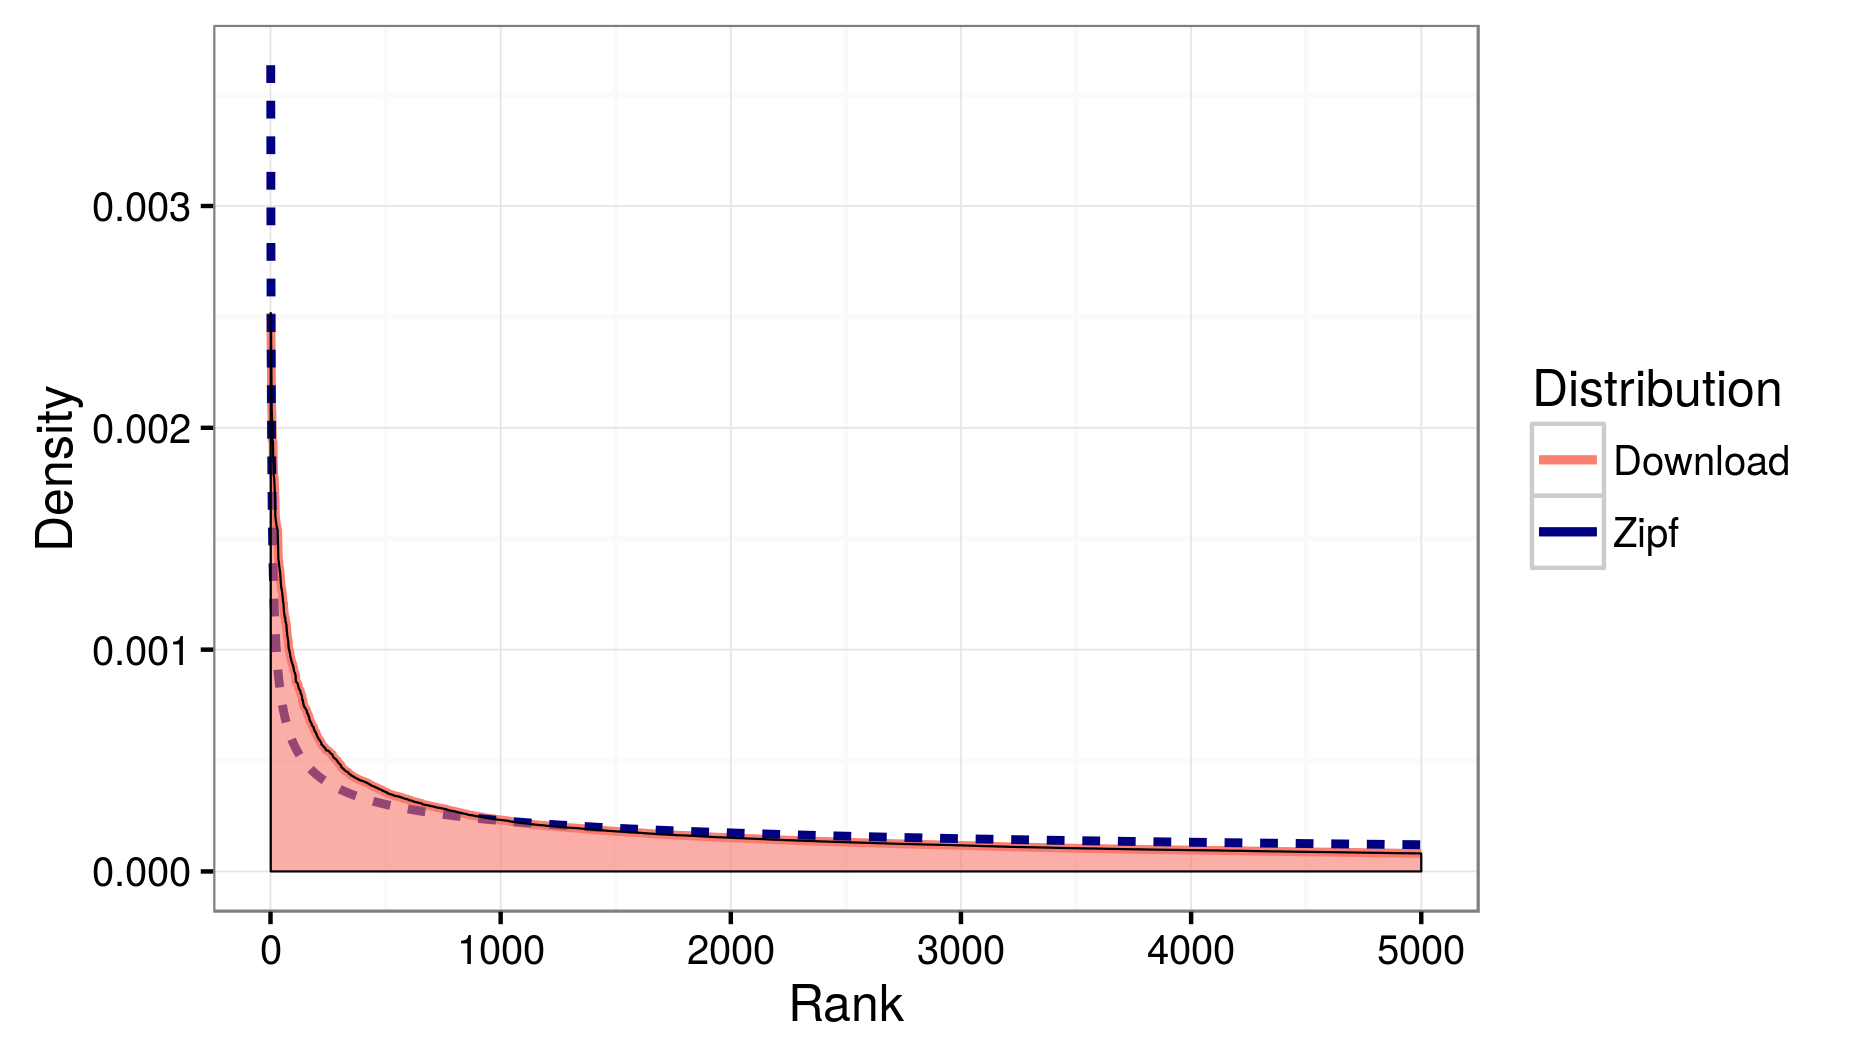
\includegraphics[width=\linewidth]{zipfTrack}
\caption[Zipf distribution and track downloads]{Zipf density distribution and total downloads}
\label{fig:zipf}
\end{figure}

Next, artists were ranked according to their total download count. Figure \ref{fig:zipf} displays the top 5000 most downloaded tracks in the Nokia DB, converted to a proportion (y-axis) and ordered by rank (x-axis). The distribution of music downloads ranked by artist is highly skewed to the most popular performers, and is consistent with research from data provided by other digital services \cite{anderson2007long,levy2010music}. Qualitatively (and represented as a dashed line in Figure \ref{fig:zipf}), the shape of this relationship is similar to a Zipf distribution \cite{wilson1949human}. Zipf distributions have been found with respect to music classification, physiological responses, aesthetics, and acoustic feature extraction \cite{manaris2005zipf,tzanetakis2011music}. To the author's knowledge, no research within MIR or music cognition has demonstrated a Zipf distribution in music with respect to consumption.

Nokia Music's service developed over time, and as a result, all 33 regions did not enter into the database simultaneously. The service first opened in the Great Britain in September 2007, with Venezuela joining the service last in September 2013. Figures \ref{fig:nokiamap07} and \ref{fig:nokiamap14} are global heat maps, coloured by the amount of yearly downloads for each region. Total downloads are normalized by taking the $\log$ of the yearly count in order to visually discern differences in activity. China, India, Finland, Great Britain and Brazil were the most active regions using the service.

\begin{figure}[h!]
\centering
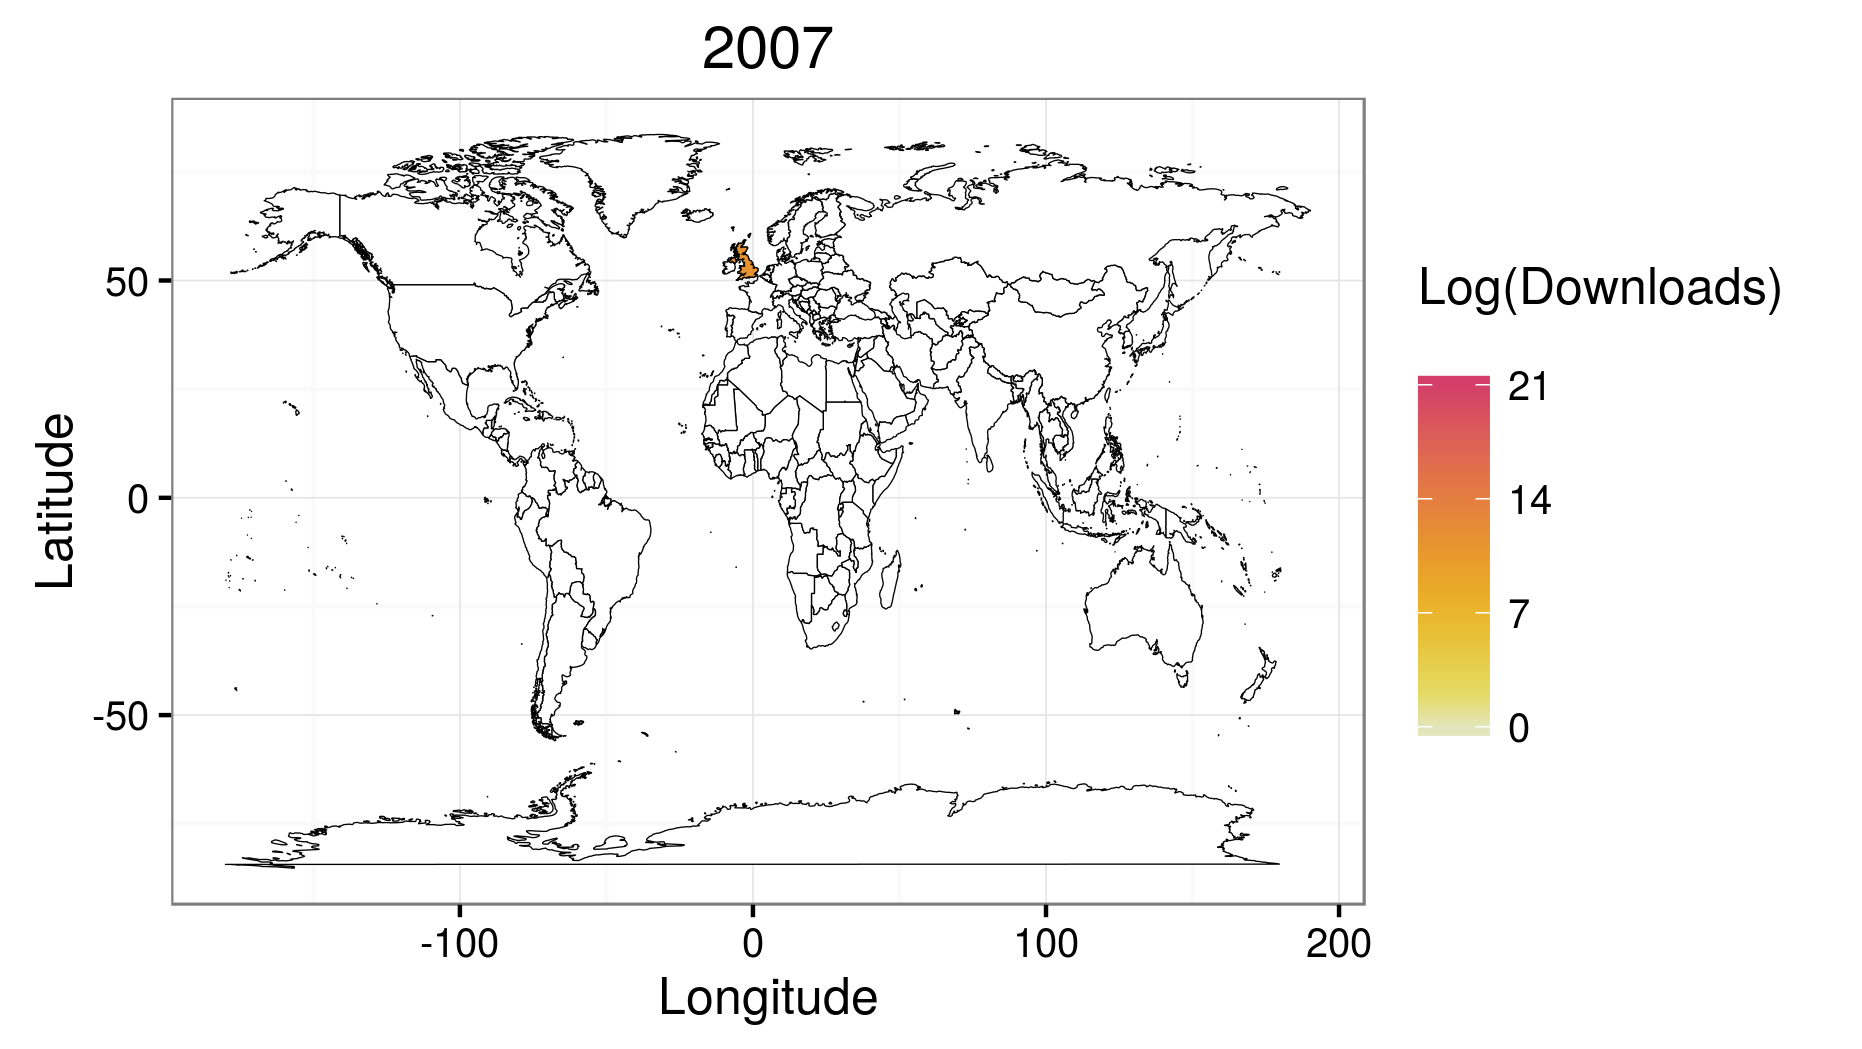
\includegraphics[width=\linewidth]{nokiaMap07}
\caption[Nokia Consumption Map - 2007]{Nokia Consumption Map 2008. Colour intensity illustrate total downloads by country in 2007. Values are converted to $\log$ for scaling}
\label{fig:nokiamap07}
\end{figure}

\begin{figure}[h!]
\centering
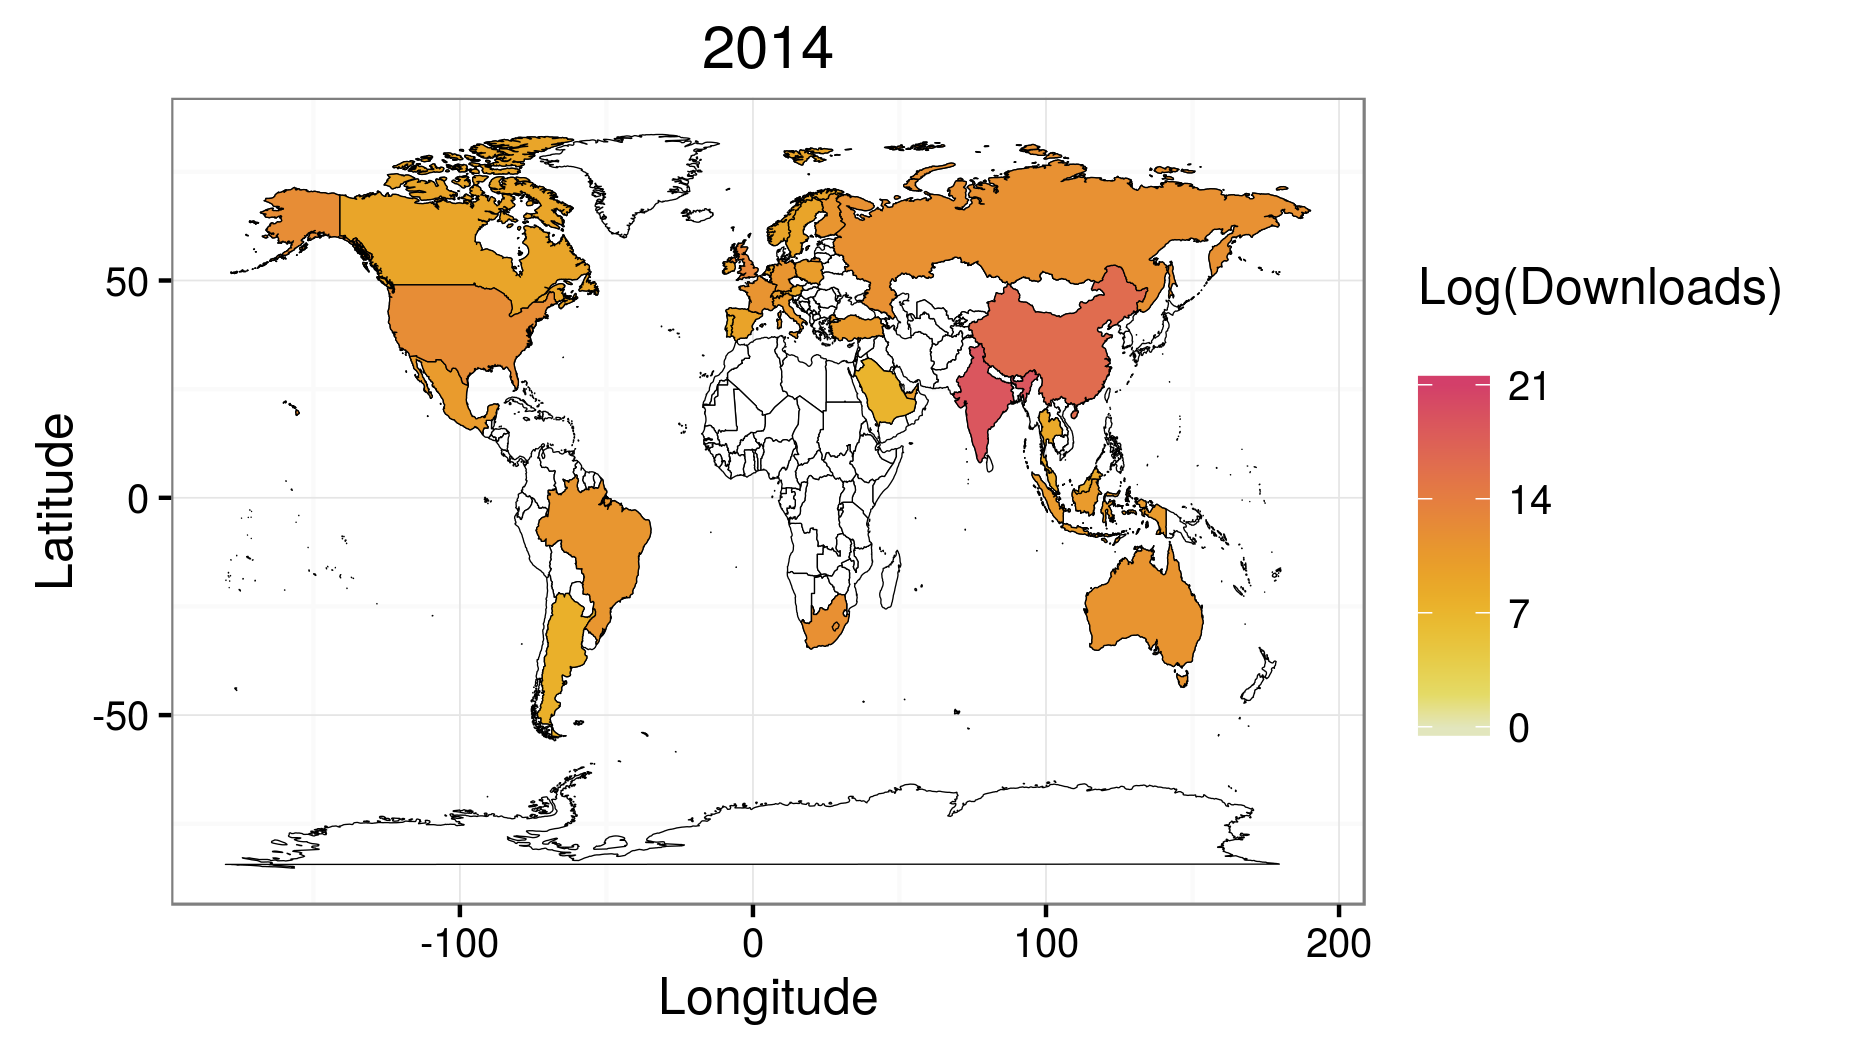
\includegraphics[width=\linewidth]{nokiaMap14}
\caption[Nokia Consumption Map - 2014]{Nokia Consumption Map 2014. Colour intensity illustrate total downloads by country in 2008. Values are converted to $\log$ for scaling}
\label{fig:nokiamap14}
\end{figure}

Of the ca. 36 million tracks available in the Nokia DB catalogue, 9,036,675 tracks were enriched with high-level acoustic features extracted through a variety of signal processing techniques \cite{bogdanov2013essentia,Bogdanov2009FromMeasures}, and musicological information annotated by community driven open-access resources including: MusicBrainz \cite{swartz2002musicbrainz,vigliensoni:00,porter2015acousticbrainz}\footnote{\url{https://musicbrainz.org/}}, Spotify,\footnote{\url{https://www.spotify.com}} and The Echo Nest,\footnote{\url{https://the.echonest.com/}}. In the context of this work, high-level features (i.e. Danceability) refer to a single value derived from an entire track, whereas low-level features (i.e. Mel frequency cepstral coefficients) are arrays of values extracted over small windows (typically seconds) of time.  High-level acoustic features utilized in this thesis include:

\begin{description}\itemsep0em 
\item[Acousticness.] Value representing the probability that a track was created using acoustic instruments, including voice. Float; range, 0-1.
\item[Danceability.] A track’s “foot-tapping” quality, based on tempo, rhythm stability, beat strength and isochrony. Float; range, 0-1.
\item[Duration.] The duration of a track in seconds as calculated by the Spotify analyzer. Float; maximum value, 6060 seconds.
\item[Energy.] A perceptual estimation of frenetic activity throughout a track. High-energy tracks have increased entropy, and tend to feel fast, loud, and noisy (e.g. Death Metal). Float; range, 0-1.
\item[Instrumentalness.] Value representing the probability that a track was created using only instrumental sounds, as opposed to speech and/or singing. Float; range, 0-1.
\item[Liveness.] Value representing the probability that a track was recorded in the presence of an audience rather than in a studio. Float; range, 0-1. 
\item[Loudness.] The average loudness of a track in decibels. Loudness is the psychological correlate of signal amplitude. 
\item[Speechiness.] Value representing the presence of spoken words in a track, e.g. talk show, audio book, poetry, rap. Float; range, 0-1.
\item[Tempo.] The estimated tempo of a track in beats per minute. Float; range, 0-294.
\item[Valence.] A perceptual estimation of a tracks positive/negative affect, e.g. happy and cheerful, or sad and depressed. Float; range, 0-1.
\end{description}

Enrichment was made possible through a metadata linkage, storage, and sharing process created for this thesis known as the General Recorded Audio Identity Linker (\Gls{GRAIL}). \Gls{GRAIL} represents a significant contribution to CogMIR-related research, and is utilized for all analyses in this thesis. Motivations, linking process, and coverage are now outlined. 

\subsection{The General Recorded Audio Identity Linker (GRAIL) \label{sec:grail}}
\subsubsection{Motivation}
Inconsistent music metadata is not merely an esoteric problem for MIR. As of 2012, 42\% of music classification algorithms use open-access data \cite{sturm2012survey}, but resources that verify data accuracy and publish linked music \Gls{API} IDs have been absent from the field. This is important because using a variety of open-access databases for research could be advantageous, but rarely discussed because linking metadata is a complex problem. For example, \cite{angeles:00} attempts to link metadata to the Codaich Database\footnote{\url{http://jmir.sourceforge.net/manuals/jMusicMetaManager_manual/introduction.html}} and found exact matches for only 22\% of popular songs and 0\% for classical. \cite{bogdanov2016cross} using the same classification algorithm across five standard collections found genre identification accuracy to range widely from 48-87\%, reflecting significant differences in music metadata. \cite{corthaut2008connecting} supports the notion of a metadata linking resource, stating that it should, ``...be aware of the existence of different schemas to store and exchange music metadata''. 

Due to services optimizing their data architectures for specific purposes, there is a paucity of consistent music metadata within both academia and industry \cite{corthaut2008connecting}. Metadata faults can be further compounded by incomplete or inconsistent data management practices \cite{angeles:00}, and, in part, to the changing availability of data over time. For example, approximately 50\% of the Million Song Dataset's \cite{bertin:00} linkages to The Echo Nest were no longer accessible immediately prior to its deprecation in 2014,\footnote{\url{https://techcrunch.com/2014/03/07/spotify-echo-nest-100m/}} due to the former service not being consistently updated. Arguably, therefore, in order to reduce data inaccuracies that may accrue over time, it is important for MIR to develop systems that automatically cross-validate, check, and update information from multiple resources.

In order to address these issues, a modular linking system capable of being augmented at any time to access services is utilized. Furthermore, the architecture constantly re-validates music information accuracy, and can store results in a relational database system for later use. A resource of linked IDs from digital music services is valuable for MIR for the following reasons: (1) it can support historic research efforts by linking data collected from deprecated services (e.g. Rdio) to operational ones (e.g. Spotify); (2) new research is enabled by linking data from ontologically distinct resources (e.g. IDs for lyric analysis linked to IDs with consumption information \cite{mckay2010evaluating}); and (3) provide a public resource for cross-validation of metadata provided by music services.\footnote{\url{https://www.berklee.edu/news/fair_music_report}} This work addresses the complex challenges of music-metadata organization, referred to above, and provides our solution in the form of an public \Gls{API}. To the author's knowledge, \Gls{GRAIL} is the only public resource which includes data integrity metrics across multiple resources.

\subsubsection{Web-Crawlers and Workflow}
\begin{figure}[h!]
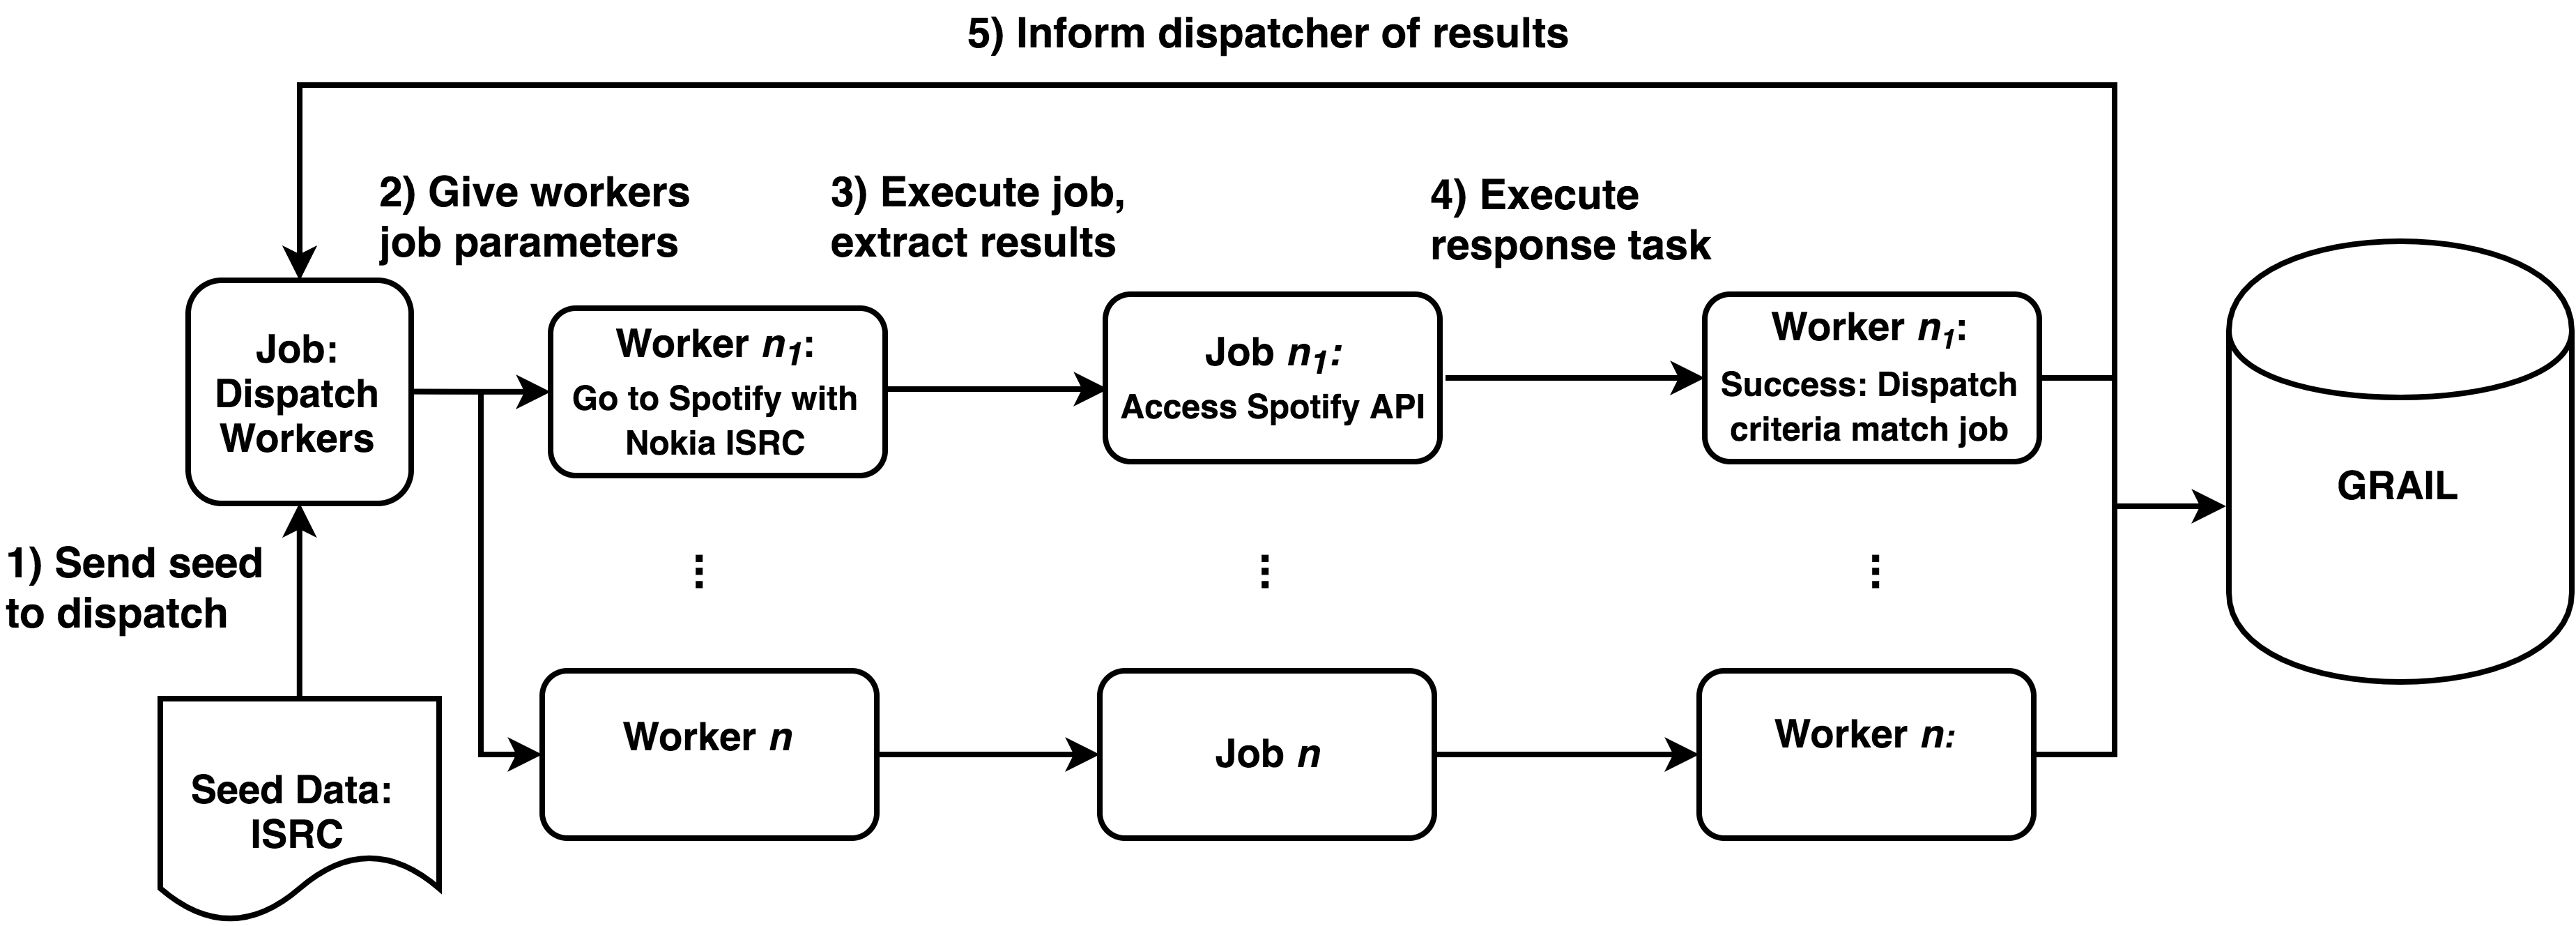
\includegraphics[width=\linewidth]{crawler_workflow.png}
\caption[\Gls{GRAIL} Crawler Process]{Web crawler process. Workers are provided seed-data including necessary \Gls{API} endpoints, validation procedure, and any necessary data required to execute linkages. Workers access an \Gls{API}, conduct the validation procedure, and update \Gls{GRAIL}'s database with new information.}
\label{fig:crawl_process}
\end{figure}

To constantly check and validate \Gls{API} metadata, we developed a web-crawler\footnote{\url{www.github.com/digitalmusiclab/\Gls{GRAIL}_web_crawler}} that asynchronously checks metadata, collects and updates IDs, and cross-validates information from strong linkages to test for data inconsistencies. Figure \ref{fig:crawl_workflow} illustrates a web-crawler job sent to the Spotify \Gls{API}. For this crawl, the scheduler is seeded with Nokia Music metadata, including artist, release, and track information (1). The scheduler spawns a worker, and provides endpoint parameters to crawl Spotify's \Gls{API} (2); e.g. rate-limit restrictions, and what criteria will be employed). The worker executes its task and calculates consistency values (3) (see Section \ref{sec:crit} for validation process). Linked IDs from responses are ingested into \Gls{GRAIL}, alongside calculated consistency values (\Gls{CV}) and timestamp information (4). Lastly, the worker updates \Gls{GRAIL} with job results, and seeds the scheduler with any new information that requires validation based on these results (5). As the crawler verifies any metadata changes, the \Gls{CV}s of the linkages are updated. Some services, such as The Echo Nest, provided additional \Gls{API} IDs; when available, these IDs are also ingested into \Gls{GRAIL} after calculation of consistency. 

\subsubsection{Consistency Analysis}\label{sec:crit}
The metadata linkage analysis is based on three criteria: cardinality ($C$); string-matching ($SM$); and position ($P$). Using these criteria, \Gls{CV}s ($\Gls{C_{CV}}$, $\Gls{SM_{CV}}$, and $\Gls{P_{CV}}$) ranging from zero to one are calculated for artist, release and track IDs. An overall, summary statistic ($\Gls{O_{CV}}$) is also calculated as a weighted average of $\Gls{C_{CV}}$, $\Gls{SM_{CV}}$, and $\Gls{P_{CV}}$. As \Gls{API}s do not offer a universal set of metadata or search methods, it is not always possible for every criterion to be used at every comparison level.\footnote{For example, some \Gls{API}s (e.g. Last.FM, MusixMatch) do not provide track position metadata.} Table \ref{tab:crit} illustrates the criteria ideally used. In the interests of transparency, documentation regarding which criteria are utilized for each \Gls{API} are provided on the \Gls{GRAIL} website.\footnote{\url{api.digitalmusiclab.org}} Information will continue to be updated as \Gls{GRAIL} expands to include other services. Table \ref{tab:release} provides a release analysis between two hypothetical albums.

\begin{table}[ht]
\large
 \begin{center}
 \begin{tabular}{|c||c|c|c|}
  \hline
\textbf{\Gls{CV}} & \textbf{Artist} & \textbf{Release} & \textbf{Track} \\
\hline
\bm{$SM_{CV}$} & \checkmark & \checkmark & \checkmark \\
\bm{$C_{CV}$} & \checkmark & \checkmark & --- \\
\bm{$P_{CV}$} & --- & \checkmark & \checkmark \\ 
\hline
\hline
\bm{$O_{CV}$} & \checkmark & \checkmark & \checkmark \\
\hline
\end{tabular}
\end{center}
  \caption[Criteria Matching Table]{Table showing \Gls{CV}s calculated for artist, release, and track. Overall \Gls{CV}s ($\Gls{O_{CV}}$) are calculated for each level based on a weighted average.}
\label{tab:crit}
\end{table}
\newpage

\begin{table*}[t!]
\centering
\begin{tabular}{|c|c|c|c|c|c|}
  \hline
\textbf{Order} & \textbf{X Release} & \textbf{Y Release} & \bm{$SM_{\Gls{CV}}$} & \bm{$C_{\Gls{CV}}$}   & \bm{$P_{\Gls{CV}}$}  \\
  \hline
\textbf{1.} & im ahab & I am aahb & 0.75 & 0.8 & 1.0 \\
%  \hline
\textbf{2.} & Island & Blood and thunder & 1.0 & 0.8 & 0.6  \\
%  \hline
\textbf{3.} & Sea beast & seabeast & 0.94 & 0.8 & 1.0 \\
% \hline
\textbf{4.} & blood \& thunder & Island & 0.875 & 0.8  & 0.6  \\
\textbf{5.} & Iron tusk & --- & 0.38 & 0.8  & 0.6\\
\hline
\end{tabular}
\caption[Release Criteria Example]{Example of release matching process using two APIs X and Y (e.g. Spotify and MusicBrainz). Release and artist names are first compared prior to assigning track consistency values. When releases agree on artist and release strings, track information regarding the releases is compared. In this example, the 3 columns on the left disagree in the following ways: X has a cardinality of 5, whereas Y's cardinality is 4; and track orders 2 and 4 within X are reversed within Y. The 3 columns on the right show CVs calculated per track for each criterion ($\Gls{C_{CV}}$, $\Gls{SM_{CV}}$ and $\Gls{P_{CV}}$, described below).}
\label{tab:release}
\end{table*}

\paragraph{String-Matching Consistency Value ($\Gls{SM_{CV}}$).}
Levenshtein distances (\Gls{LD}s) \cite{navarro2001guided} are calculated as ratios for tracks, releases, and artists. \Gls{LD} compares character similarity across two strings and provides a value ranging from 0 to 1. LD is a common procedure in string-matching processes, and has been used previously to link music metadata into MusicBrainz\cite{vigliensoni:00}. Track, release, and artist \Gls{LD}s are calculated on a pairwise basis, and expressed as $\Gls{SM_{CV}}$ values (see Table \ref{tab:release}, Column 4). For example, in Table \ref{tab:release} the 3rd track under X is "Sea Beast"; whereas under Y it is "seabeast", resulting in a \Gls{LD}/$SM_{CV}$ of $0.94$.

\paragraph{Cardinality Consistency Value ($\Gls{C_{CV}}$).}
$\Gls{C_{CV}}$ values are calculated by dividing the minimum cardinality by the maximum; see Equation \ref{eq:card}. For example, Table \ref{tab:release} compares two releases, X and Y, with different cardinalities (5 versus 4). The $\Gls{C_{CV}}$ column in Table \ref{tab:release} (Column 5) is therefore: $\frac{4}{5}=0.8$. This value is attributed to each track within both releases. In a similar manner, artist-level cardinality is calculated by comparing the number of distinct tracks attributed to each artist across resources. As Table \ref{tab:crit} shows, the cardinality criterion is not used with respect to track matching.

\begin{equation}
C_{CV} (X,Y) =  \frac{C \min}{C \max}
\label{eq:card}
\end{equation}
\myequations{Cardinality}

\paragraph{Position Consistency Value ($\Gls{P_{CV}}$).}
When position metadata are available, $\Gls{P_{CV}}$ is calculated for tracks and releases. Similar to the $\Gls{C_{CV}}$, $\Gls{P_{CV}}$ is calculated for the track with the maximum \Gls{LD} comparison; the linked attribute from the \Gls{API} with the maximum position is used as the denominator against the attribute with the minimum position; see Equation \ref{eq:position}. In Table \ref{tab:release}, Track 2 in X is to Track 4 in Y, the strings exactly match. The $\Gls{P_{CV}}$ for Track 2 in X is therefore $0.6$, calculated by dividing the minimum track position ($2$) by the maximum ($4$).

\begin{equation}
P_{CV} (X,Y) =  1 - \frac{ |X_{Order} - Y_{Order}|}{C \max}
\label{eq:position}
\end{equation}

\paragraph{Overall Consistency Value ($\Gls{O_{CV}}$).}
$\Gls{O_{CV}}$ values are calculated for artist, release and track by taking a weighted average from all available \Gls{CV}s. As shown in Table \ref{tab:crit} Artist $\Gls{O_{CV}}$s are calculated by taking the weighted average of $\Gls{SM_{CV}}$ and $\Gls{C_{CV}}$; track $\Gls{O_{CV}}$s are calculated by taking the weighted average of $\Gls{SM_{CV}}$ and $\Gls{P_{CV}}$. For a release $\Gls{O_{CV}}$, a weighted average of all \Gls{CV}s is possible. Using the example in Table \ref{tab:release}, the overall release score for this comparison would be: $\mu (\Gls{SM_{CV}},\Gls{P_{CV}},\Gls{C_{CV}})$.

\begin{figure}[h!]
\centering
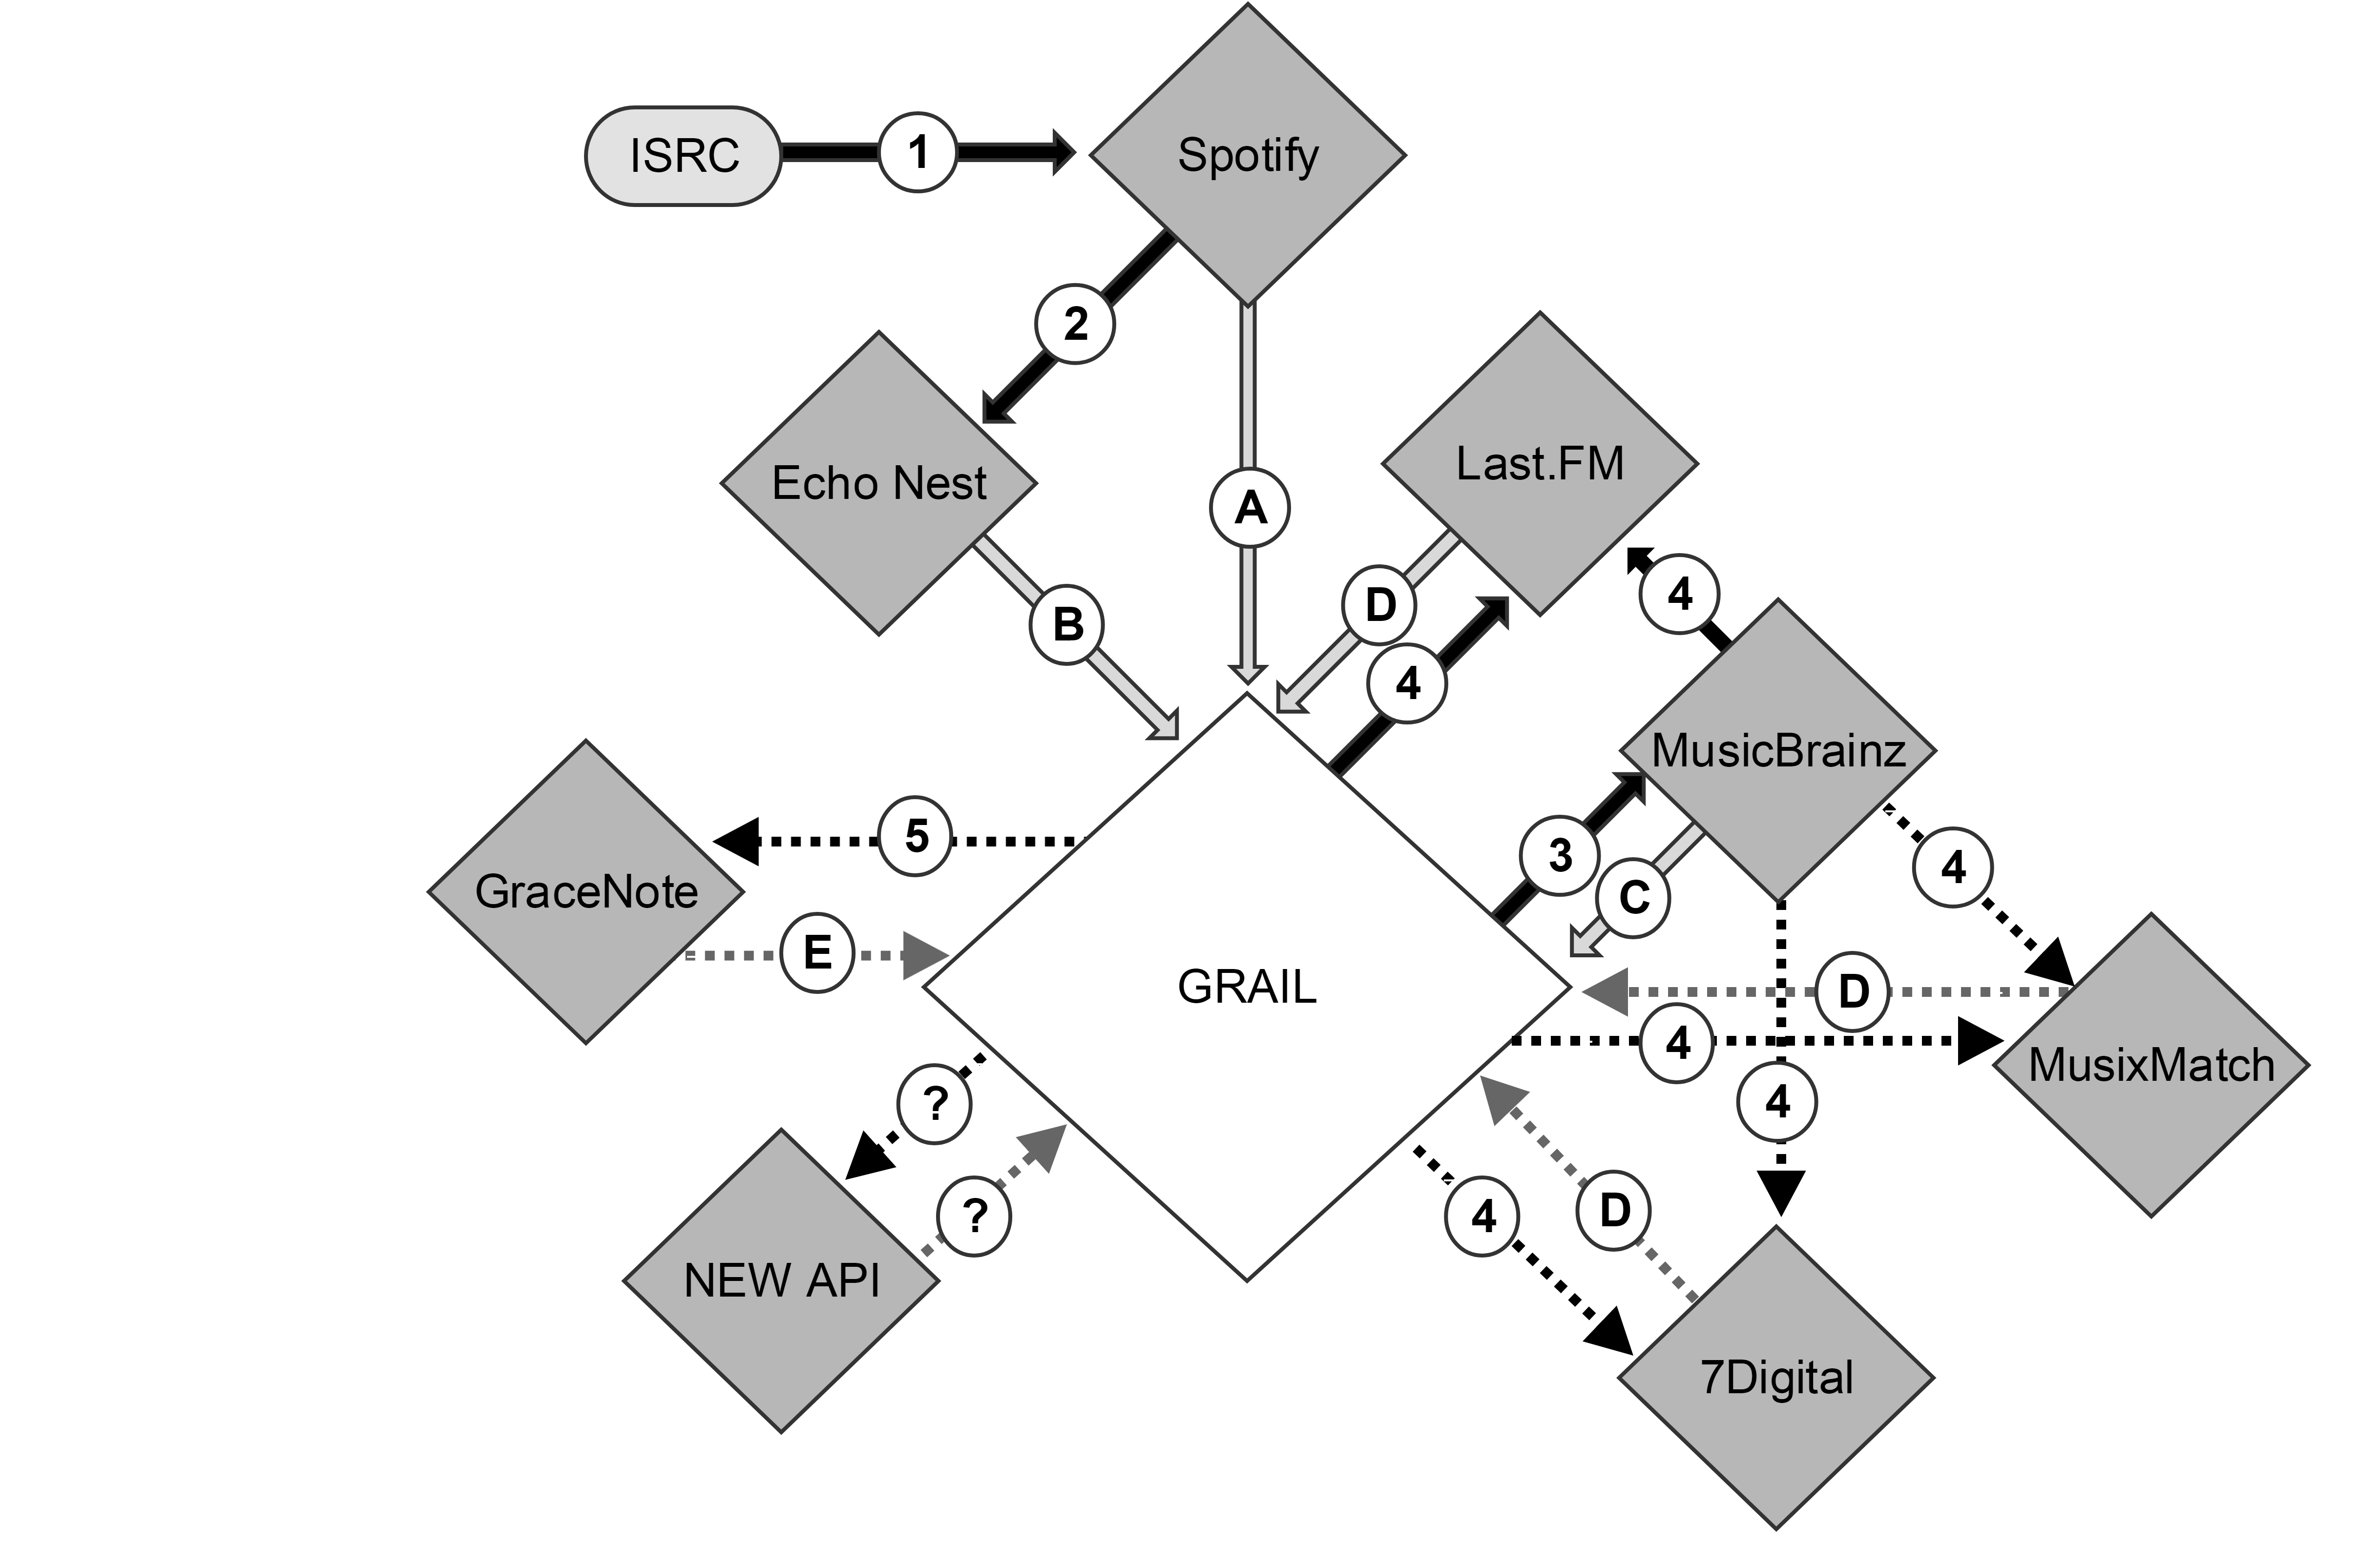
\includegraphics[width=\linewidth]{grail_workflow.png}
\caption[\Gls{GRAIL} Crawler Workflow]{Workflow llustrates how crawlers access targeted \Gls{API}s (gray diamonds), what validation steps are used to access \Gls{API}s (black lines), and what metadata is ingested into \Gls{GRAIL} (gray lines). Solid lines represent active \Gls{GRAIL} crawls, and dotted lines represent crawls currently in development.}
\label{fig:crawl_workflow}
\end{figure}

\bigskip

Figure \ref{fig:crawl_workflow} is a schematic representation of \Gls{GRAIL}, and the way in which jobs are processed and information is ingested. Jobs are separated into validation steps (numeric circles) and ingestion steps (letter circles), and are described below:\\

\paragraph{Validation Steps}
\begin{description}\itemsep0em 
\item[Step 1.] International Standard Recording Code (\Gls{ISRC}) seed-data from Nokia DB accesses metadata from the Spotify \Gls{API}. Artist, release, and track consistency calculations are conducted using $\Gls{SM_{CV}}$, $\Gls{P_{CV}}$, and $\Gls{C_{CV}}$.
\item[Step 2.] Spotify tracks IDs were used to link to Rosetta Stone artist IDs.\footnote{\url{https://musicmachinery.com/2010/02/10/introducing-project-rosetta-stone/}} Due to Spotify's purchase of The Echo Nest in 2014 and subsequent discontinuation, consistency validation between this two services was not possible (or necessary).
\item[Step 3.] Nokia Music artist, release, and track string names are used to query the MusicBrainz \Gls{API}.  Artist, release, and track consistency calculation using $\Gls{SM_{CV}}$, $\Gls{P_{CV}}$, and $\Gls{C_{CV}}$.
\item[Step 4.] Nokia Music artist, release and track string names, and linked MusicBrainz IDs, from ingestion step C are being used to conduct artist, release, and track consistency calculations using $\Gls{SM_{CV}}$, $\Gls{P_{CV}}$, and $\Gls{C_{CV}}$.
\item[Step 5.] In due course, Nokia Music artist, release, track string names will be used to access GraceNote's metadata via text search. As above, artist, release, and track consistency calculations are conducted using $\Gls{SM_{CV}}$, $\Gls{P_{CV}}$, and $\Gls{C_{CV}}$.
\end{description}

\paragraph{Ingestion Steps}
\begin{description}\itemsep0em 
\item[Step A.] Spotify artist, release, and track IDs are ingested into \Gls{GRAIL}. Crawlers check if an ID has changed since last checked. New IDs, including CV values and timestamps, are inserted as additional rows. IDs which have not changed are updated with modified CV values and timestamps.
\item[Step B.] The Echo Nest track and artist IDs were ingested into \Gls{GRAIL}, in addition to any artist IDs collected from the Rosetta Stone project.
\item[Step C.] MusicBrainz artist, release, and track IDs are ingested into \Gls{GRAIL} based on \Gls{API} text searches.
\item[Step D.] Artist, release, and track IDs CVs are calculated for Last.FM metadata, and are ingested to \Gls{GRAIL} using linked MusicBrainz IDs and text searches. MusixMatch and 7digital \Gls{API} crawlers are in development using a similar process.
\item[Step E.] Artist, release, and track ID CVs will be ingested for new \Gls{API}s, and any shared metadata that can improve accuracy.
\end{description}

Each API validation conducts consistency analyses using all available metadata shared between resources. As discussed in Section \ref{sec:grail}, resources are not consistent with respect to the information they provide and how it can be accessed. To that end, linkage processes across APIs have different dependencies. For instance, Spotify's coverage of \Gls{ISRC}s are more extensive than in MusicBrainz, track-level requests are made to Spotify first, followed by release- and artist- validation. Whereas in MusicBrainz, the most comprehensive request we can make is at the release-level first, followed by track and artist.

\subsubsection{Linkage Results}
Table \ref{tab:results} describes the outcome of our linkages to date. In summary, we have ingested millions of IDs from 16 providers at track, release, and artist levels into \Gls{GRAIL}, making it, to our knowledge, possibly the largest set of linked metadata of its type available for public use. Spotify achieves the highest linkage results, because the \Gls{API} can be queried with \Gls{ISRC}s, of which there are a 12 million distinct examples within \Gls{GRAIL}. Given the ongoing activity of the crawlers, we anticipate that the numbers in Table \ref{tab:results}, both in terms of linkages and services will expand significantly, other than those services which are discontinued (Table \ref{tab:results}, asterisks).

\begin{table}
\centering
\begin{tabular}{|l|c|}
\hline
\textbf{API ID Space} & \textbf{No. Linkages}  \\
\hline
Spotify track IDs & 17.5M  \\
Nokia Music track ID* & 11.8M \\
Echo Nest track ID*  & 6.5M  \\
MusicBrainz track ID & 465K  \\
MSD track ID & 521K  \\
MusixMatch track ID & 3.8M \\
LyricFind track ID & 1.5M  \\
\hline
Spotify release ID & 1.5M  \\
Nokia Music release ID*  & 1.6M \\
MusicBrainz release ID & 523K  \\ 
\hline
Spotify artist ID & 6.6M  \\
Nokia Music artist ID* & 358K \\
MusicBrainz artist ID & 203K  \\
MusixMatch artist ID & 2.1M  \\
Jambase artist ID & 860K  \\
OpenAura artist ID & 3.7M  \\
SeatGeek artist ID & 2.8M  \\
Seatwave artist ID & 740K  \\
LyricFind artist ID & 1.5M  \\
Twitter artist ID & 670K  \\
Facebook artist ID & 3.7M  \\
Tumblr artist ID & 27K  \\
FMA artist ID & 240K  \\
7digital artist ID & 5.5M  \\
\hline
\end{tabular}
\caption[Linkage Results]{\Gls{GRAIL} linkage results for track, release, and artist IDs. Asterisks indicate discontinued services.}
\label{tab:results}
\end{table}

\subsubsection{Application Program Interface}
All \Gls{GRAIL} linkages are provided for public use through the \Gls{GRAIL} REST \Gls{API} (\url{https://api.digitalmusiclab.org/}). Users can query the \Gls{API} using track, release or artist IDs or strings, from a documented list of services and datasets (refer to Figure \ref{tab:results} for resource availability). Users can request specific IDs in return and filter requested IDs based on CV thresholds, and timestamps (e.g. most recent crawl). Updated documentation relating to validation calculations, resource availability, and API news can be accessed via the website. The code for crawlers, website, and \Gls{API} are available on github at: \url{https://github.com/digitalmusiclab/}

\Gls{GRAIL} requires an authentication key in order to be accessed. Authentication keys are generated as part of the free registration process available via the \Gls{GRAIL} website. The terms of service state that this \Gls{API} is for, and by the Creative Commons, designed for use in MIR research. \Gls{API} keys are rate limited based on current server restrictions. Users are restricted from using \Gls{GRAIL} for profit without direct consent from the services within \Gls{GRAIL} and in their applications.

\subsubsection{GRAIL Applications}
Accessible and validated metadata has important uses for the MIR community and can contribute to innovative research. \Gls{GRAIL} could arguably improve top-performing genre-classifiers which use a diverse combination of user behaviour, lyrics, and cultural information \cite{mckay2010evaluating} with expanded datasets. Perhaps more directly, psychological work examining the degree to which acoustic features influence musical choices was made possible through \Gls{GRAIL}'s linkages to open-access resources \cite{barone2017leaky,bansal2015predictive}. Future work using \Gls{GRAIL} may wish to consider exploiting linkages to lyric databases to examine the relationship between sung words and preference using psycholinguistics and computational natural language processing. In sum, accessibility to already linked metadata without having to readdress data validation makes new research more feasible.

Accurate metadata is also vital for the music industry; a study by Berkley University found that between 20--50 percent of music payments from digital services do not reach the rightsholder.\footnote{\url{https://www.berklee.edu/news/fair_music_report}} Community-maintained databases \cite{bertin:00, swartz2002musicbrainz, cannam2010linked} provide essential metadata, and attempt to alleviate some of these challenges. However, the quality of data linkages can degrade over time without constant re-validation, as previously discussed. Furthermore, invaluable open resources like The Echo Nest can suddenly deprecate due to corporate buyouts or insufficient funding, arresting global research and development reliant upon it.\footnote{\url{https://blog.musicbrainz.org/2016/04/01/deprecating-mbids/}} \Gls{GRAIL} may be a valuable resource, in that it addresses the above issues; as the Berkley study suggests, a community-maintained database linked to \Gls{ISRC}s is a necessary step to reduce data faults and improve non-payment of artists, which \Gls{GRAIL}'s linkage process is based on.

Research relevant to this thesis using \Gls{GRAIL} assessing music preference is now discussed. Section \ref{sec:leaky} uses personality and mood research to inform an investigation of user preference and genre using high-level extracted acoustic features provided through \Gls{GRAIL}'s linkage to the Echo Nest; Section \ref{sec:hdi} relies on cross-cultural psychology research as a framework to relate measures of user behaviour metrics such as eclecticism and temporality to \Gls{GRAIL}'s linkage to yearly United Nations human development data pertaining to health, income, and education. Section \ref{sec:future} discusses future applications using \Gls{GRAIL} to refine current analyses and to contribute new areas of research.

\section{Analyses} \label{sec:analyses}
\subsection{Cognitive Influence} \label{sec:leaky}
Similarly to the devices used in our study, which were mobile phones and PCs (see Section \ref{sec:nokia}), \cite{butt2008personality} sought to predict patterns of mobile-phone use from 120 participants' using the Coopersmith self-esteem inventory \cite{coopersmith1981} assessing four of the Big Five personality traits (extraversion, agreeableness, conscientiousness, neuroticism), and self-esteem. Individuals assessed as being neurotic, disagreeable, unconscientious and/or extraverted tended to spend more time messaging using SMS; disagreeable extraverts changed cellphone backgrounds and ringtones more frequently, indicating phone use as a means of stimulation and/or diversion; individuals who scored highly in neuroticism had relatively greater internet use, according to the authors, perhaps in an attempt to overcome loneliness. 

In addition to device- and personality-specific research, studies exploring the interconnectedness of various forms of media and the consumption of culture, including music, have been undertaken. \cite{rentfrow2003re} assert that the perception of a musical genre depends in part upon the social setting in which it is heard and, by extension, the medium through which it is accessed; in other words, that people’s preferences for certain media over others may influence musical categorization. With respect to music listening, personality studies have uncovered multiple associations: openness with Blues and Jazz; conscientiousness with Soul and Funk; extraversion with Pop and Rap, and so on (\cite{zweigenhaft2008re}; see also \cite{rentfrow2003re}). Moreover, personality appears not only to influence the extent to which individual genres are chosen, but also whether we possess narrow or wide-ranging music-listening habits \cite{rawlings1997music}. In sum, personality research provides evidence for the existence of an overarching psychological framework in which effects akin to cognitive leakiness may occur \cite{rieskamp2006extending}. As the research outlined above indicates, personality is a potent phenomenon, suffusing, guiding and shaping our decisions.

While successfully modeling human behavior, some researchers (e.g. \cite{ross2009personality}) have argued that personality traits may be too general to capture the subtle relationship between personality and online behaviour, including cellphone usage. For example, \cite{hughes2012tale} investigated whether a lower-order, relatively narrow personality facet such as Need for Cognition (NFC) was able to predict online social and information-seeking behaviors. NFC is an individual’s predisposition to engage with and enjoy information and cognitive endeavours, e.g. news content, crossword puzzles, Sudoku (\cite{verplanken1993need, haugtvedt1992need}). Despite its specificity, as opposed to a broader dimension such as openness, NFC (in addition to other personality-related factors) in the study conducted by \cite{hughes2012tale} was found to correlate positively with Twitter usage, presumably, due to this social networking service’s relatively high information content. Those with high ratings for sociability and extraversion appeared to prefer Facebook. In sum, \cite{butt2008personality} concluded that psychological profiling with respect to established personality dimensions could robustly explain how people chose to use their mobile phones.

In contrast to personality, which is relatively stable over time \cite{leon1979personality}, mood can undergo rapid affective swings \cite{mcfarlane1988mood}. Moreover, while research has tended to concentrate on how music influences or induces mood, particularly with respect to consumer choice (e.g. \cite{north1999influence, kim1993influence,turley2000atmospheric,areni1993influence}), the converse is also true: mood influences musical choice \cite{friedman2012re}. Which is to say, assuming environmental factors and personal histories to be equal, a person’s musical preferences do not depend solely on their personality, but, in addition, are subject to spur-of-the-moment choices influenced by mood. Amongst the theoretical models advanced to elucidate the role of mood in decision-making, perhaps the most influential is the Affect Infusion Model (AIM) \cite{forgas1995mood}. In brief, the AIM seeks to explain how mood determines a person’s capacity to process information—the importance of mood tends to increase in situations involving heavy cognitive load. As information complexity rises, and redundancy falls, the influence of mood on an individual’s evaluations and responses increases, resulting in “intuitive” decision-making. Arguably, therefore, when faced with a plethora of diverse musical artists, tracks and genres, people tend to rely more upon their current mood, in which case the influence of personality may be temporarily reduced or suspended. To the author's knowledge, within the domain of music-preference research, this hypothesis has yet to be directly tested. 

Despite this possible lacuna within the experimental literature, paradigms employing music-induced moods have produced results that are consistent with aspects of the AIM model. For example, risk-taking varies when mood is induced through listening to preferred versus disliked music. In a real-money gambling study, in which participants placed bets during either music-liked or disliked trial blocks, \cite{halko2015risk} found that people’s appetites for risk-taking significantly increased when listening to preferred tracks. They conjectured that listening to preferred types of music increases the “marginal utility” of money (i.e. the additional satisfaction someone gains from consuming a good or service; \cite{kauder2015history,turley2000atmospheric,areni1993influence}), which, in turn, increases the likelihood of participating in gambling. Although the foregoing covers aspects of decision-making involving music, none of the research and experimental scenarios referred to above necessarily replicate or are fully applicable to the particular issue at hand; namely, the degree to which the features of a person’s preferred musical genre influence their choice of tracks or how musical tastes in the other genres they choose to consume. That personality and/or mood are in part responsible for why certain tracks belonging to different genres are preferred would seem to be self-evident—personality and mood underscore multiple aspects of human behavior, and presumably also our musical choices within genres of secondary importance. However, the extent to which personality and/or mood influence secondary musical choices is opaque. Supported by mood, personality, and statistical learning research, Section \ref{sec:leaky} explores the dynamics of musical preference using extracted acoustic features using Nokia's digital music streaming service (see Section \ref{sec:nokia} for detailed description of data).

This topic is divided into three main analyses. Using correlation, Section \ref{sec:leaky_anal_1} identified differences in feature-dispersion patterns of genre defined subgroups of users. Section \ref{sec:leaky_anal_2} 2 involved the exhaustive calculation of feature-influence matrices, which, in combination with central-tendency statistics, were used to detect the influence of main-genre features on those of secondary genres. Lastly, Section \ref{sec:leaky_anal_3} investigated whether users whose main genre strongly dominated their collections exhibited a greater degree of feature influence with respect to secondary genres in comparison to users with relatively heterogeneous collections. Results strongly indicated that specific acoustic features in users’ main genres influence the music they listened to when downloading secondary genres; the intensity of this influence appears to be related to the strength of preference for the main genre.

\subsubsection{Users as "X-heads"}\label{sec:xhead}
Due to the anonymous and sparse demographic information regarding our users, the behavioural aspect of our analyses are primarily based on the categorization of users into “X-head” subgroups, where X is the most numerous genre in their song download history. For example, a user with a majority of Metal downloads was classified as a Metal-head; most Classical downloads, a Classical-head and so on.\footnote{In rare instances where no genre had an absolute majority, the chronologically earliest downloaded genre is used to determine the user’s categorization.}

An additional consequence of this categorization is the ability to determine the relative strength of a user's preference for a particular genre. We calculate a user's general preference for their favourite genre by normalizing their download histories into proportions by genre. For instance, if a user downloaded ten songs with six of the downloads labelled as Jazz, they would be classified as a Jazz-head, and the strength of their Jazz-preference is 0.6. 

Calculating this value for every user was aggregated for each X-head subgroup to visualize population distributions for intensity of preference (see Figure \ref{fig:xweightDists} for a 4-genre sample). Comparing distribution statistics enables a high-level comparison of preference strength and characteristics across different X-head subgroups (i.e. in general, which communities are more heterogeneous with respect to the other genres they consume). Users with at least 20 downloads and over 7 days of retention (see Section \ref{sec:nokia}) were selected for analysis.

\subsubsection{Analysis 1: Feature Descriptors}\label{sec:leaky_anal_1}
The initial task in Analysis 1 was to identify whether extracted acoustic features (see Section \ref{sec:grail} for acoustic feature description) for pairs of X-head subgroups are distinct. The reason for this is illustrated in Figures \ref{good_4lines} and \ref{bad_4lines}. Figure \ref{good_4lines} shows the Energy distributions of tracks belonging to two X-head subgroups: the solid-orange line, $D_M$, shows the distribution for Dance tracks downloaded by Dance-heads ($Dance_{\textit{Main}}$ = $D_M$); the solid-blue line, $J_M$, shows the distribution for Jazz tracks downloaded by Jazz-heads ($Jazz_{\textit{Main}}$ = $J_M$). Notice that the peak of $D_M$ is to the right, while the peak of $J_M$ is to the left. The two peaks’ relative positions indicate that, in general, Dance tracks listened to by Dance-heads have higher Energy than Jazz tracks listened to by Jazz-heads, as calculated by the Spotify analyzer. 

Also present within Figure \ref{good_4lines} are lines that show Energy distributions belonging to Dance- and Jazz-heads, but for tracks other than their predominant genres: the dotted-orange line, $D_O$, shows the distribution of non-Dance tracks downloaded by Dance-heads ($Dance_{\textit{Other}}$ = $D_O$); the dotted-blue line, $J_O$, shows the distribution of non-Jazz tracks downloaded by Jazz-heads ($Jazz_{\textit{Other}}$ = $J_O$). Two things are important to note: (1) that the Dance-heads’ non-Dance tracks Energy distribution mirrors the distribution of their Dance tracks, e.g. both $D_M$ and $D_O$ peak on the right; and (2) that the Jazz-heads’ non-Jazz tracks Energy distribution mirrors the distribution of their Jazz tracks, e.g. both $J_M$ and $J_O$ peak on the left. Which is to say, when Dance-heads download non-Dance tracks, there is a tendency for these tracks to be similar in terms of Energy to Dance tracks. Alternatively put, the generally high Energy of Dance tracks influences the choices Dance-heads make with respect to non-Dance music, while the generally low Energy of Jazz tracks influences the choices Jazz-heads make with respect to non-Jazz music. 

The observation above relies upon X-head pairs having dissimilar feature distributions (i.e. lines $D_M$ and $J_M$), and, in the case of Figure \ref{good_4lines}, the distribution of $D_M$ being closer to $D_O$ than $J_O$, and $J_M$ being closer to $J_O$ than $D_O$. If, however, the distributions of the X-heads’ main genres are homologous, as is the case for Bollywood- and Reggae-heads in Figure \ref{bad_4lines} (solid green and purple lines), then no such pattern of similar/different distributions is possible. Which is to say, distributions where X-heads’ main genres are more-or-less similar, are less able to demonstrate musical-feature influence. 

The distributions for all possible X-heads’ main genres were correlated with each other in order to identify pairs with dissimilar distributions. This was conducted for all ten features. Using Pearson product-moment correlation, five features yielded no negative coefficients, and were thereby eliminated from the analysis. The five remaining features yielding negative coefficients, usable in the analysis, included Acousticness, Danceability, Energy, Loudness, and Valence. Figure \ref{energy_corrMat} shows the correlation matrix for feature Energy. The two highlighted cells within the matrix relate to the solid lines in Figures \ref{good_4lines} and \ref{bad_4lines}, Dance and Jazz, and Bollywood and Reggae respectively. The Dance-Jazz coefficient is negative (reflected in the dissimilar distributions in Figure \ref{good_4lines}); the Bollywood-Reggae coefficient is positive (reflected in the similar distributions in Figure \ref{bad_4lines}). In the case of Energy, this process yielded 19 X-head pairs suitable for analysis, i.e. 19 cells with negative coefficients. 

Following this, for each X-head pair AB, the distribution of A’s main genre (e.g. $D_M$, Figure \ref{good_4lines}) was correlated with the distribution of A’s other music (e.g. $D_O$). Next, the distribution of A’s main genre (e.g. $D_M$) was correlated with the distribution of B’s other music (e.g. $J_O$). This produced two coefficients. This process was then repeated for B: B’s main genre (e.g. $J_M$) was correlated with the distribution of their other music (e.g. $J_O$), and the distribution of B’s main genre (e.g. $J_M$) was correlated with the distribution of A’s other music (e.g. $D_O$). A and B together, therefore, produced four coefficients. For each feature, this was repeated for all X-head pairs with negatively correlated distributions, and the resulting coefficients entered into a paired sample t-tests in which “within-group” coefficients (e.g. $D_M$ correlated with $D_O$) were paired with “between-group” coefficients (e.g. $D_M$ correlated with $J_O$). 

Figure \ref{tTest_Outline} illustrates this process for Energy with respect to Dance- and Jazz-heads. In total, the 19 X-head pairs identified in the Energy correlation matrix in Figure \ref{energy_corrMat} gave rise to a t-test into which 38 pairs were entered. This enabled us to observe whether there was a closer relationship between the features of A’s main genre and their other music (Figure \ref{tTest_Outline}, red column; e.g. $D_M$ and $D_O$) than with the features of B’s other music (Figure \ref{tTest_Outline}, blue column; e.g. $D_M$ and $J_O$) and vice versa, i.e. whether there was a significant influence of the main genre on music of secondary importance within people’s downloads. If there had been no influence, then the distributions of either A or B’s other music (i.e. $D_O$ or $J_O$) would not be expected to show a consistently closer relationship to their respective main genre distributions (i.e. $D_M$ or $J_M$). The results of this analysis for the five viable features referred to above are now presented. 

%FIGURE 1
\begin{figure}[h!]
\centering
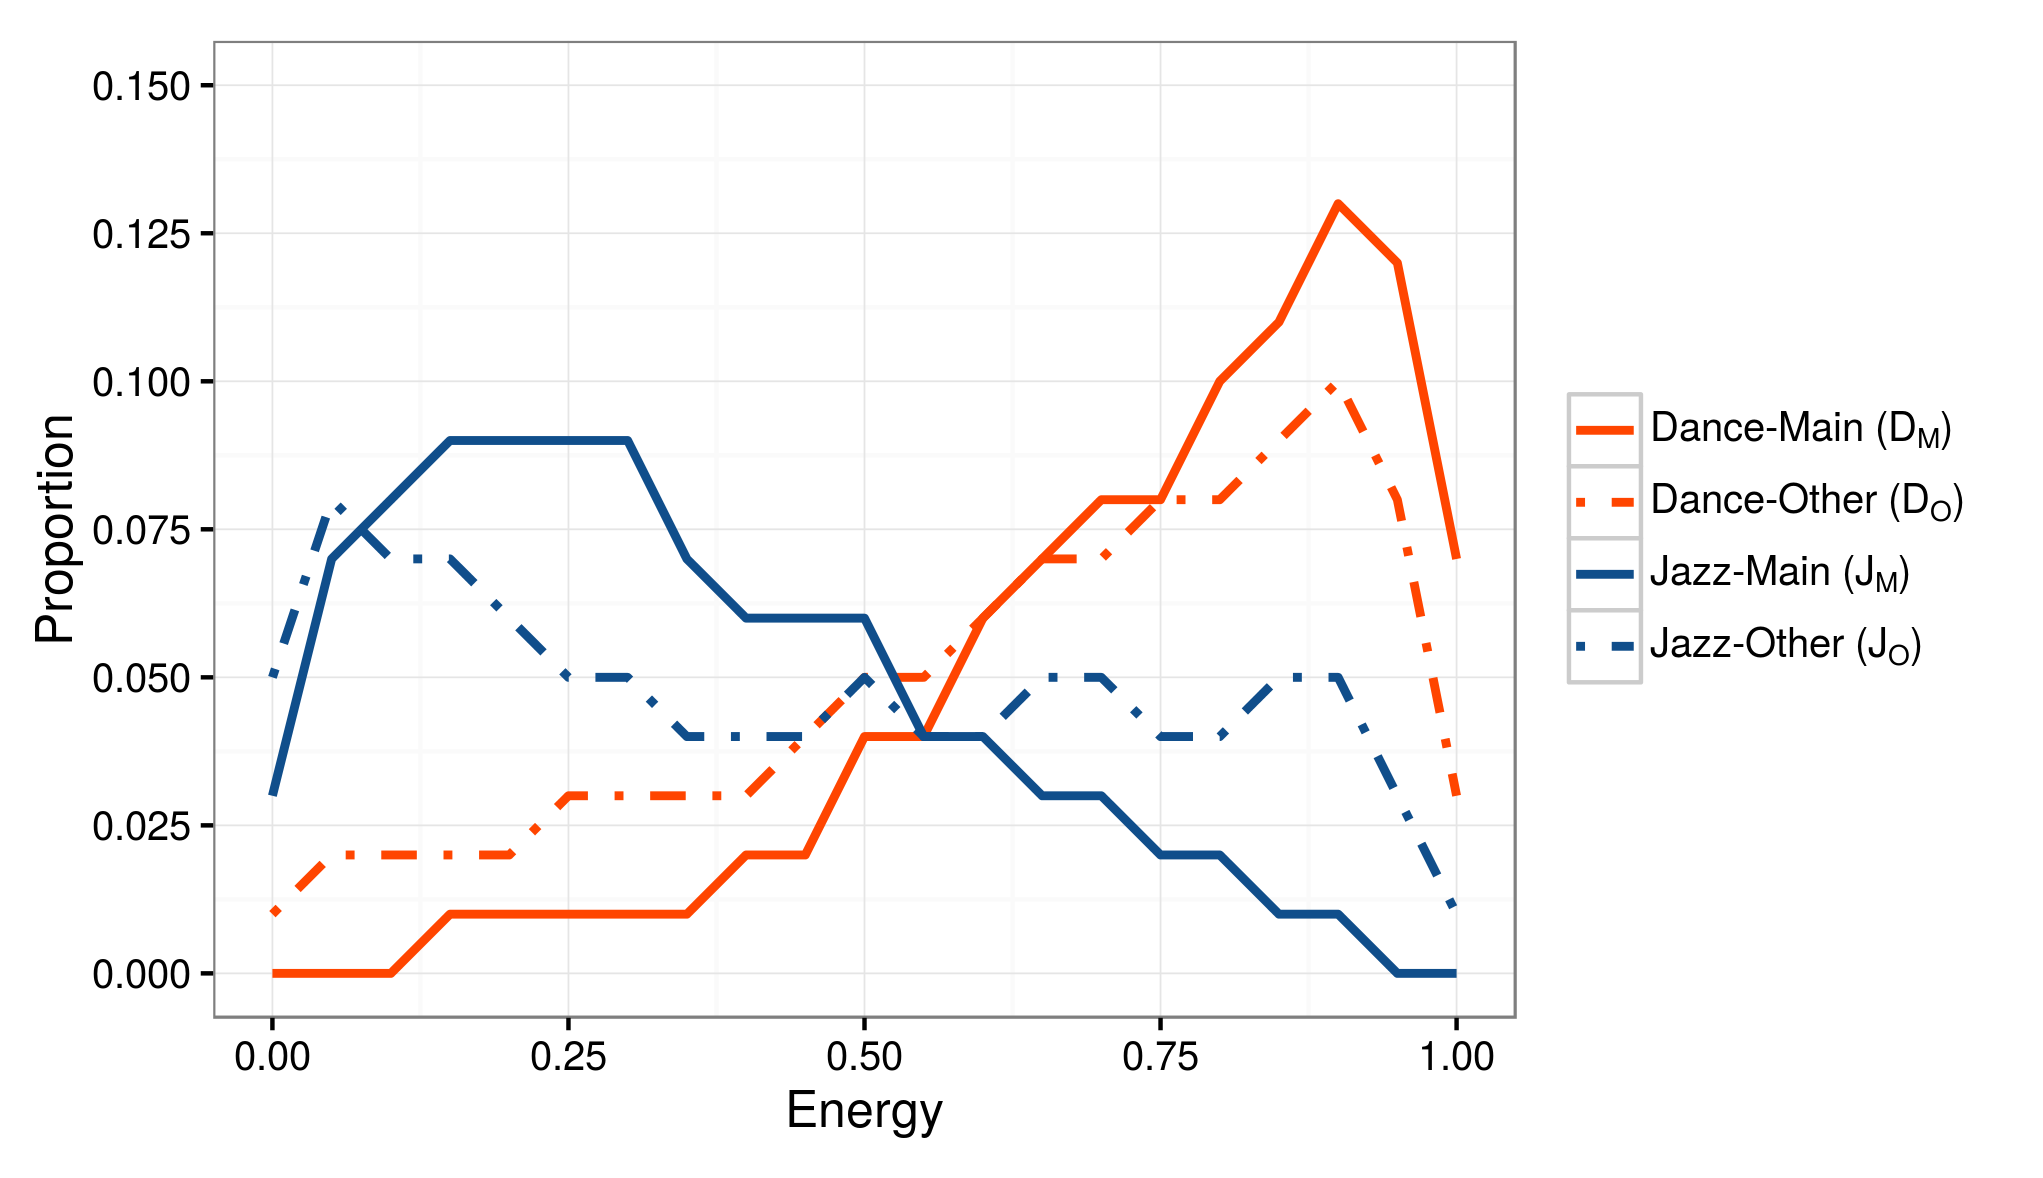
\includegraphics[width=\linewidth]{good_4lines}
\caption[Energy Distribution (Dance- and Jazz-heads)]{Energy distributions of tracks belonging to Dance-head and Jazz-head subgroups. The orange lines, $D_M$ and $D_O$, show the distributions of tracks downloaded by Dance-heads; the blue lines, $J_M$ and $J_O$, show the distributions of  tracks downloaded by Jazz-heads.}[]
\label{good_4lines}
\end{figure}

%FIGURE 2
\begin{figure}[h!]
\centering
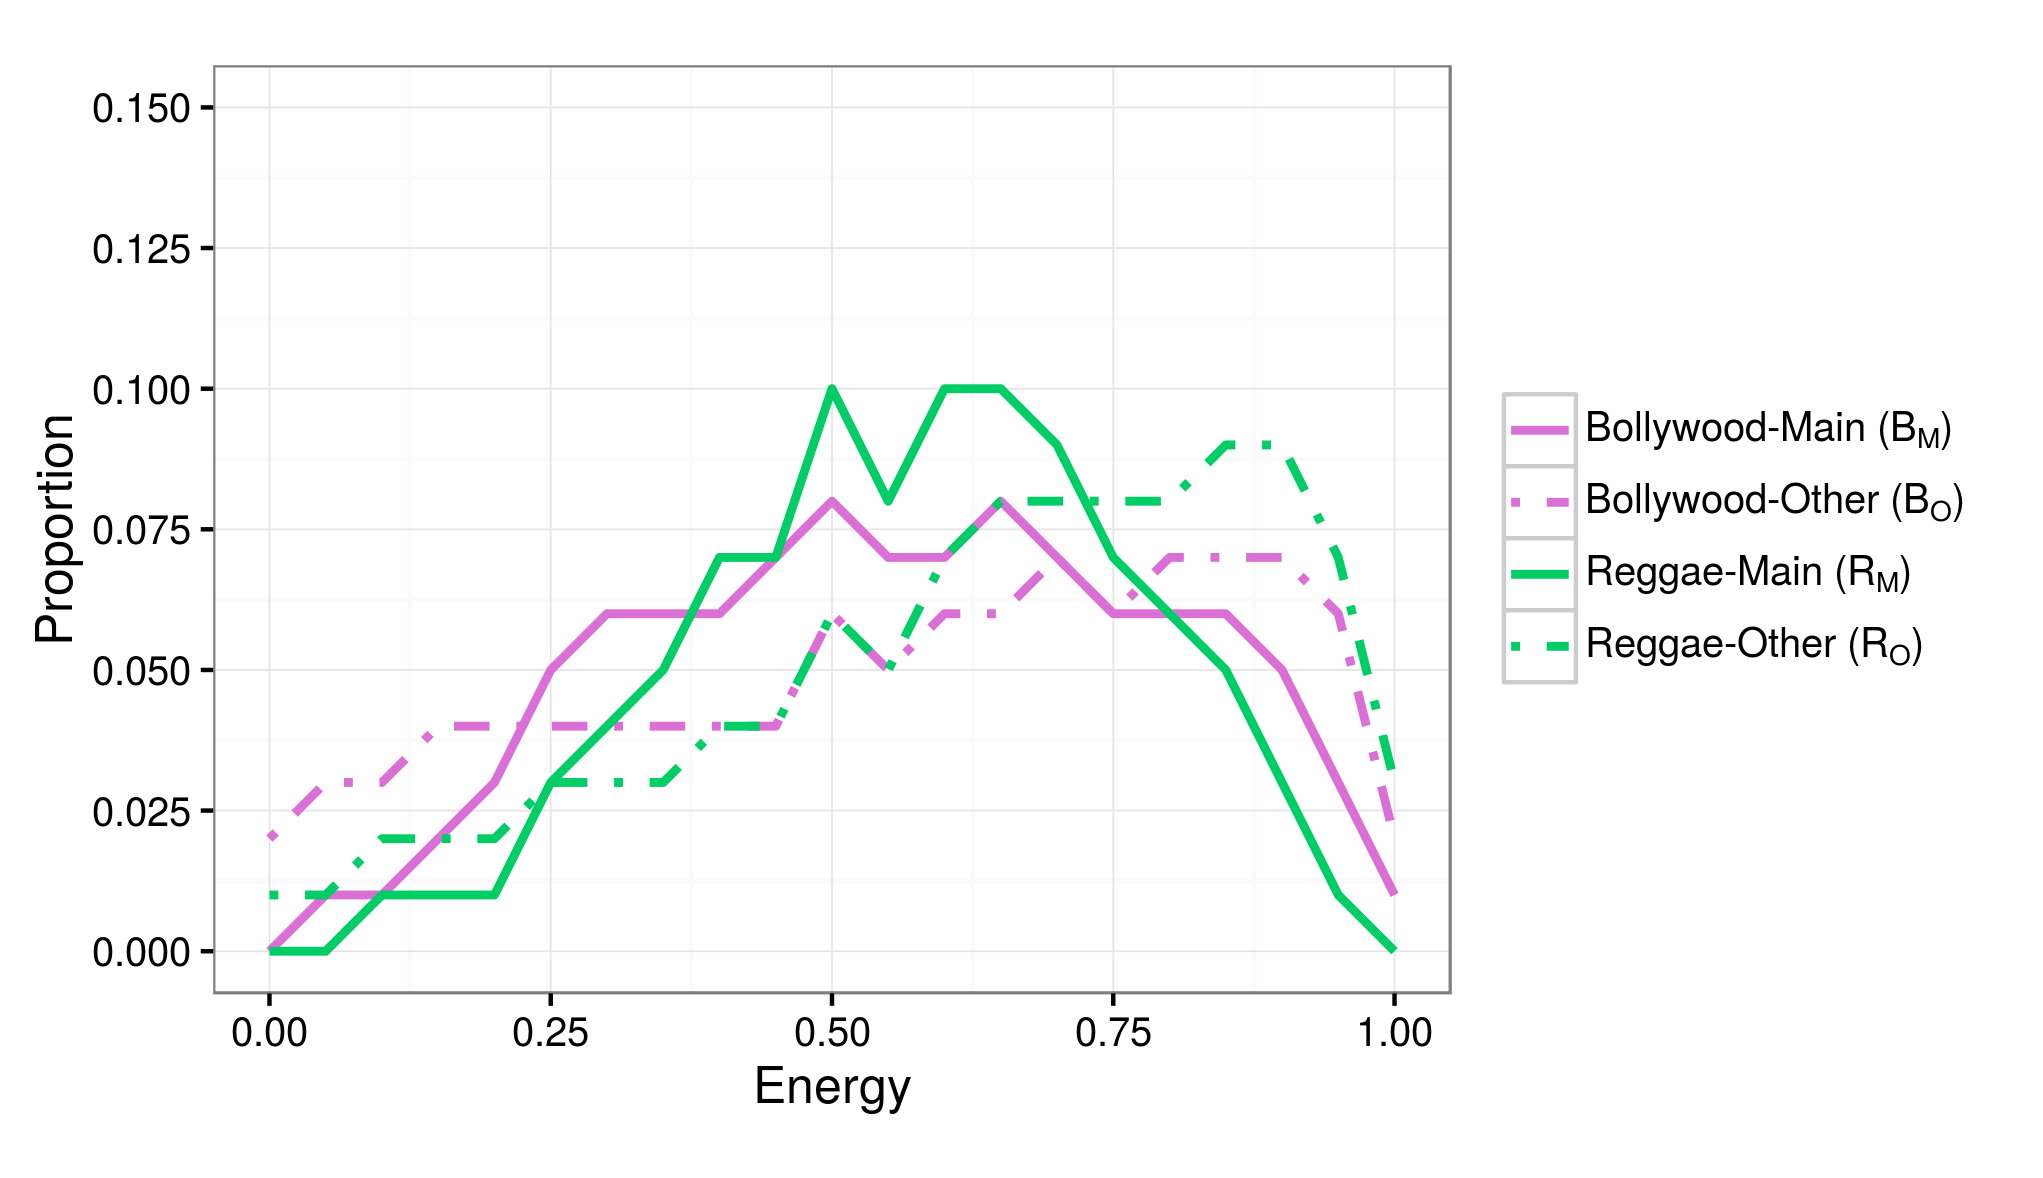
\includegraphics[width=\linewidth]{bad_4lines}
\caption[Energy Distribution (Bollywood- and Reggae-heads)]{Energy distributions of tracks belonging to Bollywood-head and Reggae-head subgroups. The purple lines, $B_M$ and $B_O$, show the distributions of tracks downloaded by Bollywood-heads; the green lines, $R_M$ and $R_O$, show the distributions of tracks downloaded by Reggae-heads.}
\label{bad_4lines}
\end{figure}

%FIGURE 3
\begin{figure}[h!]
\centering
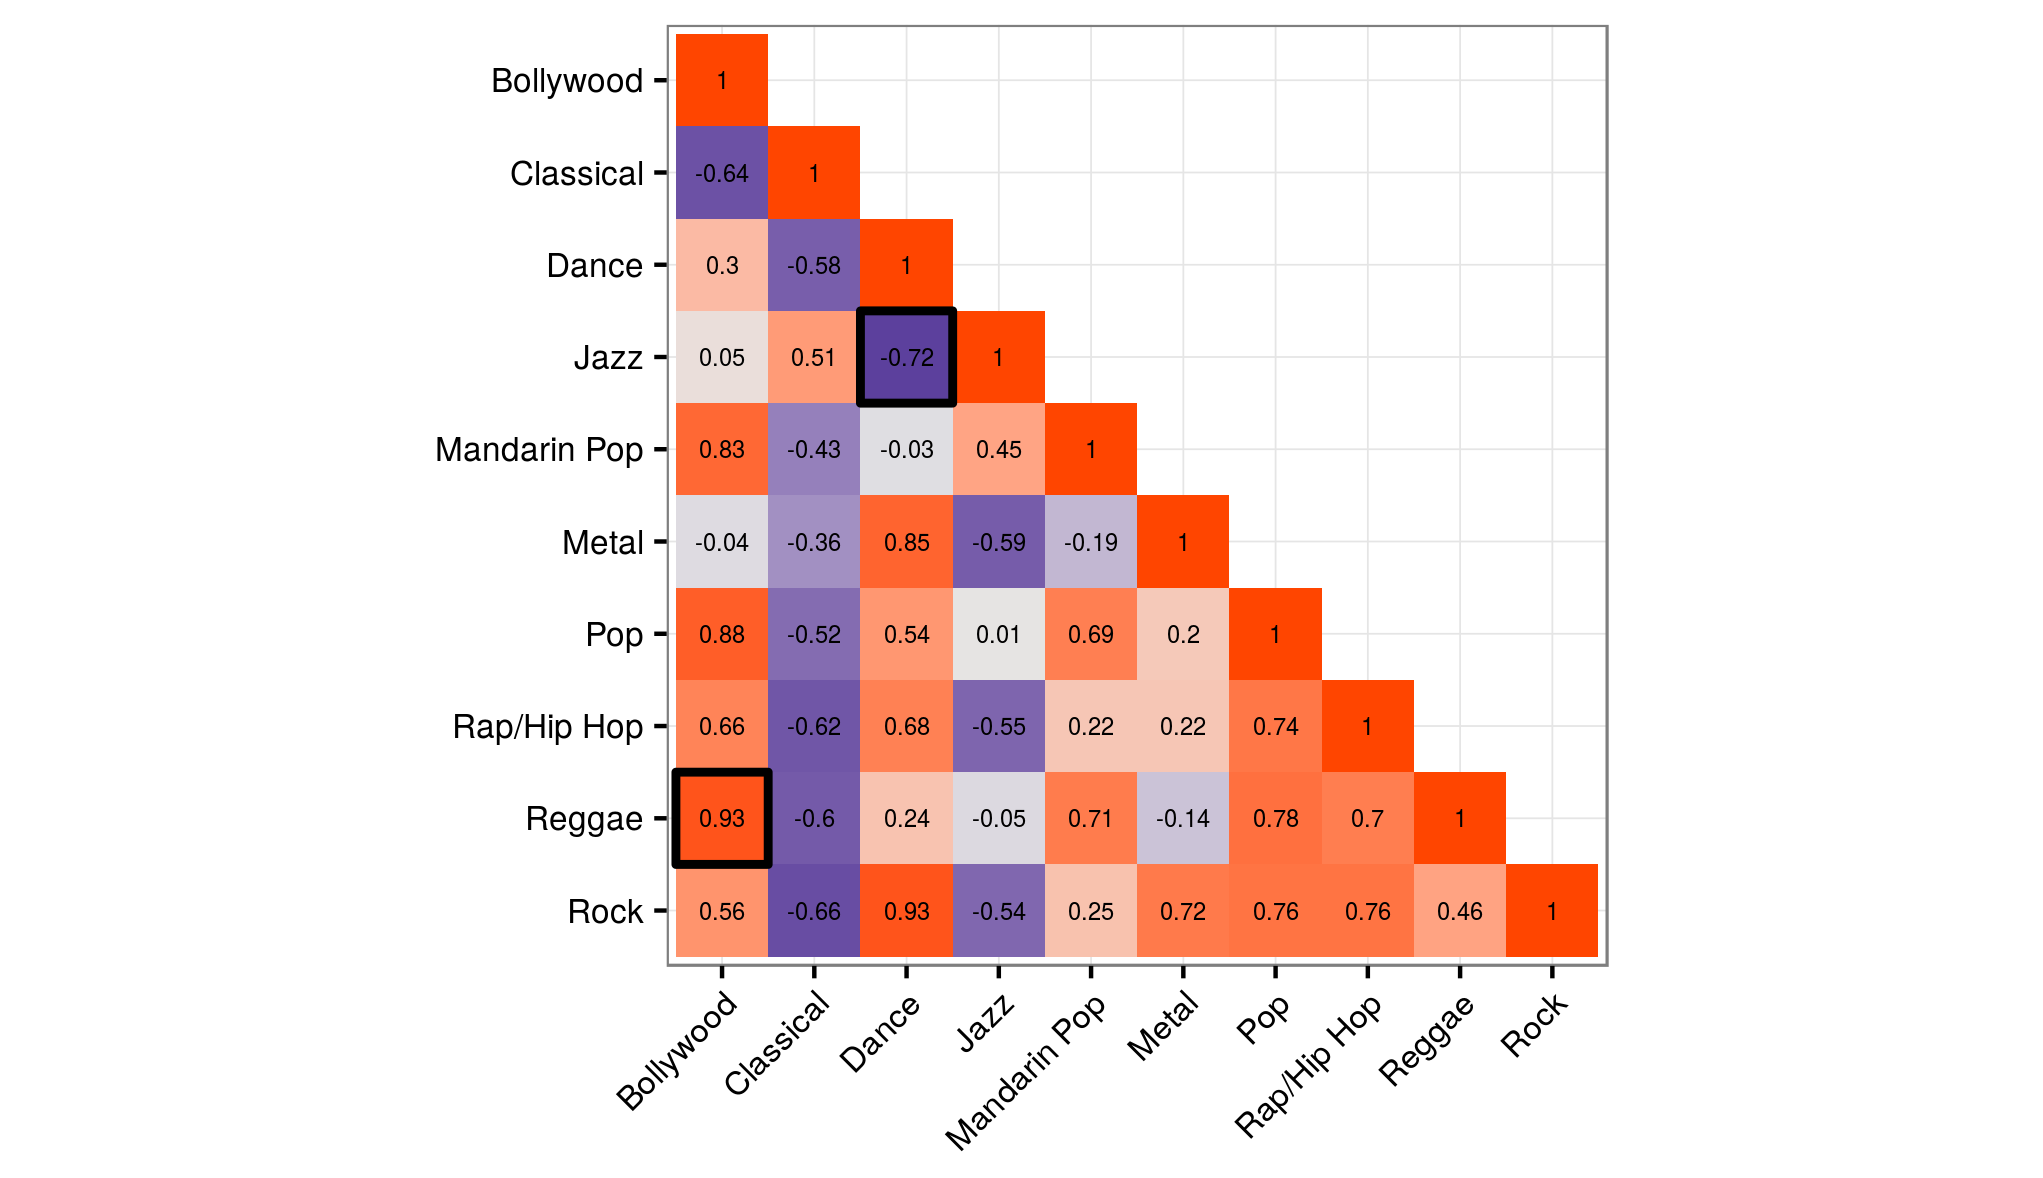
\includegraphics[width=\linewidth]{Energy_corrMat}
\caption[Energy Correlation Matrix]{Correlation Matrix for Energy. The two highlighted cells relate to the solid lines in Figures \ref{good_4lines} and \ref{bad_4lines}, Dance and Jazz, and Bollywood and Reggae respectively.}
\label{energy_corrMat}
\end{figure}

\begin{table}[ht!]
\centering
\begin{tabular}{|c|c|c|}
\hline
\textbf{X-Head Subgroup} & \textbf{Users} & \textbf{Downloads}  \\
\hline
Pop & 3,215,135 & 74,421,204 (23.14)\\
Bollywood & 2,134,919 & 30,340,368 (14.21) \\
Mandarin Pop & 1,944,975 & 15,165,454 (7.80) \\
Rock & 349,205 & 23,489,799 (67.27)  \\
Dance & 163,388 & 1,676,634 (10.26)  \\
Rap/Hip Hop & 156,384 & 2,122,862 (13.57)\\
Metal & 94,015 & 4,513,560 (48.01)  \\
Classical & 45,903 & 2,260,496 (49.25) \\
Jazz & 22,644 & 1,131,941 (50.00) \\
Reggae & 13,530 & 240,615 (17.63) \\
\hline
\end{tabular}
\caption[X-Head Genre Distributions]{Descriptive statistics for X-head subgroups: number of users; number of downloads (average downloads per user). \label{tab:xheadTotals}}
\end{table}

As described above, the presence of negatively correlated distributions, shown in Figure \ref{energy_corrMat} with respect to Energy, enabled the influence of five features to be studied using the present methodology. In sum, Acousticness had 12 negatively correlated distributions, Danceability 10, Energy 19, Loudness 5, and Valence 9 (Appendix \ref{sec:appendix}). Figure \ref{tTest_Outline} shows boxplots of the five features within the analysis. The red boxes on the left of each graph represent the within X-head coefficients; blue boxes on the right are the between X-head coefficients. Paired-sample t-tests, conducted to compare the within X-head coefficients and between X-head coefficients, showed the following results (sig. 2-tailed): 

\begin{description}
\item[Acousticness.] Significant difference for within (M=0.749, SD=0.170) and between (M=0.250, SD=0.302) X-head coefficients; t(23)=11.887, p<0.0001.
\item[Danceabilty.] Significant difference for within (M=0.608, SD=0.225) and between (M=0.313, SD=0.288) X-head coefficients; t(19)=8.046, p<0.0001.
\item[Energy.] Significant difference for within (M=0.557, SD=0.233) and between (M=-0.174, SD=0.414) X-head coefficients; t(37)=9.110, p<0.0001.
\item[Loudness.] Significant difference for within (M=0.636, SD=0.270) and between (M=0.315, SD=0.301) X-head coefficients; t(9)=10.656, p<0.0001.
\item[Valence.] Significant difference for within (M=0.653, SD=0.113) and between (M=0.223, SD=0.199) X-head coefficients; t(17)=11.887, p<0.0001.
\end{description}

%FIGURE 4
\begin{figure}[h!]
\centering
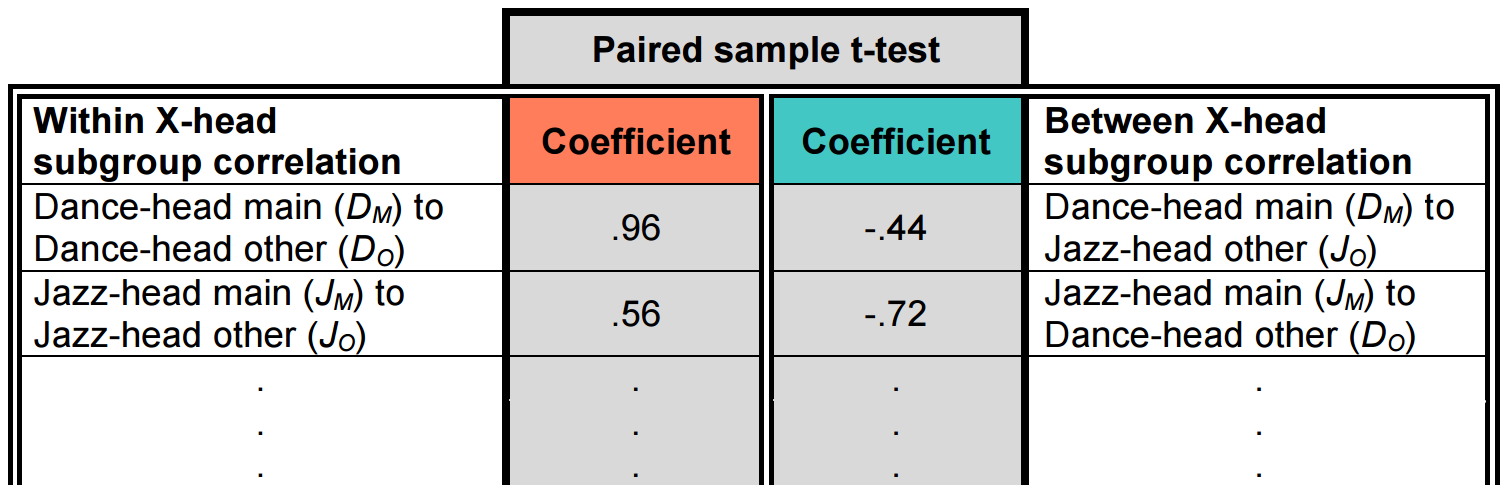
\includegraphics[width=\linewidth]{tTest_Outline.png}
\caption[Feature-Pair T-Test Analysis]{Example of paired sample t-tests with respect to Energy in which within-group coefficients were paired with between-group coefficients. Only the first two from 38 pairs are shown.}
\label{tTest_Outline}
\end{figure}

The statistics above confirm what is clearly evident in the boxplots in Figure \ref{Analysis_1_Boxplots}: there is a significant difference in the two sets of coefficients for each feature; in general, coefficients for the within condition are greater than the between condition. This is also true for feature Loudness, which had only five X-head pairs with negatively correlated distributions (producing ten pairs of coefficients). In other words, even with a relatively low \textit{n}, there is a significantly closer relationship between the features of an X-head’s main genre and their other music than with the features of a different X-head’s other music, i.e. a significant influence of the main genre on music of secondary importance within people’s downloads.

\begin{figure}[h!]
\centering
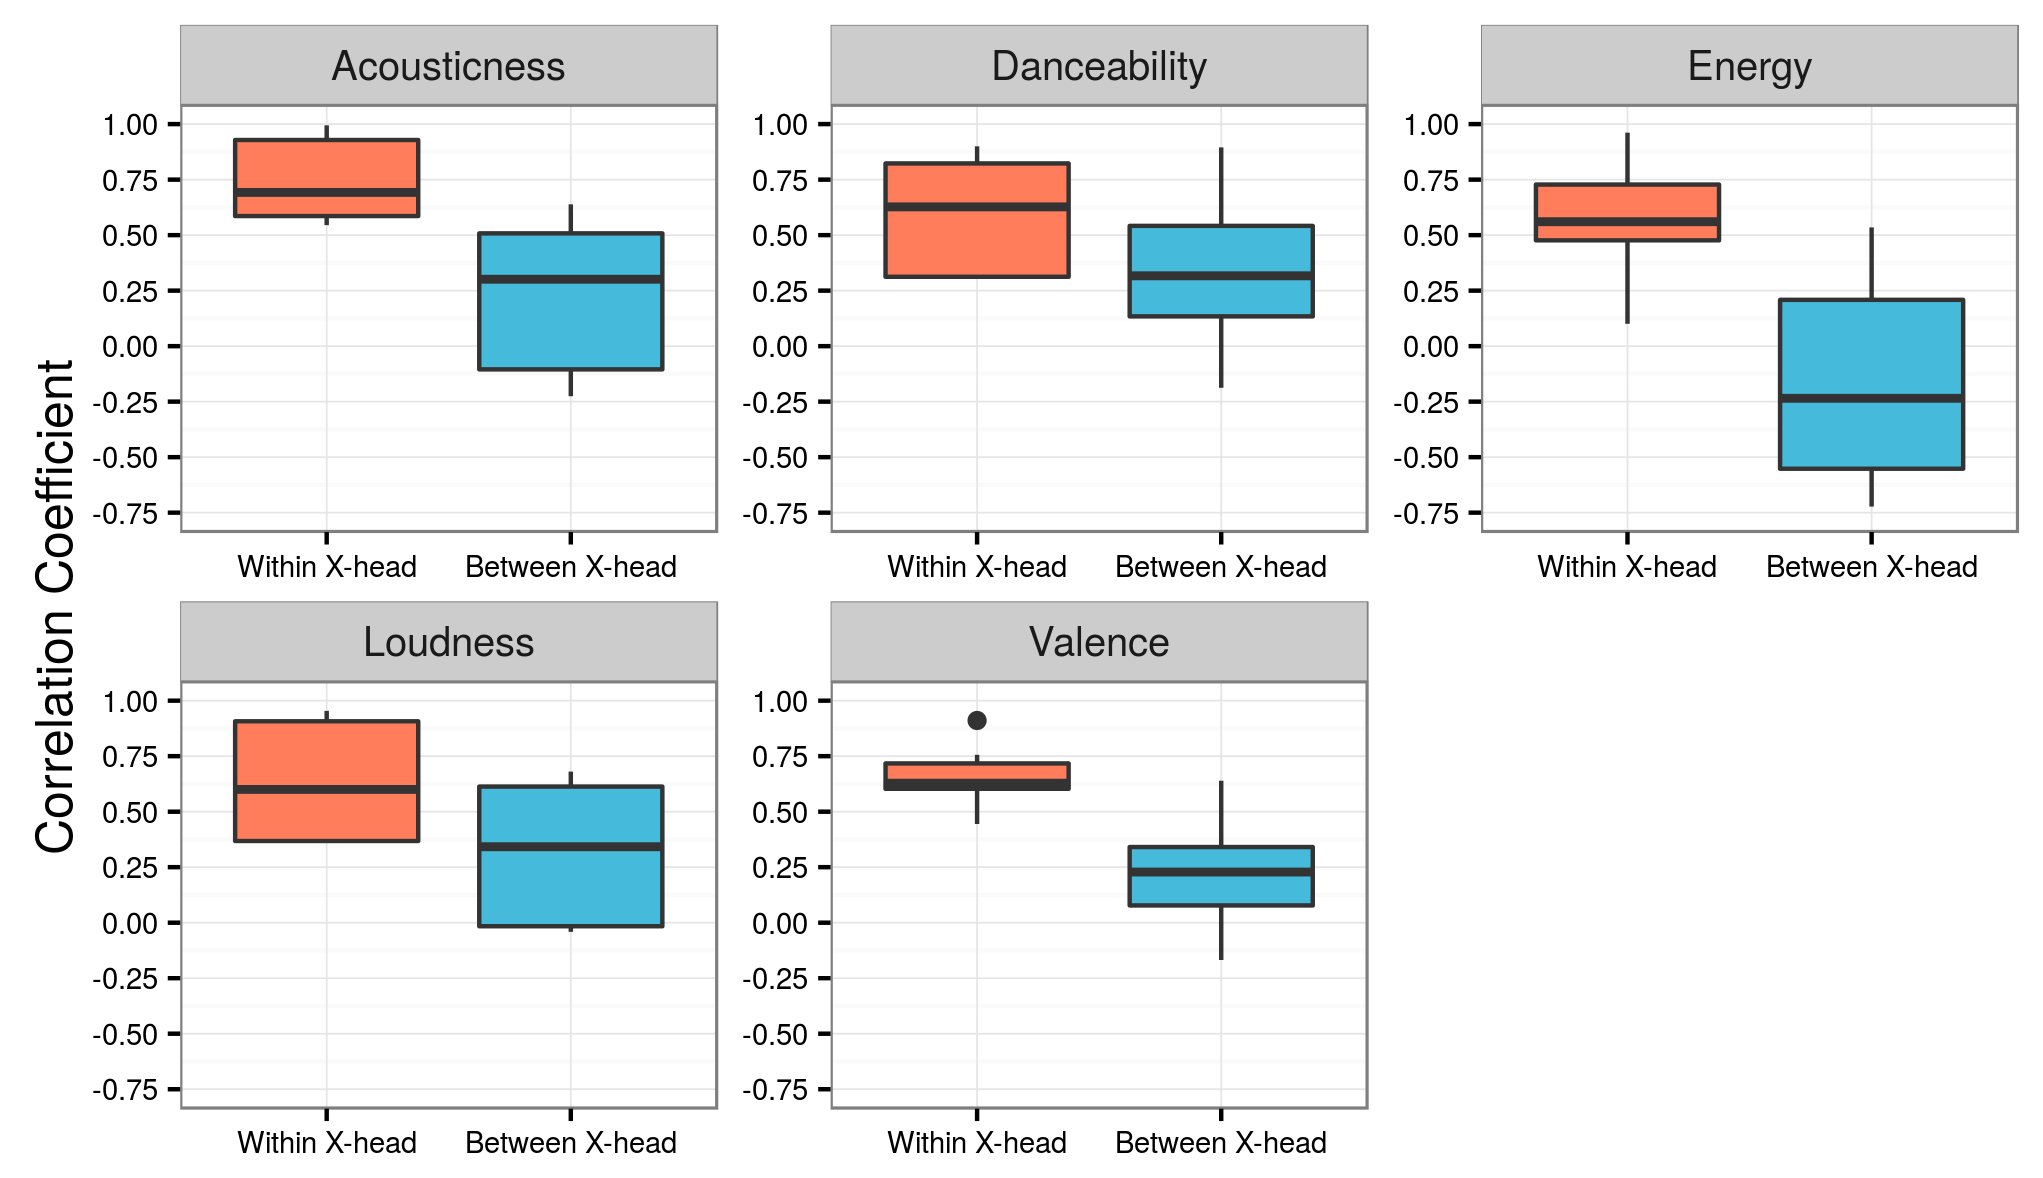
\includegraphics[width=\linewidth]{feature_BoxPlots.png}
\caption[Boxplot Feature Significance]{Boxplots of the five features within Analysis 1. Red boxes represent the within X-head coefficients; blue boxes represent the between X-head coefficients.}
\label{Analysis_1_Boxplots}
\end{figure}

\subsubsection{Analysis 2: Feature influence Matrices}\label{sec:leaky_anal_2}
Despite the results having a clear direction, the current method was not able to test the influence of five of the ten features within the analysis: Duration, Instrumentalness, Liveness, Speechiness, and Tempo. Although the observed pattern of influence may well extend to these features, this is by no means certain—for cognitive and neurological reasons, this phenomenon may be limited to particular acoustic features; for example, perhaps those that are more closely tied in some way to personality (e.g. \cite{mccown1997role}). Moreover, Analysis 1 was not able to address whether some X-head subgroups exhibited more influence, or if specific genres were more susceptible to being influenced by other genres more dominant within people’s download collections. For example, is it the case that Country is more prone to the influence of negatively valenced or sad music than, say, Metal? Similarly, might Jazz be more immune to the influence of up-tempo music than Bollywood, and what might be the interaction of X-head subgroup on these processes? The aim was not necessarily to explain such patterns, which may well involve a confluence of personality and sociocultural factors, but rather to observe the degree to which they existed within Nokia DB. To this end, we undertook a second analysis in which detailed information relating to each X-head subgroup and our selected ten genres was brought to light.

Each feature-influence matrix, referred to as C, was calculated from two submatrices, A and B. A, a 10 (X-heads) x 10 (genres) submatrix, contained the average feature values of all songs within a genre downloaded by an X-head subgroup (for example, the average value of Valence for all Reggae tracks downloaded by Classical-heads). B, a 10 (genres) x 1 (averages) submatrix, contained the average feature value of each genre downloaded by all users, excluding those made by the main X-head subgroup (for example, the value for Metal music determined by calculating the average Valence of Metal tracks downloaded by everyone except Metal-heads). C, the 10 (X-heads) x 10 (genres) feature-influence matrix, was calculated by subtracting the row values in A (subtrahends) from those in B (minuends), and converting the resulting differences into percentage changes from the averages in B. Formally, the above is given by: 

\begin{equation}
F = \{ \forall x_g \in F_{xg}, x_g = \{\frac{F_{xg} - P_g}{P_g} * 100 \} \} \\
\label{eqn:user}
\end{equation}
Where:
\begin{description}
\itemsep0em 
\item[$F$] = Feature-influence matrix (Matrix C)
\item[$x$] = X-head subgroup
\item[$F_{xg}$] = Average feature value for genre $(g)$ in X-head $(x)$ subgroup (Submatrix A)
\item[$P_g$] = Average feature value for genre  $(g)$ for entire population (Submatrix B)
\item[$x_g$] = Average feature value for genre $(g)$ listened to by X-head subgroup $(x)$
\end{description}

We illustrated this process with reference to Submatrices A and B, and Matrix C (the feature-influence matrix), and feature Valence. For clarity, the calculation is simplified to include only three X-head subgroups and genres: Dance, Metal, and Pop.
 
\paragraph{Submatrix A}
Table \ref{tab:matA} shows Matrix A: rows (\textit{i}) represent X-head subgroups; columns (\textit{j}) represent genres downloaded by each X-head subgroup. For example, average Classical, Dance, and Metal Valence values for Dance-heads $(i=2, j=(1,2,3))$ are $(2,1) = 0.28, (2,2) = 0.41$, and $(2,3) = 0.37$ respectively.

\begin{table*}[ht]
\centering
\begin{tabular}{|c|c|c|c|}
  \hline
\textbf{} & \textbf{Classical} & \textbf{Dance} & \textbf{Metal} \\
  \hline
\textbf{Classical-heads} & 0.27 & 0.43 & 0.38 \\
 \hline
\textbf{Dance-heads} & 0.28 & 0.41 & 0.37 \\
 \hline
\textbf{Metal-heads} & 0.28 & 0.44 & 0.35 \\
\hline
\end{tabular}
\caption[Submatrix A Example]{Example of Submatrix A showing the average Valence of three genres downloaded by three X-head subgroups. Rows represent X-heads; columns represent  genres. \label{tab:matA}}
\end{table*}

\paragraph{Submatrix B}
Table \ref{tab:matB} shows Submatrix B: the columns are genres; the row is the average Valence of each genre, excluding members of that particular X-head subgroup. For example, the average Valence for Metal music downloaded by non-Metal-heads $(1,3)$ = 0.39.

\begin{table*}[ht]
\centering
\begin{tabular}{|c|c|c|c|}
  \hline
\textbf{} & \textbf{Classical} & \textbf{Dance} & \textbf{Metal} \\
  \hline
\textbf{Population average} & 0.28 & 0.47 & 0.39\\
\hline
\end{tabular}
\caption[Submatrix B Example]{Example of Submatrix B for feature Valence with three genres. Rows represent genres; column represents the average feature value of a downloaded genre, excluding members of that particular X-head subgroup.\label{tab:matB}}
\end{table*}


\paragraph{Matrix C (Feature-Influence Matrix)}
Table \ref{tab:matC} shows Matrix C, generated by subtracting cell \textit{i,j} in matrix A from cell \textit{i,j} in Matrix B. We take the percentage change for that feature using the population average for a particular genre in Matrix B (similar results were obtained using population medians as opposed to averages). For example, to calculate cell (2,2) of Matrix C:
\begin{center}
$\displaystyle c_{i,j} = (\frac{A(i,j)-B(j)}{B(j)} ) * 100$\\
\vspace{0.5cm}
$\displaystyle c_{2,2} = (\frac{0.41 - .47}{.47} ) * 100 = \textbf{-12.8}$
\end{center}

This example indicates that Dance-heads downloaded Dance music that was 12.8\% more negatively valenced than the rest of the population downloading Dance.

\begin{table*}[ht]
\centering
\begin{tabular}{|c|c|c|c|}
  \hline
\textbf{} & \textbf{Classical} & \textbf{Dance} & \textbf{Metal} \\
  \hline
\textbf{Classical-heads} & -3.57\% & -8.51\% & -2.56\% \\
 \hline
\textbf{Dance-heads} & 0.0\% & \textbf{-12.8\%} & -5.12\% \\
 \hline
\textbf{Metal-heads} & 0.0\% & -6.1\% & -10.26\% \\
\hline
\end{tabular}
\caption[Matrix C Example]{Example of Matrix C, the Feature-Influence Matrix, showing the percentage Valence change of three genres downloaded by three X-head subgroups. \label{tab:matC}}
\end{table*}

Figure \ref{LF_Matrix_Val} shows the feature-influence matrix for Acousticness. Cell values indicate the percentage change in Acousticness of genres (columns) downloaded by X-head subgroups (rows), compared to the average Valence of genres downloaded by the overall population. The highlighted diagonal cells (running top-left to bottom right) show X-heads with respect to their main genres. The highlighted column on the right shows the median value of each row, excluding diagonally highlighted cells. 

%FIGURE 6
\begin{figure}[h!]
\centering
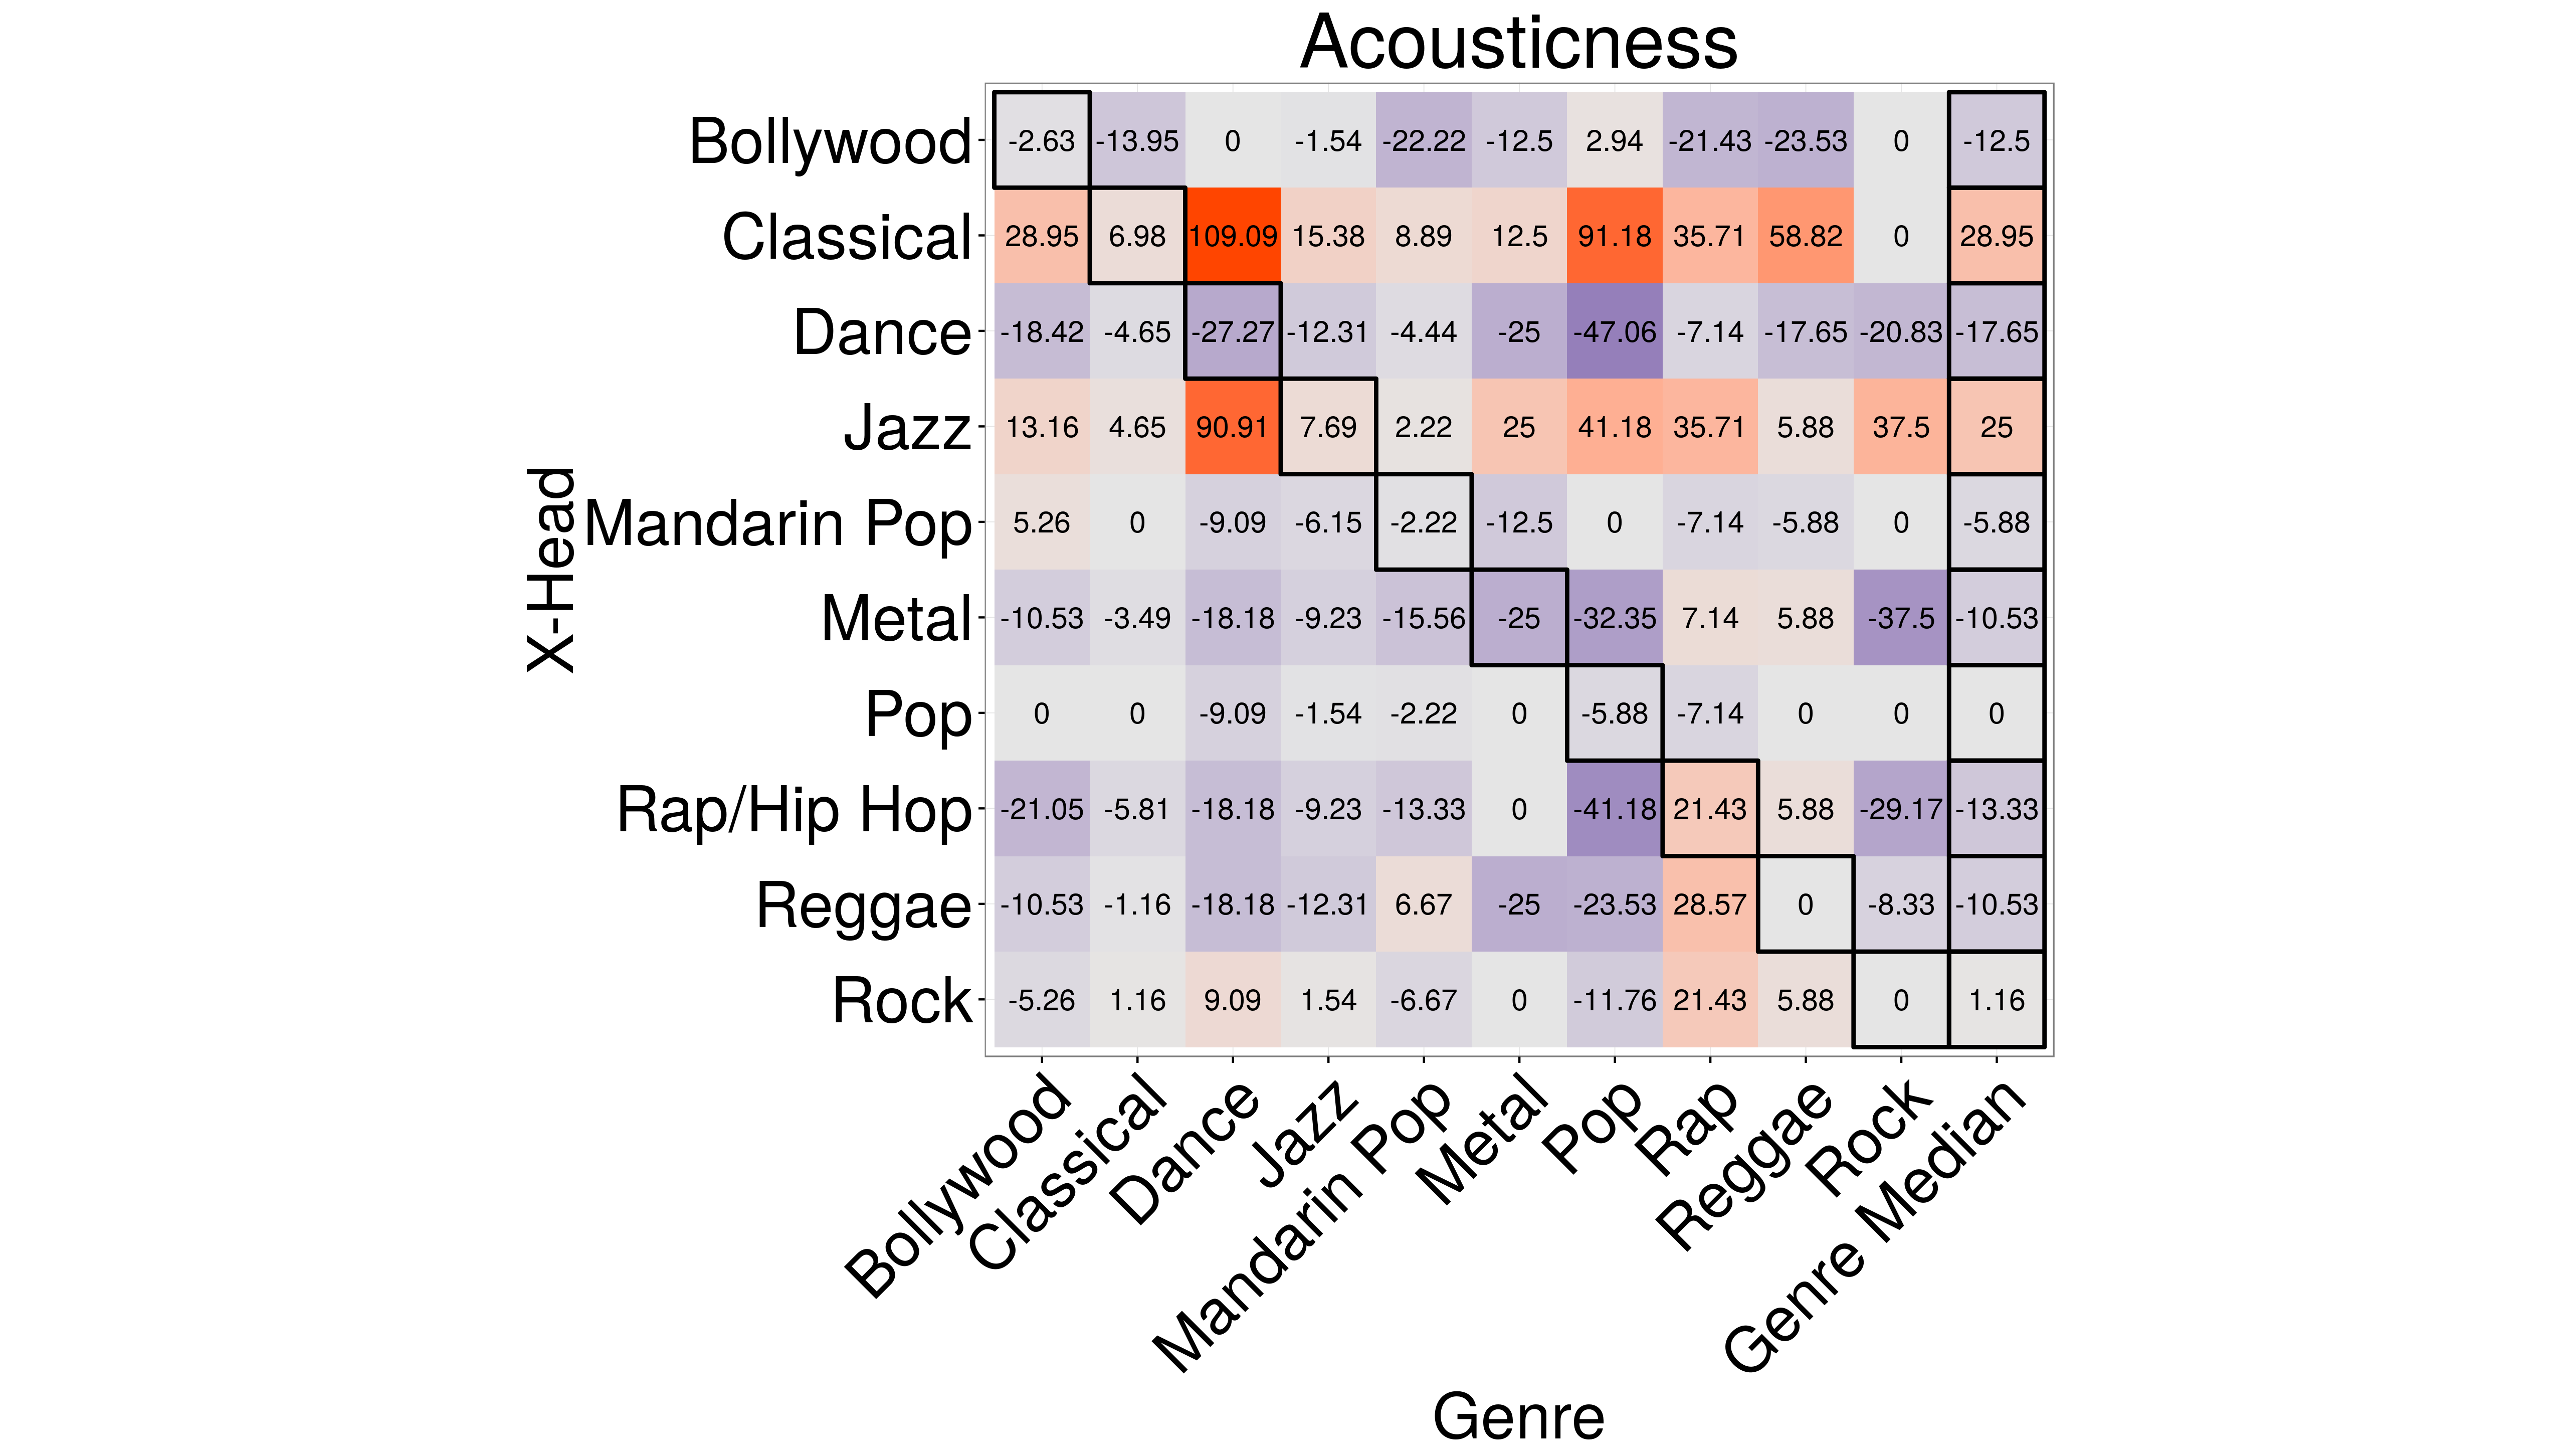
\includegraphics[width=\linewidth]{Acousticness}
\caption[Acousticness-influence matrix]{Feature-influence matrix for Acousticness. The highlighted diagonal cells (running top-left to bottom right) show X-heads with respect to their main genres. The highlighted column on the right shows the median value of each row, excluding diagonally highlighted cells.} 
\label{LF_Matrix_Val}
\end{figure}

%FIGURE 7
\begin{figure}[h!]
\centering
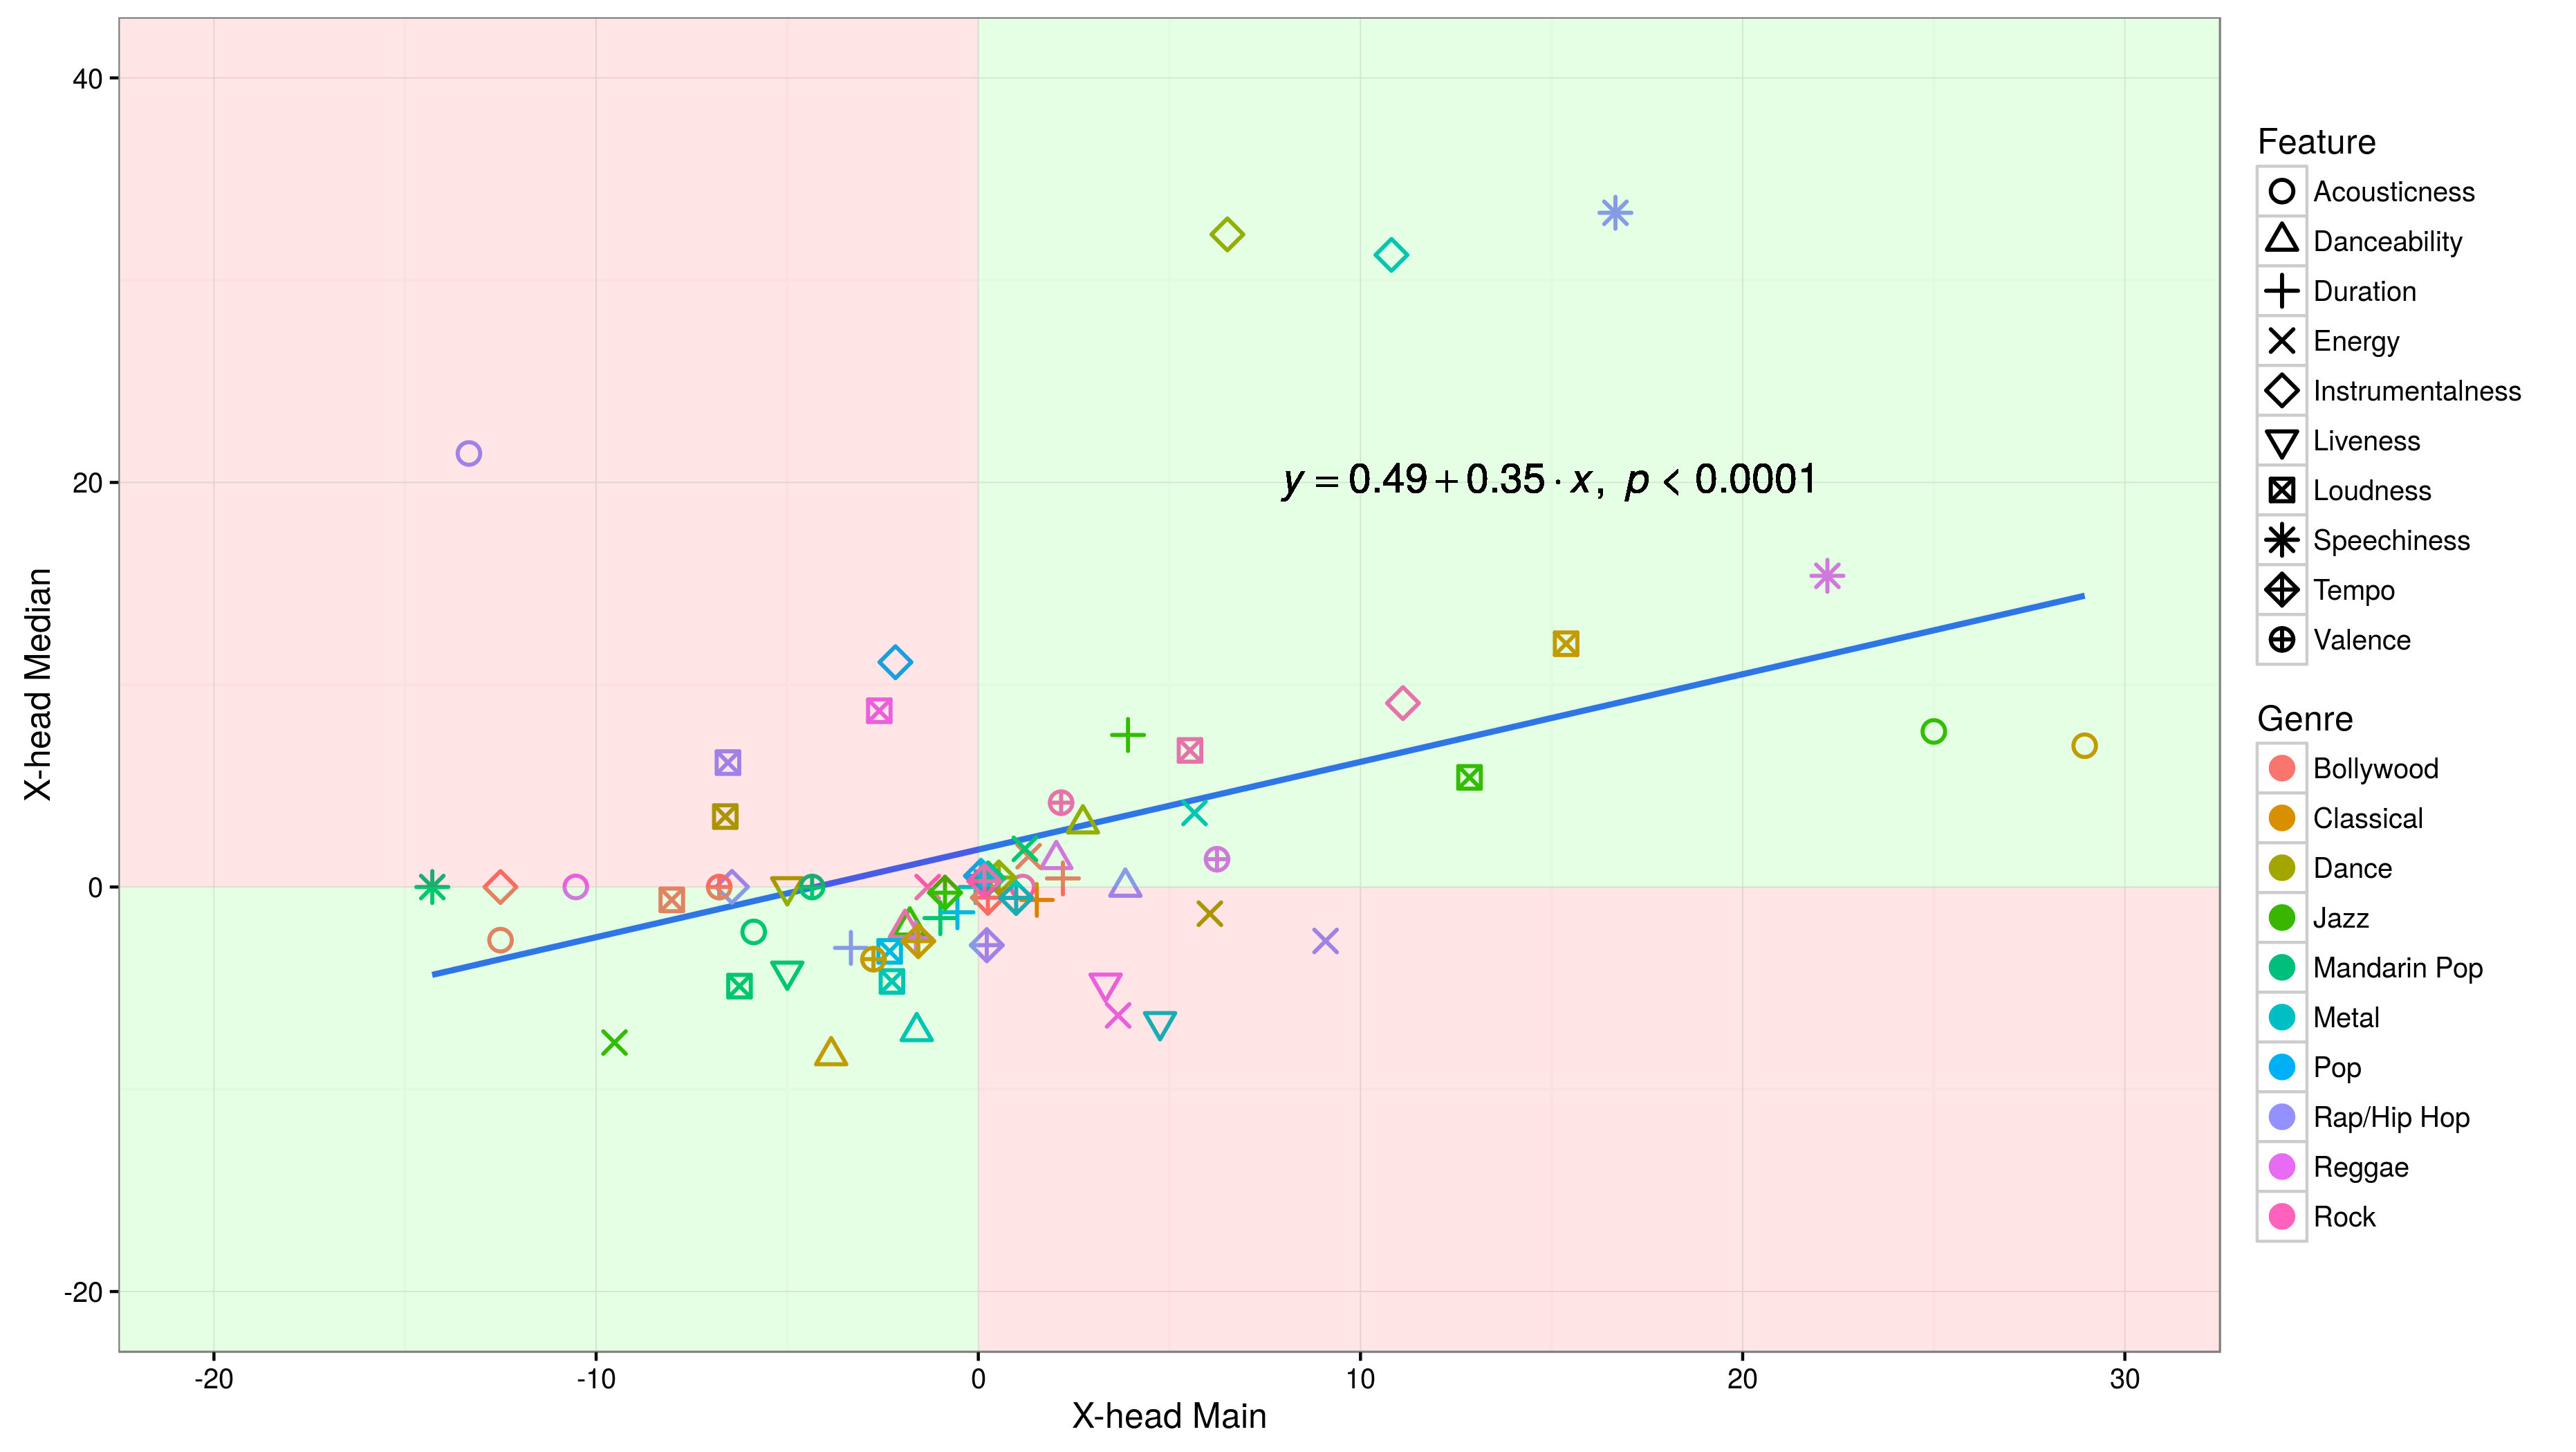
\includegraphics[width=\linewidth]{xScatter5}
\caption[Median-to-main Scatterplot]{Scatterplot showing the 100 diagonal-to-median cell pairings of the ten feature-influence matrices. Light-green quadrants indicate sign agreement between the row medians and X-heads with respect to their main genres, either positive or negative; pink quadrants indicate sign disagreement.}
\label{LF_Matrix_Scatter}
\end{figure}

Of the 100 possible diagonal-to-median cell pairings (10 features x 10 X-heads), the signs of 64 were in agreement; 36 were in disagreement (see Supplementary Material B). These pairings are shown in the scatterplot in Figure \ref{LF_Matrix_Scatter}. Light-green quadrants indicate sign agreement between the row medians and X-heads with respect to their main genres, either positive or negative; pink quadrants indicate sign disagreement. The adjusted $r^{2}$ value, 0.1039, gives rise to the following statistic: \textit{r}=0.34, \textit{n}=100, \textit{p}<0.0001. The finding in the feature-influence matrices that 64 diagonal-to-median cell pairings were in agreement, with 36 in disagreement, strongly suggests that there is a directional relationship, either positive or negative, between the features of X-heads’ main genres and those of their other genres. This is confirmed in the scatterplot in Figure \ref{LF_Matrix_Scatter}, and associated correlation statistic ($r=0.34$), in which there was a significant, positive relationship between the variables. 

The feature-influence matrices enabled two further, complementary questions to be explored: (1) which feature of X-heads’ main genres most strongly influenced their other genres, and (2) which X-head subgroup’s main genre most strongly influenced their other genres across all feature. For example, is the relationship between X-heads’ main and other genres stronger for Energy than Danceability? This question was assessed by correlating X-heads’ main genres with the nine other genres in each of their download collections. This produced one overall coefficient per feature-influence matrix; the resulting ten coefficients were then ranked in order. The second question asked which X-head subgroup across all features had the closest relationship between their main genre and other genres. For example, do the features of Mandarin Pop-heads’ main genre more strongly influence the corresponding features of their other genres than is the case for Reggae-heads? This question was investigated by correlating each X-head’s main genre with the nine other genres in each feature-influence matrix. This produced one overall coefficient per X-head subgroup, and, as before, the resulting ten coefficients were ranked in order. The results of these analyses are shown in Tables \ref{tab:feature} and \ref{tab:xhead}. Rows represent ranks, either of features or X-heads, columns include Pearson product-moment correlation statistics. 

\begin{table}
\centering
\setlength\tabcolsep{4pt}
\begin{minipage}[t]{0.48\textwidth}
\centering
\begin{tabular}{|c|c|}\hline
\textbf{Rank} & \textbf{Feature} $(n=90)$  \\
  \hline
\textbf{1} & Speechiness; $r=0.52^{***}$ \\
 \hline
\textbf{2} &  Danceability; $r=0.48^{***}$ \\
 \hline
\textbf{3} & Loudness; $r=0.45^{***}$ \\
\hline
\textbf{4} &  Energy; $r=0.44^{***}$  \\
\hline
\textbf{5} & Acousticness; $r=0.28^{**}$ \\
\hline
\textbf{6} & Tempo; $r=0.19^{\dotr}$ \\
\hline
\textbf{7} & Duration; $r=0.17$ \\
\hline
\textbf{8} & Valence; $r=0.14$ \\
\hline
\textbf{9} & Liveness; $r=0.06$ \\
\hline
\textbf{10} & Instrumentalness; $r=0.04$ \\
\hline
\end{tabular}
\caption[Feature Preference Influence]{Table showing the ranked order of features. The feature column shows which feature of X-heads' main genres is closest to their other genres ($^{\dotr} = p < 0.1$; * $= p < 0.05$; ** $= p < 0.01$; *** $= p < 0.001$).} 
\label{tab:feature} 
\end{minipage}%
\hfill
\begin{minipage}[t]{0.48\textwidth}
\centering
\begin{tabular}{|c|c|}\hline
\textbf{Rank} & \textbf{X-head} $(n=90)$  \\
  \hline
\textbf{1} & Metal; $r=0.56^{***}$ \\
 \hline
\textbf{2} & Jazz; $r=0.49^{***}$ \\
 \hline
\textbf{3} & Dance; $r=0.45^{***}$  \\
\hline
\textbf{4} & Classical; $r=0.41^{***}$ \\
\hline
\textbf{5} & Rap; $r=0.28^{**}$ \\
\hline
\textbf{6} & Rock; $r=0.26^{*}$ \\
\hline
\textbf{7} & Bollywood; $r=0.14$ \\
\hline
\textbf{8} & Reggae; $r=0.11$  \\
\hline
\textbf{9} & Mandarin Pop; $r=0.09$ \\
\hline
\textbf{10} & Pop; $r=0.08$ \\
\hline
\end{tabular}
 \caption[Genre Preference Influence]{Table showing the ranked order of X-heads. The X-head column shows the subgroup with the closest relationship between their main genre and other genres, across all features ($^{\dotr} = p < 0.1$; * $= p < 0.05$; ** $= p < 0.01$; *** $= p < 0.001$).} 
 \label{tab:xhead} 
\end{minipage}
\end{table} 

In Table \ref{tab:feature}, the top-ranked feature was Speechiness ($r=0.52$)—the presence or absence of spoken words in tracks belonging to main genres appears to have created a preference for similarly “speechy” tracks in X-heads’ other genres. Similarly, the Danceability, Loudness and Energy of users' predominant tracks appear to have heavily influenced tracks of secondary importance. At the other end of the spectrum, there was little-to-no relationship tracks between X-heads’ main and other genres in terms of Liveness (whether a track was recorded at a live event) and Instrumentalness (whether a track was created using only instrumental sounds). 

The top-ranked X-head subgroups were Metal ($r=0.56$) and Jazz ($r=0.49$). The dynamic nature of much Metal music seems to have created a musical “fingerprint” that strongly expressed itself in the other genres Metal-heads downloaded. Likewise, Jazz-heads seem compelled to seek out music containing Jazz-like qualities when exploring non-Jazz music. Conversely, Mandarin Pop and Pop’s musical features did not significantly influence the other music downloaded by these X-head subgroups, perhaps because the features of these genre are relatively indistinct ($r=0.09$ and $r=0.08$ respectively).

\subsubsection{Analysis 3: X-head Strength}\label{sec:leaky_anal_3}
While Analysis 2 provides a novel method to determine the relative influence of features and general susceptibility to features by X-head in aggregate, what specific features contribute to each subgroup and the strength of the feature's effect remains unclear. For example, although Table \ref{tab:xhead} suggests that Metal-heads are most influenced by acoustic features found in Metal music and that speechiness is the most influential feature across subgroups, the degree to which speechiness is influencing Metal-heads (as opposed to loudness or valence) cannot be determined using this analysis. Furthermore, X-head categorization is determined by the majority downloaded genre in a user's collection and neither Analysis 1 or 2 consider the intensity of preference. When listening to non-main genres, what features are most important for an Jazz-head? Are Metal-heads whose download history contains 100\% Metal tracks more likely to prefer these high-tempo features than a Metal-head whose history contains 51\%? Analysis 3 examines the relationship between an X-heads intensity of genre preference and acoustic features of their selected music.

As described in Section \ref{sec:nokia}, user data is anonymous; X-head categories (the majority downloaded genre in a user's collection) were developed in order to group users into meaningful categories for examining music preferences. The degree of this majority (e.g. 80\% of downloads for a user corresponding to their X-head category, as opposed to 60\%) may be a useful metric for determining ``X-head intensity'' in a way that builds upon the previous analyses. Based on the 62 genres available in the database (Appendix \ref{sec:appendix}) and the X-head calculation described in Section \ref{sec:xhead}, the X-head intensity metric can hypothetically range from 0.016 ($\frac{1}{62}$) - 1.00. Figure \ref{fig:xweightDists} visualizes X-head intensity distributions for the 20 largest X-head subgroups for users with at least 20 downloads. The distributions qualitatively vary in normality, skewness, and kurtosis. Communities with the most spread distributions statistics (i.e. the lowest average, mode, standard deviation, skew and kurtosis) are considered, in general, more genre inclusive (heterogenous) because the distribution of intensities are less focused on a specific area; whereas the communities with the highest values are considered more genre exclusive (homogenous). The most heterogeneous communities using these distribution metrics for all genres include: Bollywood- ($Kurtosis=-0.900$), Ghazal- ($Skew=0.694$), Bhojpuri- ($\mu=0.428$), Khaleeji- ($\sigma=0.0086$), and Region/Other-heads ($Mode=0.33$). The most homogenous communities were Italiana- ($Skew=8.566, Kurtosis=78.64$), Classic Arab/Tarab- ($\sigma=0.569$), and Iskelda-heads ($\mu=0.767$). 41 communities had modes at the maximum value of 1.00, suggesting that distributions are generally non-parametric and overall users tend to download only one genre. For an exhaustive list of values, refer to Table \ref{tab:xheadDist} in Appendix Section \ref{sec:appendix}.

\begin{figure}[h!]
\centering
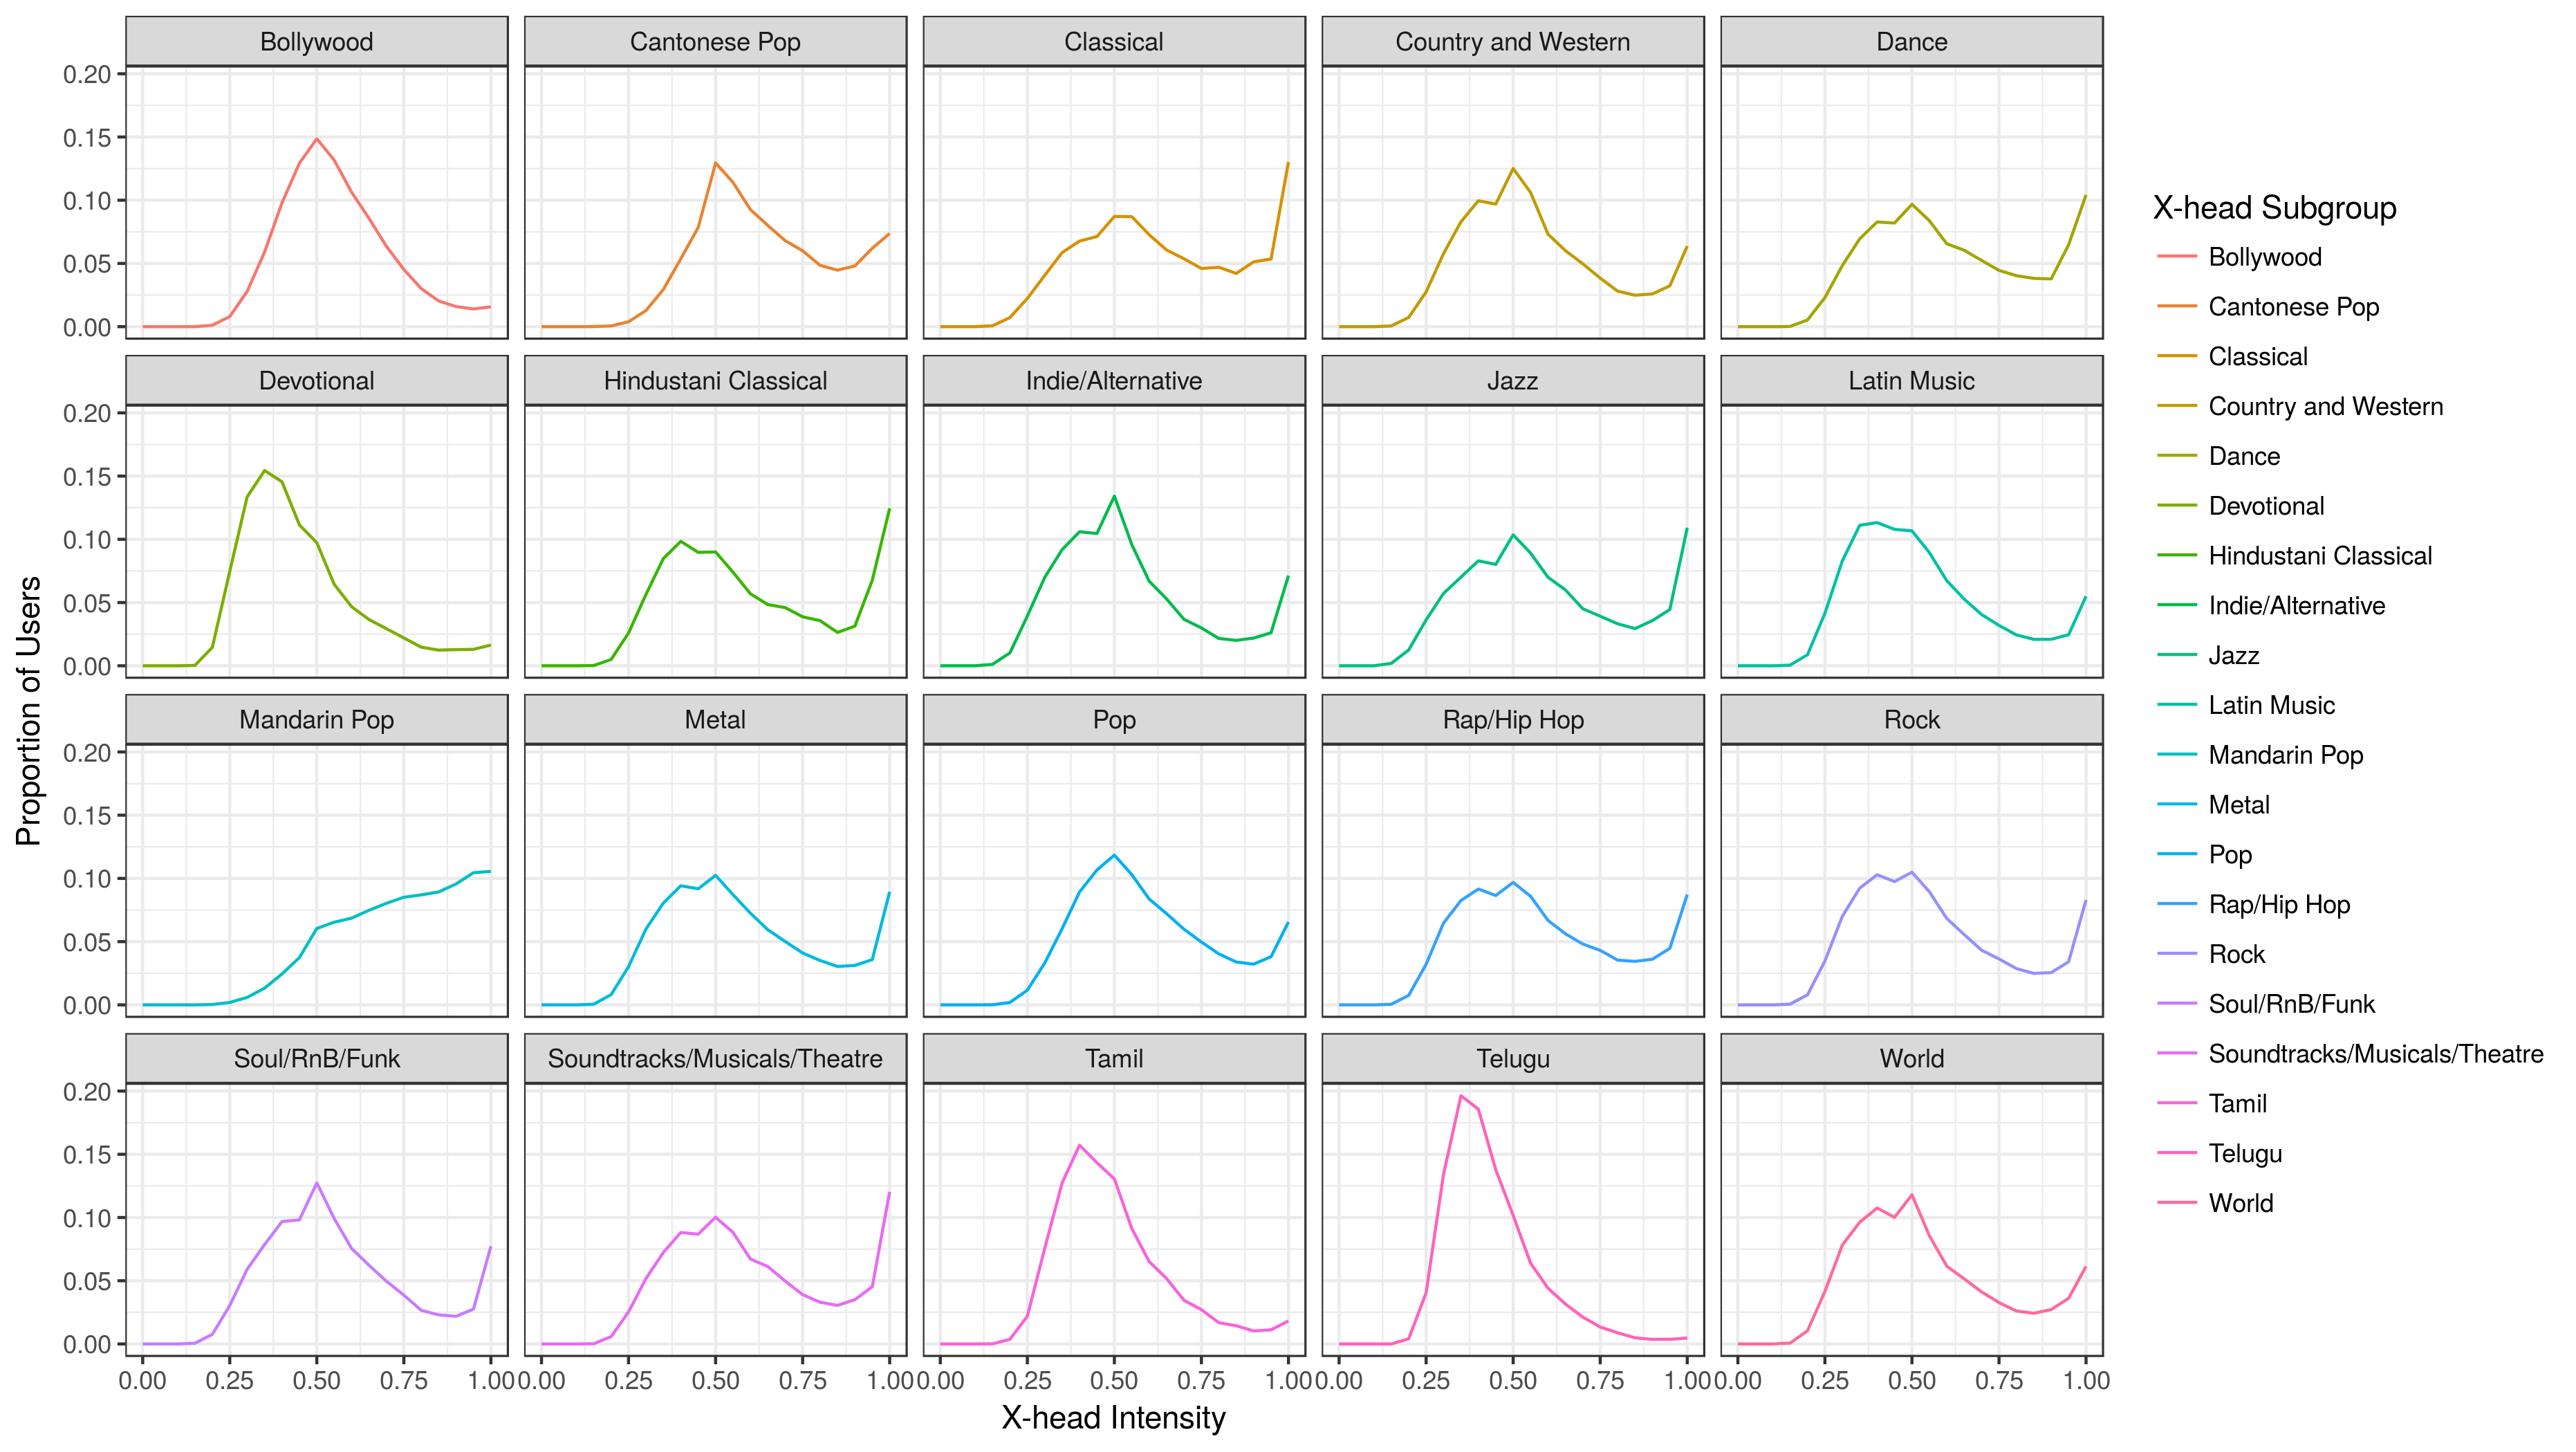
\includegraphics[width=\linewidth]{20_xheadDistributions}
\caption[X-head Distribution Sample]{X-head distributions for the top-20 subgroups for users with at least 20 downloads}
\label{fig:xweightDists}
\end{figure}

Because not all X-head subgroups exhibit normal distributions, non-parametric analyses were utilized. User's were aggregated into quartiles based on their intensities (labelled from one-to-four as: weak-heads, medium-weak heads, medium-strong-heads and strong heads) in order to balance unequal distributions across X-head subgroups. For example, users labelled as strong-heads will have an X-head intensity closer to 1.00, whereas weak-heads have intensities closer to the hypothetical minimum ($0.016$). Due to the population dynamics of this dataset, each subgroup contains a differing counts of total users, equally distributed across the four categories. Defining X-head intensity as ordinal quartile categories, rather than a continuous rational value is advantageous for two reasons: (1) analyses will not have an over-representation of any particular intensity (i.e. the analysis will not overfit to the mode X-head intensity of 1.00), and (2) it enables the use of two non-parametric tests which, and to what degree, acoustic features are influencing an X-head's preference when seeking out new music.

Jonchkeere-Terpstra trend tests (JT) \cite{cuzick1985wilcoxon} were used to evaluate whether there is a significant trend in ordered differences among categories. This test determines what features are producing a significant trend across X-head intensity. However, the JT does not provide a measure of effect size. To that end, a Kendall-Tau-$\beta$ test (KT) \cite{kendall1938new}, a non-parametric test similar to the JT is utilized in order to determine the effect size of specific features for X-head subgroups. Based on the success of analysis in Sections \ref{sec:leaky_anal_1} and \ref{sec:leaky_anal_2}, five additional X-head subgroups were included in this analysis: Blues-, Easy Listening/Oldies-, Indie/Alternative-, and World-heads. Because the JT and KT were developed for sample sizes which are orders of magnitude smaller than what is available in Nokia DB, bootstrapping with replacement was utilized. 100 random samples of X-head subgroups were generated. Each subgroup included 4000 users for each subgroup with equally distributed intensities (i.e. 1000 weak, medium-weak, medium-strong and strong users). Two subgroups (Blues and Country) were removed because they did not have at least 2000 users in each intensity category. The results of the 100 random samples of JT and KT tests for all ten features and 12 X-head subgroup were then averaged.

Figure \ref{fig:jtkt} and Table \ref{tab:jk} in Appendix \ref{sec:appendix} outline the averaged values from the 100 bootstrap samples for factors with at least marginally significant JT p-values only. 51 of 120 (14 X-head subgroups, each with 10 features) achieved marginal JT significance, 43 of 120 with significant JT test. The top 3 largest Kendall Tau-$\beta$ include: Speechiness by Easy Listening-heads ($\tau = -0.148$),  Speechiness by Rap-heads ($\tau = 0.124$), and Acousticness by Easy Listening-heads. Figure \ref{fig:jtkt} suggests that X-head's choose new music based on features that are hallmark in their preferred genre, and that they select music with features more similar to their preferred as their preference increases. The results provide additional support for trends found in Tables \ref{tab:feature} and \ref{tab:xhead} -- that some acoustic features and X-head subgroups are more sensitive or influenced by preference than others. Easy-listening/Oldies-, Classical-, Metal-, and Dance-heads are generally more influenced by their favourite genre than Pop-, Bollywood-, or Rock-heads; Speechiness, Loudness, Danceability are more often significant than Valence and Duration. The influence of some features and X-heads is different between Analysis 2 and 3. Features Instrumentalness and Valence, and the Reggae-head subgroup should not demonstrate an influence in preference according to Analysis 2, but qualitatively are some of the more represented tests in Analysis 3. Because Analysis 2 does not consider preference intensity, the differences in significance for some X-heads and acoustic features suggest that the degree to which a genre influences feature choice in secondary styles differs across subgroups.

\begin{figure}[h!]
\centering
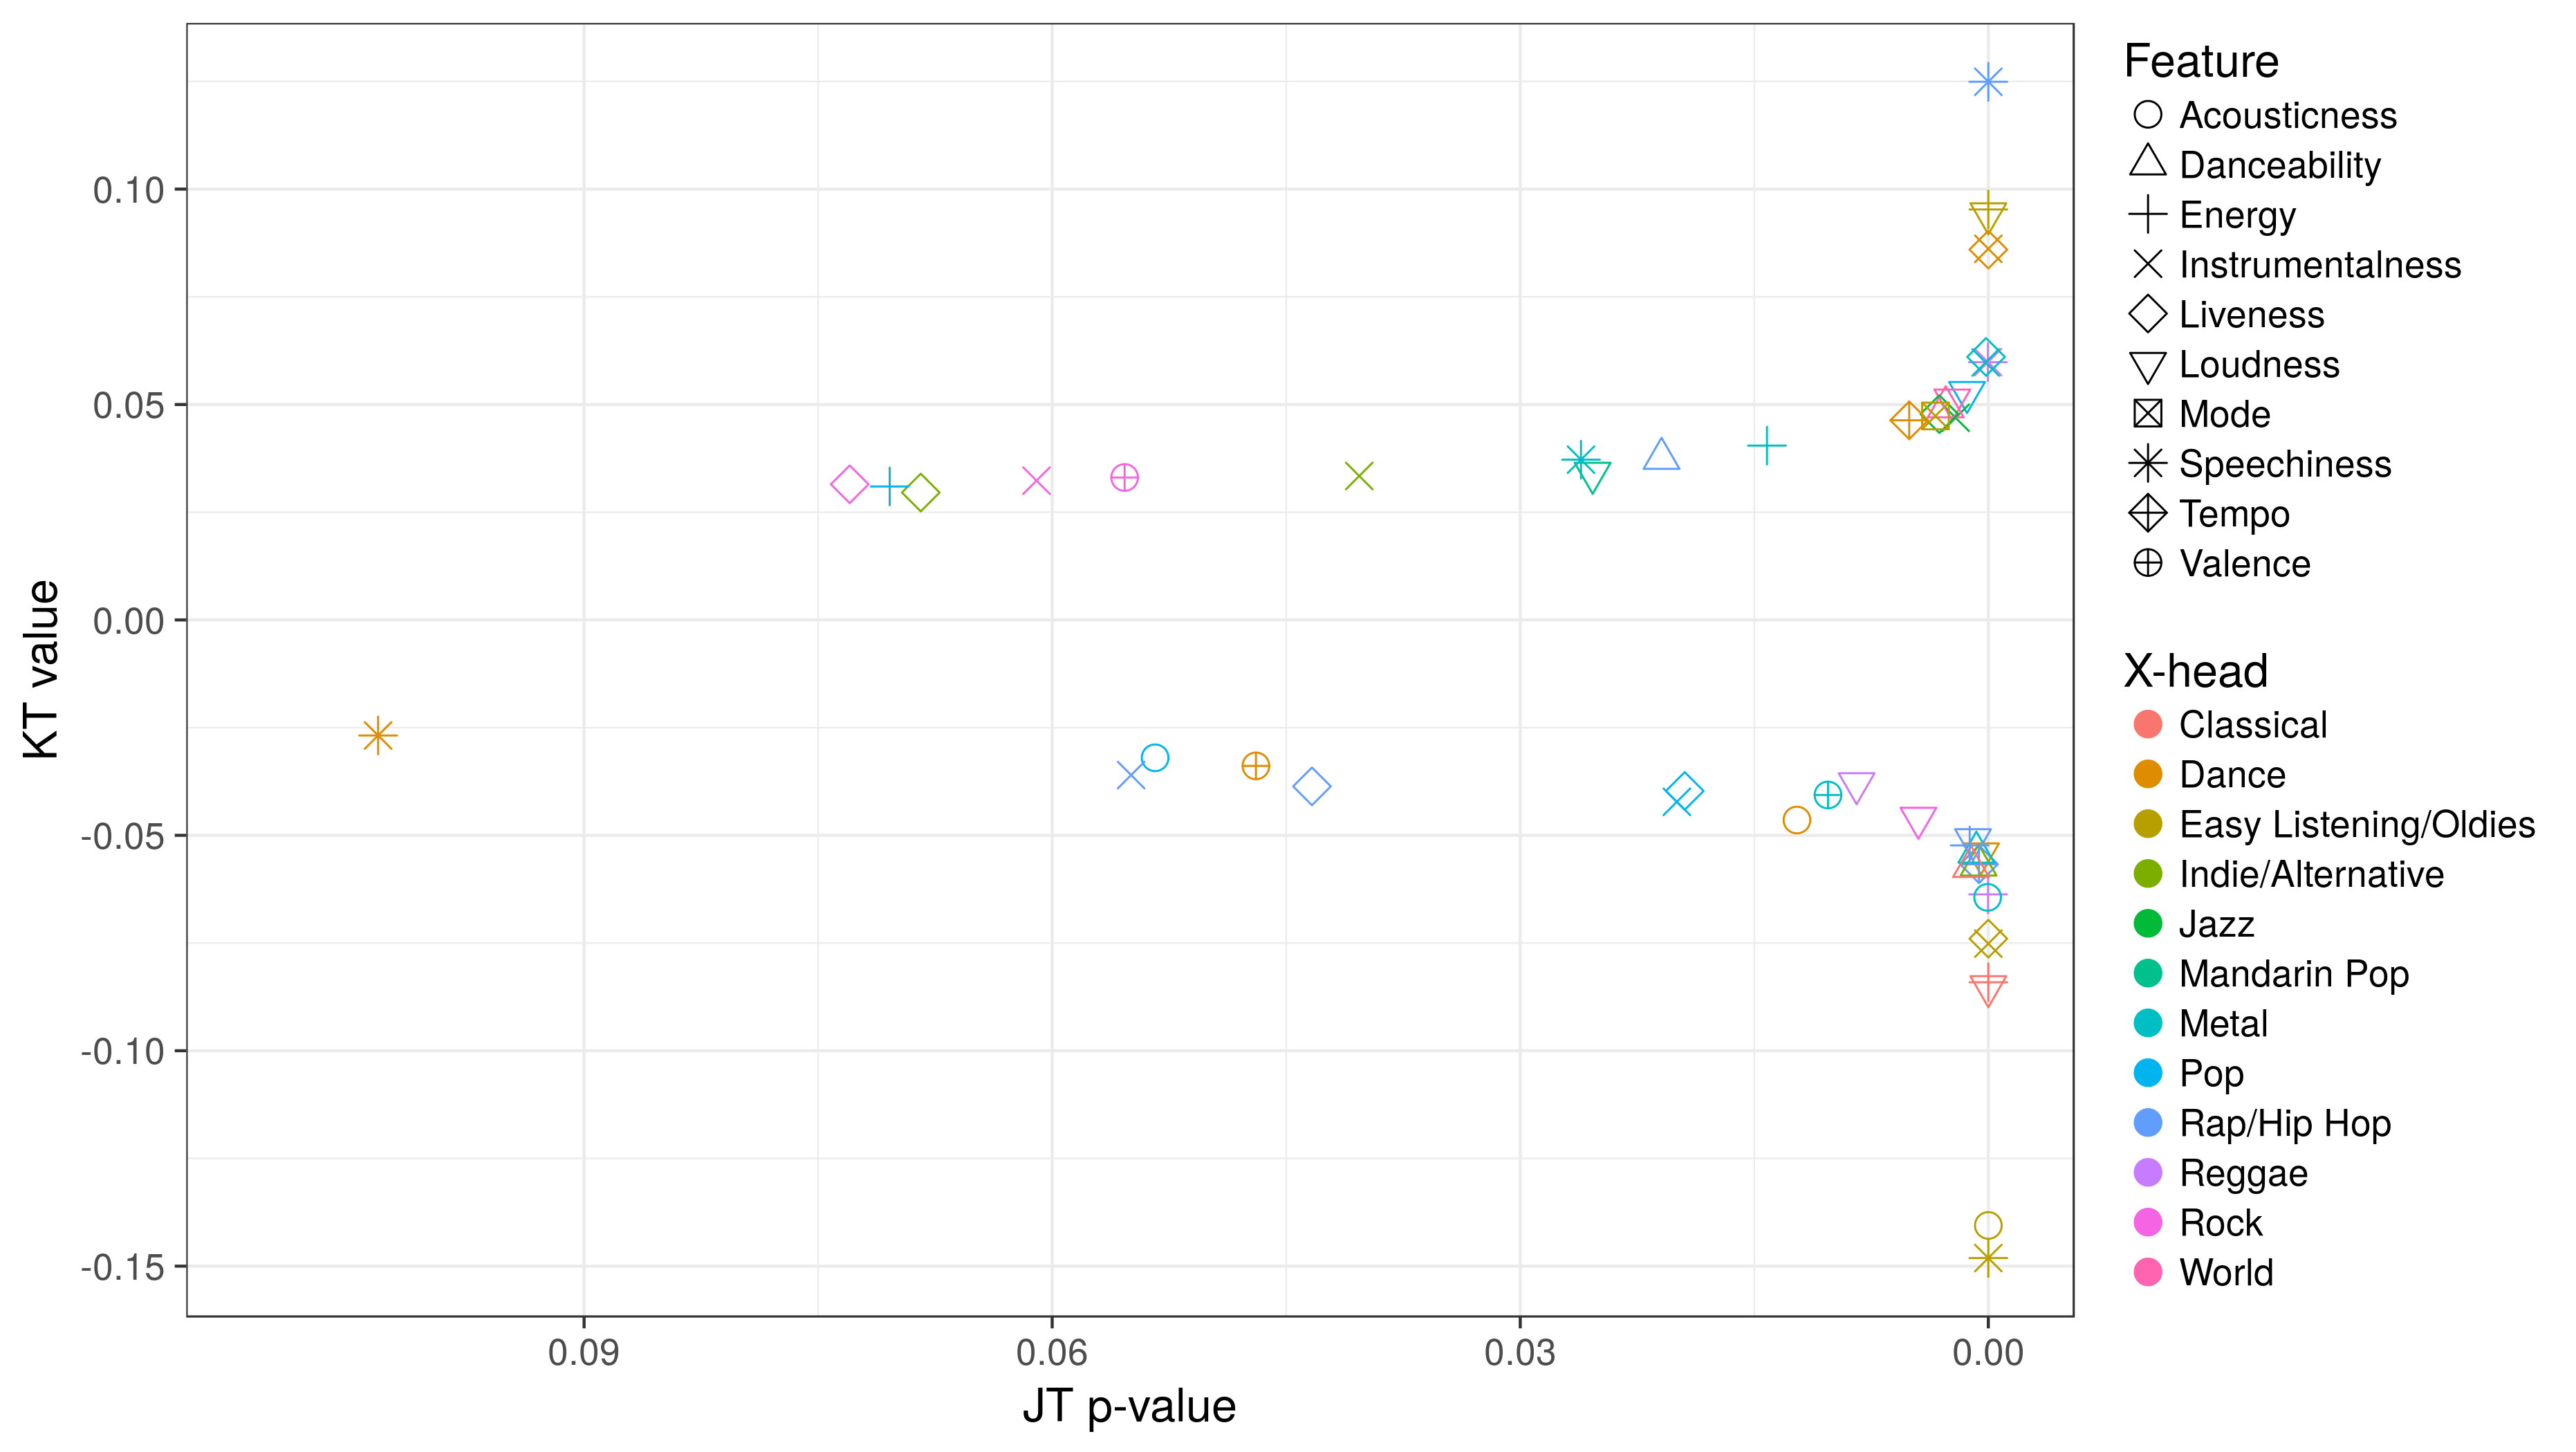
\includegraphics[width=\linewidth]{JTKTplot.png}
\caption[Jonckheere Terpstra-Kendall's Tau-$\beta$ Results]{Results of the non-parametric Jonckheere-Terpsra trend test (x-axis) and Kendall Tau-$\beta$ rank correlation (y-axis). Colours represent X-head tested subgroups and shapes represent tested features.}
\label{fig:jtkt}
\end{figure}


%%%%%%%%%%%%%%%%%%%%%%%%%%%%%%
\subsection{Ecleticism and Human Development}\label{sec:hdi}
While mood and personality pertain, to some degree, to an individual's artistic taste, shared demographic factors including culture, education, income, sex, and age also effect musical people's musical choices \cite{peterson1996changing,christenson1988genre,roberts1990music,leblanc1999effect,schafer2009functions,north2013musical}. Of these, age appears to be the strongest predictor of musical preference \cite{christenson1988genre}; older adolescents also prefer lighter qualities in music compared to younger adolescents \cite{roberts1990music}. General enjoyment of music from grade one to college drops for a time until rising around age of puberty, following a U-shaped curve across development \cite{leblanc1996music}. With respect to sex, a music-choice study suggests that males prefer music with themes of dominance and independence, whereas females preferred music with relationship and emotion themes \cite{christenson1988genre}. However, the extent to which this research is generalizable is open to debate: almost 30 years has elapsed since \cite{christenson1988genre}'s study, which was based on low-sample surveys with relatively little demographic variation. Furthermore, \cite{leblanc1999effect,north2013musical} found that demographic information did not conclusively determine music preferences; two- and three-way interactions were found between age, sex and country, and controlling for these factors significantly reduced the strength of the relationships. 

One of the most studied social psychological behaviours related to music preference is a concept known as "cultural omnivorism" (used interchangably with eclecticism), coined by Richard Peterson in the 1990s \cite{peterson1996changing,warde1999consumption,katz2002highbrow,katz2004cultural,chan2007socialmusic}. Peterson argues that for much of human history, music has been a means of stratifying groups across class and status, thus defining "highbrow" and "lowbrow" artistic styles. Traditionally, highbrow music was socially and economically expensive to participate in; instruments and concerts were costly (restricting access to low-class individuals), and learning music theory required education and time investments (restricting access to low-status and low-class individuals). However, as access to music began to become easier through technological advances (e.g. sheet music through printing press, radio, recorded sound, personal recording studios, and the internet), lowbrow consumers were able access and appreciate highbrow art, thereby negating the ability to stratify across class boundaries using music. \cite{peterson1996changing} argues that in order for highbrow to maintain stratification highbrow consumers transitioned from an elitist to eclectic to maintain class and status boundaries \cite{chan2005social}. Cross-cultural research generally supports the notion that diverse tastes are influenced by economic and education across many other types of consumption including: visual arts \cite{chan2005social}, television \cite{lizardo2009highbrow}, theatre \cite{chan2007socialvisual}, and restaurants \cite{warde1999consumption}. 

Other related user behaviours, such as voraciousness \cite{sullivan2007omnivore}, support the omnivore hypothesis, and also correlate with personal education and income. Supported by these cross-cultural studies, a testable hypothesis emerges, that is, user behaviours such as possessing eclectic music tastes, should rise as national education and income values improve. Some evidence supports the hypothesis education \cite{lopez2005exclusive} and income \cite{le2008class} influence music and visual art preferences \cite{chan2007socialvisual,chan2007socialmusic,chan2005social}; however, several criticisms including methodological problems \cite{peterson1992seven,warde2007understanding} suggest that omnivores may not be as distinctive as previously thought. Relevant methodological issues addressed by this thesis include: measures of education and income are typically collected from participants during manual data collection and are inadequate proxies for general human development; eclecticism behaviour is quantified using survey and census data, which have low sample sizes and can be influenced by selection/experimenter bias; and narrow geographic distributions limit the extension of these findings to primarily European, Caucasian, English-speaking countries. 

Using digital music resources, and data provided by globally recognized institutions may be particularly suited to addressing methodological weaknesses, and by extension, the interpretability of results. Past work using Nokia DB \cite{woolhouse2013work,woolhouse2014every} found that daily and weekly download dispersion patterns (used interchangeably in this thesis with the term "temporality") correlates with the Human Development Index (\Gls{HDI}) provided in the \Gls{UN}'s Human Development Report \cite{ul1995reflections}. The \Gls{HDI} attempts to evaluate general human well-being in a single numerical value. \Gls{HDI} (Equation \ref{eq:hdi}) considers education, income, and health levels per country, aggregated into a geometric mean. From the original "cultural omnivore" research using general indicators of human development, a more specific hypothesis suggests that of the composite indices in the \Gls{HDI}, a main effect for the education and income indices, and user eclecticism and temporality is expected. Some social psychological research supports this idea: eclecticism correlates with education based on 20-years of consumption information \cite{lopez2005exclusive}, and \cite{le2008class} finds three distinct types of consumption behaviour in the UK, stratified across economic boundaries \cite{le2008class}. Some criticisms regarding the sensitivity of the \Gls{HDI} to regionally resource inequality have been discussed \cite{chowdhury1991human,sagar1998human}. To that end, this thesis also considers whether derivative \Gls{HDI} metrics such as the inequality-adjusted HDI (\Gls{iHDI}) \cite{hicks1997inequality}, are more appropriate metrics for validating user behaviours within the theoretical framework of cultural consumption patterns.

\begin{equation}
\sqrt[3]{LEI \cdot EI \cdot II}
\label{eq:hdi}
\end{equation}
where:
\begin{description}\itemsep0em
\item[LEI:] Life Expectancy Index. Calculated using mean life-expectancy per country.
\item[EI:] Education Index. Calculated using mean years of schooling per country.
\item[II:] Income Index. Calculated using Gross National Index (GNI), a measure similar to gross national product.
\end{description}


\subsubsection{Analysis 1: Country-level}
Global download patterns across the day and week are influenced by economic conditions within a country \cite{woolhouse2013work}. However, regularity in consumer patterns (i.e. the consistency of consumption) may be under-reported because users tend to repeat purchasing habits regardless of intent \cite{ji2007purchase}. Extending upon \cite{woolhouse2013work}, which found predictable patterns of consumption across countries using the Human Development Index, this analysis investigates whether components of the \Gls{HDI}-income, education, or health influence when people download across the world. Using identical methodology as \cite{woolhouse2013work}, we count the amount of yearly downloads per country across two temporal windows, a 24-hour and 7-day period. Aggregated downloads counts are normalized into proportions and standard deviations are calculated; we refer to these calculations as hourly/weekly dispersions. A high degree of variance indicates that most of the downloads occurred more during a specific hour of the day or day of the week. Because countries entered the service incrementally over time, the Nokia DB was subsampled to include \Gls{HDI} and download information between 2010-2012, when most countries were included in the system. Based on the research of \cite{woolhouse2013work} it is expected that the \Gls{HDI} income index should be significantly correlated to dispersion across countries in our sample.

Multiple linear regression analysis compared our temporal dispersion measures to the components of the \Gls{HDI}. Table \ref{tab:hdi_time} indicates a significant effect of dispersion to \Gls{HDI} components ($F(3,81)=3.25,p=0.001**,r^2=0.269$). However, no specific main effects across component or interaction effects were found to contribute significantly to this difference. Although the expected significant main effect between dispersion and the \Gls{HDI} income index was not found, the overall significance of the F-statistic supports the previous work in \cite{woolhouse2013work}. The current method may not be able to detect differences among components in a few ways. The sensitivity of the \Gls{HDI} calculation does not account for concentration of income, education, and health resources among a countries entire population \cite{hicks1997inequality}, potentially impacting the sensitivity of the index. Additionally, other measures of human consumption (i.e. eclecticism) may be more appropriate behaviours to compare with \Gls{HDI} due to the relative larger body of research examining what, (see Section \ref{sec:hdi}), as opposed to when, people consume digital music. The inequality-adjusted \Gls{HDI} (\Gls{iHDI}) and metrics for country- and user-level eclecticism are next used to potentially overcome methodological issues from previous analyses.

\begin{table}[ht!]
\small
\centering
\begin{tabular}{|l|l|l|l|l|}
\hline
\textbf{X} & \textbf{Y} & \textbf{Score} & \textbf{$p$} & \textbf{Adjusted $r^2$}  \\
 \hline
\makecell[l]{\\\\1) \Gls{HDI} Income Index\\2) \Gls{HDI} Education Index\\3) \Gls{HDI} Health Index} & 7-day Periodicity & \makecell[l]{\\F(7, 77) = 6.9\\t(84) = 0.133\\t(84) = -0.407\\t(84) = -0.703} & \makecell[l]{\\p < 0.0001***\\1) p < 0.895\\2) p = 0.685\\3) p = 0.484} & Adjusted: 0.3296 \\
\hline
\makecell[l]{\\\\1) \Gls{HDI} Income Index\\2) \Gls{HDI} Education Index\\3) \Gls{HDI} Health Index} & 24-Hour Periodicity & \makecell[l]{\\F(7, 77) = 5.995\\t(84) = 0.552\\t(84) = .484\\t(84) = 0.382} & \makecell[l]{\\p < 0.0001***\\1) p = 0.583\\2) p = 0.484\\3) p = 0.704} & Adjusted: 0.2939 \\
\hline
\end{tabular}
\caption[\Gls{HDI} Multiple Linear Regression Table]{24-hour and 7-day to HDI multiple linear regression tables. No significant two- or three- way interactions were found.}
\label{tab:hdi_time}
\end{table}

% \begin{table}[h!]
% \centering
% \begin{tabular}{|l|c|l|l|l|}
% \hline
% \textbf{X} & \textbf{Y} & Score & p & r2  \\
%  \hline
% \makecell[l]{\\\\1) HDI Income Index\\2) HDI Education Index\\3) HDI Health Index} & 7-day Periodicity & \makecell[l]{\\F(3, 81) = 14.75\\t(84) = 2.982\\t(84) = -0.053\\t(84) = 0.928} & \makecell[l]{\\p < 0.0001***\\1) p < 0.00379**\\2) p = 0.9579\\3) p = 0.35592} & Adjusted: 0.3294 \\
% \hline
% \makecell[l]{\\\\1) HDI Income Index\\2) HDI Education Index\\3) HDI Health Index} & 24-Hour Periodicity & \makecell[l]{\\F(3, 81) = 13.17\\t(84) = -0.572\\t(84) = 4.199\\t(84) = 0.227} & \makecell[l]{\\p < 0.0001***\\1) p = 0.569\\2) p < 0.0001***\\3) p = 0.8209} & Adjusted: 0.303 \\
% \hline
% \end{tabular}
% \caption[HDI Multiple Linear Regression Table]{MLR Periodicity ~ HDI Income. NEED to look at interaction effects.}
% \label{tab:hdicomp}
% \end{table}

% \begin{figure}[h!]
% 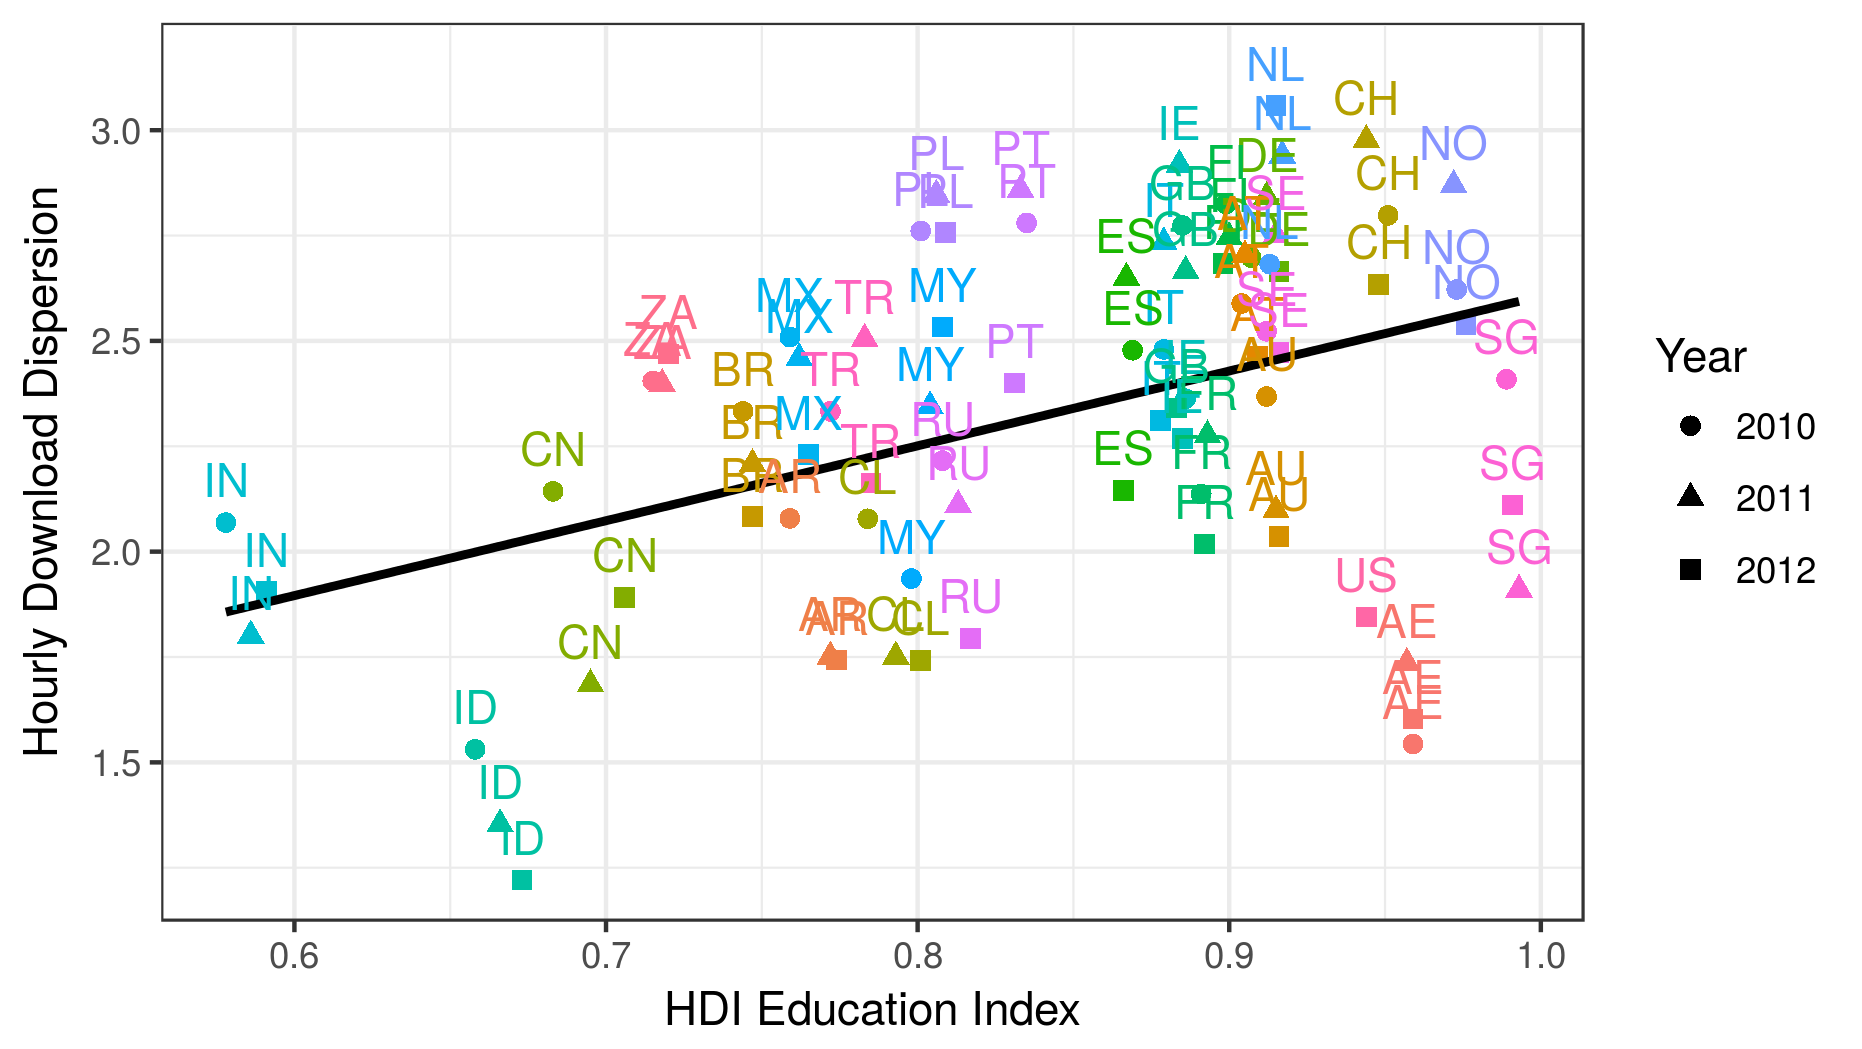
\includegraphics[width=\linewidth]{HDI_hourlyDispersion_education.png}
% \caption[HDI Hourly Dispersion]{HDI 24-hour to HDI Education $\sigma$}
% \end{figure}

% \begin{figure}[h!]
% 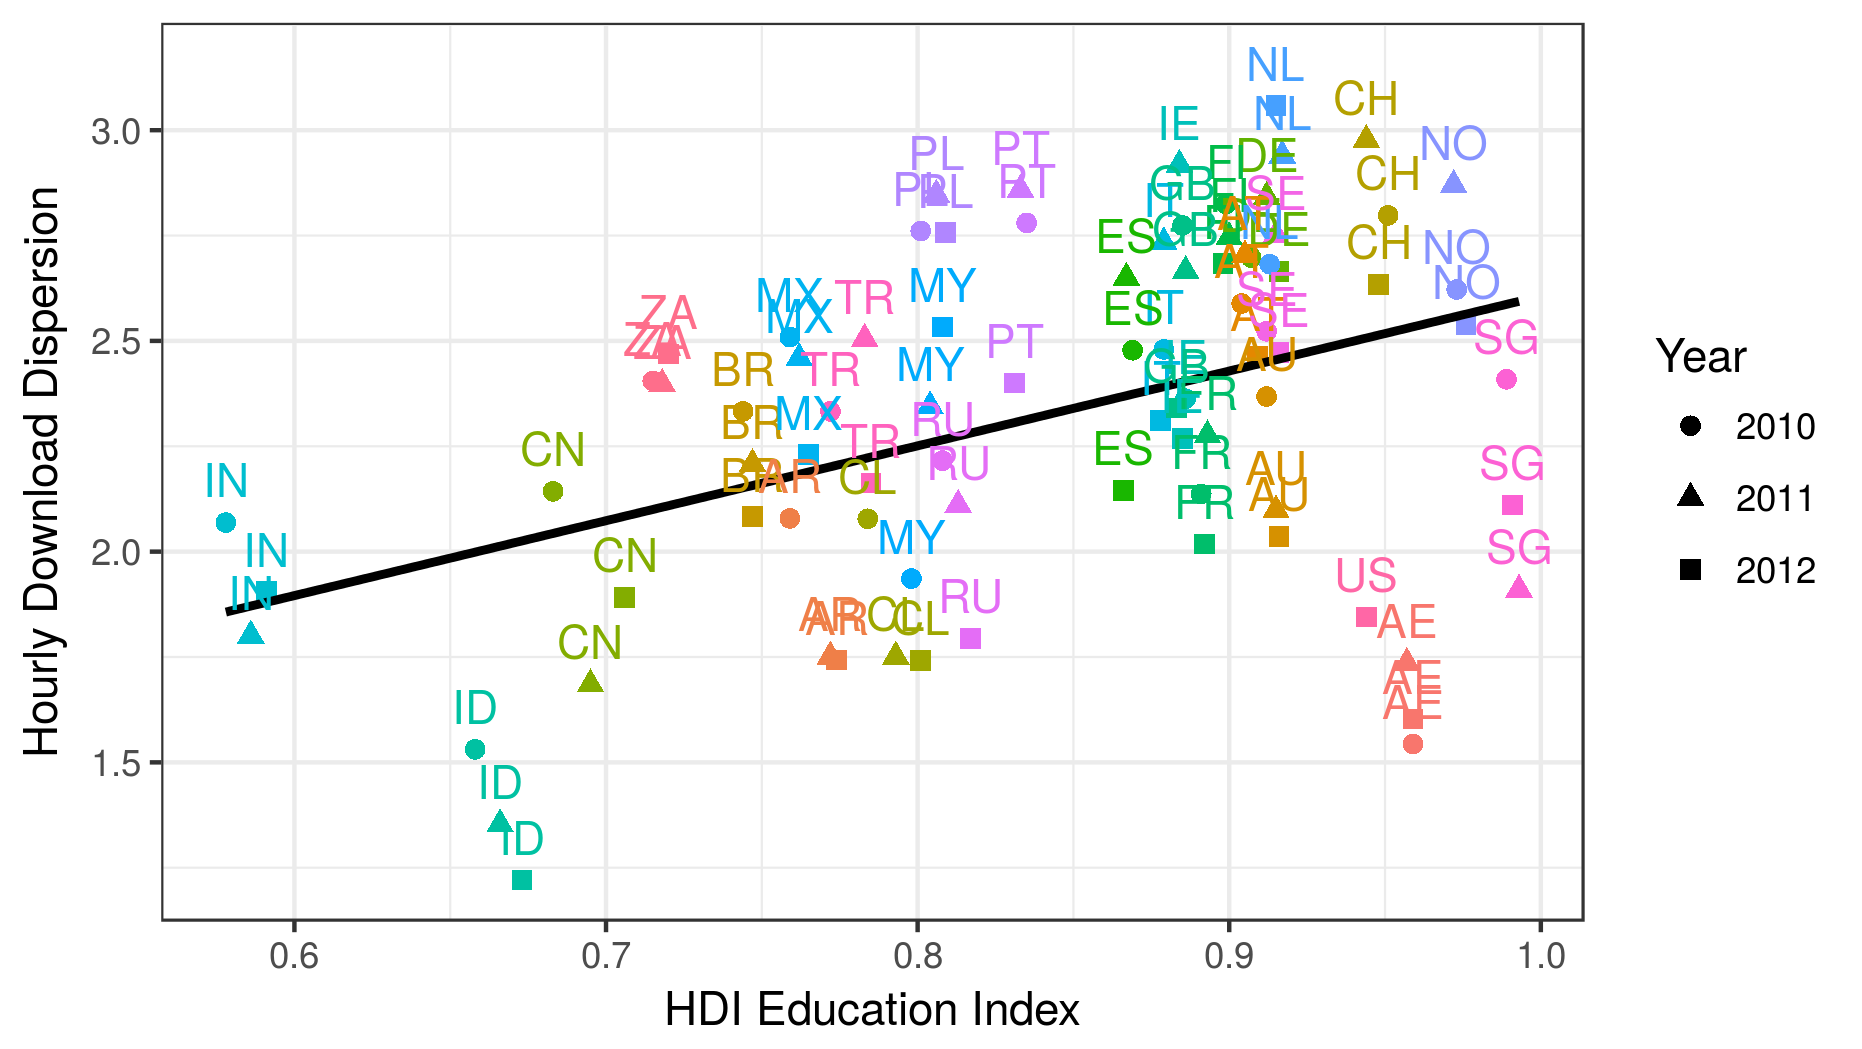
\includegraphics[width=\linewidth]{HDI_weeklyDispersion_income.png}
% \caption[HDI Weekly Dispersion]{HDI 7-day to HDI Income $\sigma$}
% \end{figure}

%%%% MOBILE PHONE DATA WITHOUT INTERACTIONS
% \begin{table}[h!]
% \centering
% \begin{tabular}{|c|c|c|c|}
% \hline
% \textbf{HDI Statistic} & \textbf{t-value} &  \textbf{r} & \textbf{p} \\
% \hline
% Income & $-2.793$  & $-0.48$ & $0.0097^{**}$ \\
% \hline
% Education & $-2.160$ & $-0.39$ & $0.0401^*$ \\
% \hline
% Health & $-0.944$ & $-0.18$ & $0.3537$ \\
% \hline
% \end{tabular}
% \caption[Proportion of Mobile-Phone Use and HDI]{Pearson product-moment correlations coefficients significant for all indices except Health. 3 years of HDI statistics included (2010-12; n=87). Individual linear correlations find patterns, but multiple linear regressions with interaction effects did not.}
% \end{table}

\paragraph{Country-level Eclecticism.}
Based on the data available within Nokia DB, this thesis defines eclecticism heuristic as the degree of overall balance in downloaded genres across countries or users, and is formalized in Equation \ref{eq:country}. Eclecticism is calculated by counting every genre downloaded within a country. The top 10 downloaded genres are selected, and normalized to a proportion and $\sigma$ is calculated for this 10 element array. Higher values indicate less eclectic users or countries with less eclecticism, and lower values indicate more eclectic countries. Country-level eclecticism scores were calculated for every year and country in the Nokia DB. Figure \ref{fig:ecclec} illustrates eclecticism as a stacked-bar graph.  Each bar is a country, and every colour stacked on a country represents proportion of downloads from one of 10 downloaded genres. For example, the orange bar for IN (India) is Bollywood, which  corresponds to approximately 40\% of all downloaded music by India in 2011. More eclectic countries have more equal representation of genres (i.e. for a country to be maximally eclectic, all ten bars should be close to 0.1).

First, individual linear regressions are conducted on \Gls{HDI} and closely related statistics found in the HDR (Table \ref{tab:hdi_lin_country}); additional metrics include school enrolment ratio (i.e. how many students were expected to enrol versus how many did), expected years of schooling for males and females, and acoustic features extracted through \Gls{GRAIL}. To determine if the iHDI is a more sensitive measure for analysis, two multiple linear regressions are conducted using country-level eclecticism with the components of the \Gls{HDI} and \Gls{iHDI} (Table \ref{tab:hdicomp}). Based on the sociological work described in Section \ref{sec:hdi}, it is hypothesized that education and income (indicators of class and status) should be negatively correlated with our measure of country-level eclecticism. 

\begin{equation}
\sigma_c = \left\{ p_g = \dfrac{g_c}{\sum\limits_{g=1}^{10} g_c}; g \in [1,10]  \right\}
\label{eq:country}
\end{equation}

Where:
\begin{description}\itemsep0em 
\vspace{2em}
\item[$g$] = Genre
\item[$u$] = Country
\item[$\bar{\sigma_c}$] = Standard Deviation of top-10 genre proportions in a given country
\item[$p_g$] = Proportion of downloads ($p$) for a top-10 genre
\item[$g_c$] = Count of downloaded genre in a country
\end{description}

\begin{figure}[h!]
\centering
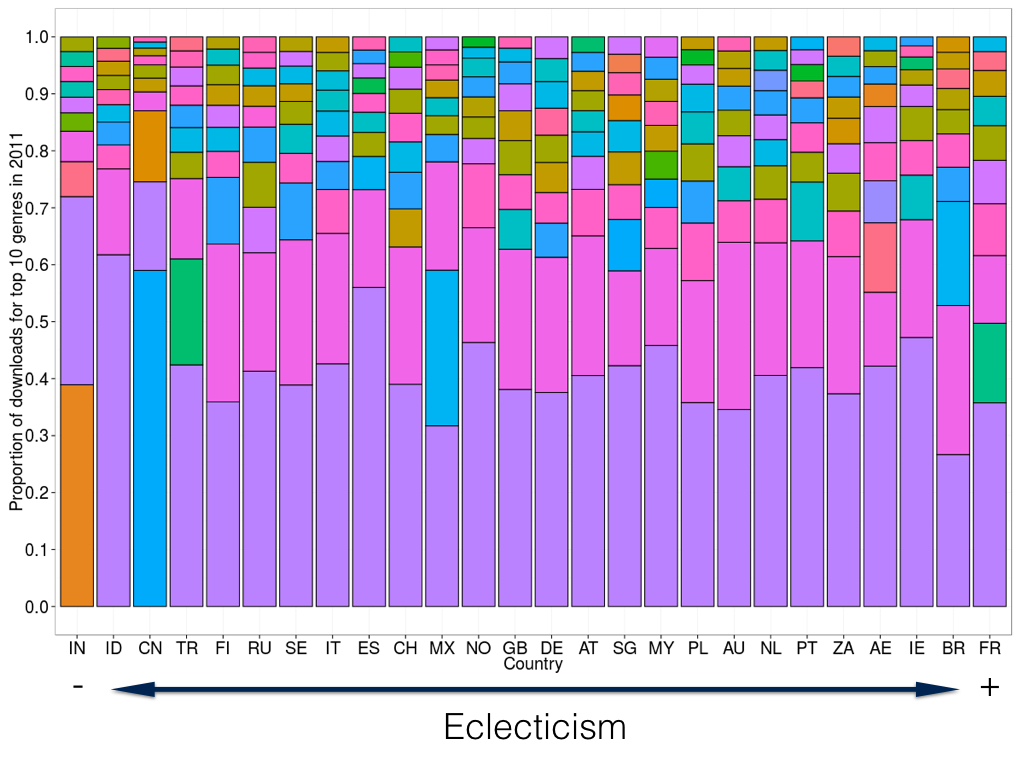
\includegraphics[width=\linewidth]{hdi_eclectic}
\caption[Eclecticism and HDI by country]{Proportion of top-10 downloaded genres by country in 2011. Genres represented by different colours. Countries are order by least to most eclectic based on the calculation described in Equation \ref{eq:country}}
\label{fig:ecclec}
\end{figure}

Table \ref{tab:hdi_lin_country} includes all significant individual correlations found during preliminary analysis. Income, education, and all but one additional measure of education are significantly correlated in the direction we expect. Effect sizes are relatively weak ranging from $r^2 = 0.0729-1.591$. Significant correlations generally support the hypothesis that education and income influence music preferences. As expected, no correlation was found for eclecticism and \Gls{HDI}'s health index. The direction of correlation for gross primary enrolment ratio is opposite to what was expected. This may be due to how enrolment ratios are calculated; determining expected enrolment for initial entry into education is much harder to track than at later years due to parents deciding to delay enrolment or inaccurate birth reporting.

\begin{table}[h!]
\centering
\begin{tabular}{|c|c|c|c|c|}
\hline
X & Y & N & P & R \\
\hline
\Gls{HDI} & Top 10 SD & 87 & 0.0127* & -0.27 \\
\hline
Income Index & Top 10 SD & 87 & 0.0093** & -0.28 \\
\hline
Education Index & Top 10 SD & 87 & 0.0042** & -0.3 \\
\hline
Expected years of schooling; female & Top 10 SD & 70 & 0.0016** & -0.37 \\
\hline
Expected years of schooling; males & Top 10 SD & 70 & 0.0018** & -0.37 \\
\hline
Gross primary enrolment ratio & Top 10 SD & 70 & 0.0098** & 0.3 \\
\hline
Gross secondary enrolment ratio & Top 10 SD & 69 & 0.0166* & -0.28 \\
\hline
Gross tertiary enrolment ratio & Top 10 SD & 69 & 0.001*** & -0.39 \\
\hline
\end{tabular}
\caption[Country-level Linear Regressions]{Individual Linear Regressions for country-level eclecticism measure.}
\label{tab:hdi_lin_country}
\end{table}

Two multiple linear regressions were run to determine whether \Gls{iHDI} is more sensitive to use with measures of human behaviour like music eclecticism. At the time of collection from the \Gls{API} \Gls{API}, only one year of iHDI data (2012) was available for analysis. Consequently, this analysis compared multiple linear regression models for 2012 \Gls{HDI} and iHDI data only. Overall, iHDI accounted for more than twice as much variance as the \Gls{HDI} model ($r^2=0.09961-0.1934$, respectively); significant main effects were found for the income and education indices as expected. Significant two-way interactions were found between income/life expectancy indices ($t=-2.166, p = 0.0468$), and education/income indices ($t=2.22,p=0.0422$). Marginal two- and three- way interactions were found for education/health ($t=2.21, p=0.0992$) and education/health/income ($t=2.072,p=0.056$). Although significant and marginal interaction effects were found for all indices, these results support past research examining demographic information including education and employment to global music preferences \cite{leblanc1999effect,north2013musical}. Although interactions are consistent with previous literature, complex effects make it difficult to confirm the nature of the relationship as described in the hypothesis. In the context of this work, it is unclear which, or how, each index is influencing eclecticism.  No significant main effects or interactions were found using \Gls{HDI}, suggesting that the \Gls{iHDI} may be more appropriate to use for analyzing global music preferences. Additional methodological weaknesses should be considered: although the \Gls{iHDI} generally performs better than the \Gls{HDI} for this analysis, our sample size is relatively low and does not span across many years. Another weakness is that country-level eclecticism is very high-level, and does not account for individual user differences. In light of this considerations, a user-level eclecticism calculation is derived and compared to \Gls{HDI} data for regression analysis.

\begin{table}[h!]
\small
\centering
\begin{tabular}{|l|c|l|l|l|}
\hline
\textbf{X} & \textbf{Y} & \textbf{Score} & \textbf{$p$} & Adjusted $r^2$  \\
 \hline
\makecell[l]{\\\\1) \Gls{iHDI} Income Index\\2) \Gls{iHDI} Education Index\\3) \Gls{iHDI} Health Index} & Country SD & \makecell[l]{\\F(3, 24) = 2.998\\t(26) = 2.556\\t(26) = -2.092\\t(26) = -1.002} & \makecell[l]{\\p < 0.0523\\1) p = 0.018*\\2) p = 0.04823*\\3) p = 0.327} & 0.1934 \\
\hline
\makecell[l]{\\\\1) \Gls{HDI} Income Index\\2) \Gls{HDI} Education Index\\3) \Gls{HDI} Health Index} & Country SD & \makecell[l]{\\F(7, 20) = 1.427\\t(26) =  0.62\\t(26) = 0.162\\t(26) = -0.046} & \makecell[l]{\\p = 0.2494\\1) p = 0.542\\2) p = 0.912\\3) p = 0.964} & 0.09961 \\
\hline
\end{tabular}
\caption[Multiple Linear Regression Comparison Analysis (\Gls{HDI} and \Gls{iHDI})]{Multiple Linear Regression Analysis using \Gls{HDI} to \Gls{iHDI} statistics and country-level eclecticism. Results suggest that iHDI may be a more sensitive statistic for evaluating global consumption trends.}
\label{tab:hdicomp}
\end{table}

\subsubsection{Analysis 2: User-level} \label{sec:eclectic}
User-level eclecticism, Equation \ref{eq:user} was calculated in a manner similar to Equation \ref{eq:country}. However, rather than calculating a single $\sigma$ per country, an exhaustive calculation is conducted for every user. User-level eclecticism is determined by taking a median eclecticism value from every user within a country. Values of zero are added to the the vector when a user has less than 10 genres in their download history.

\begin{equation}
\tilde{\sigma_c} = \left\{ p_g = \dfrac{g_u}{\sum\limits_{g=1}^{10} g_u}; g \in [1,10]  \right\}
\label{eq:user}
\end{equation}

Where:
\begin{description}\itemsep0em 
\vspace{2em}
\item[$g$] = Genre
\item[$u$] = User
\item[$\tilde{\sigma_c}$] = Median SD of top-10 genres for all users in a given country
\item[$p_g$] = Proportion of downloads ($p$) for top-10 genres in a user's collection
\item[$g_u$] = Count of downloaded genre in a user's ($u$) collection
\end{description}

As previous, individual linear regression analysis was first conducted using the user-level eclecticism measure with the \Gls{HDI} and other closely related statistics; additional metrics are identical to those used in country-level analysis. For a comprehensive list of HDR metrics, see Appendix \ref{tab:hdr}. Significant correlations are included in Table \ref{tab:hdi_lin_user}. Individual correlations reveal similar and stronger relationships than found in the country-level analysis of Table \ref{tab:hdi_lin_country}. Of note, a new significant correlation was found for the valence acoustic feature, and gross primary enrolment ratio is no longer significant. As described in Section \ref{sec:nokia}, valence is a perceptual estimation of a tracks positive/negative affect. Lastly, a multiple linear regression was conducted and compared to the results of Table \ref{tab:hdi_mlr_user}. A significant overall effect was found ($F(7,20) = 2.259, p=0.00482$), and a significant main effect was found for the health index.  However, a significant 2-way interaction was found between health/education indices ($t=-2.257, p=0.0354*$). The overall effect size using user-level eclecticism accounted for three times more variance than the country-level method.

\begin{table}[h!]
\centering
\begin{tabular}{|c|c|c|c|c|}
\hline
X & Y & N & P & R \\
\hline
\Gls{HDI} & Median SD & 28 & 0.0383* & -0.39 \\
\hline
Income Index & Median SD & 28 & 0.0097** & -0.48 \\
\hline
Education Index & Median SD & 28 & 0.0401* & -0.39 \\
\hline
Combined Enrolment both sexes  & Median SD & 20 & 0.0237* & -0.5 \\
\hline
Gross Primary Enrolment Ratio & Median SD & 21 & 0.0248* & 0.49 \\
\hline
Gross Tertiary Enrolment Ratio & Median SD & 20 & 0.0076** & -0.49 \\
\hline
Average Valence & Median SD & 28 & 0.0153* & -0.45 \\
\hline
\end{tabular}
\caption[Individidual Linear Regressions]{Individual Linear Regressions for user-level eclecticism measure.}
\label{tab:hdi_lin_user}
\end{table}

\begin{table}[h!]
\centering
\begin{tabular}{|l|c|l|l|l|}
\hline
\textbf{X} & \textbf{Y} & Score & \textbf{$p$} & \textbf{$r^2$}  \\
 \hline
\makecell[l]{\\\\1) \Gls{HDI} Income Index\\2) \Gls{HDI} Education Index\\3) \Gls{HDI} Health Index} & User SD & \makecell[l]{\\F(7, 20) = 2.259\\t(27) = 0.955\\t(27) = 1.962\\t(27) = 2.118} & \makecell[l]{\\p = 0.04482*\\1) p < 0.351\\2) p = 0.0638\\3) p = 0.0469*} & Adjusted: 0.2919 \\
\hline
\end{tabular}
\caption[User-level Eclecticism Multiple Linear Regression]{Multiple linear regression model using user-level eclecticism value. A two-way interaction between health and education (t=-2.257 p=0.0354)}
\label{tab:hdi_mlr_user}
\end{table}


% \begin{figure}[h!]
% \centering
% 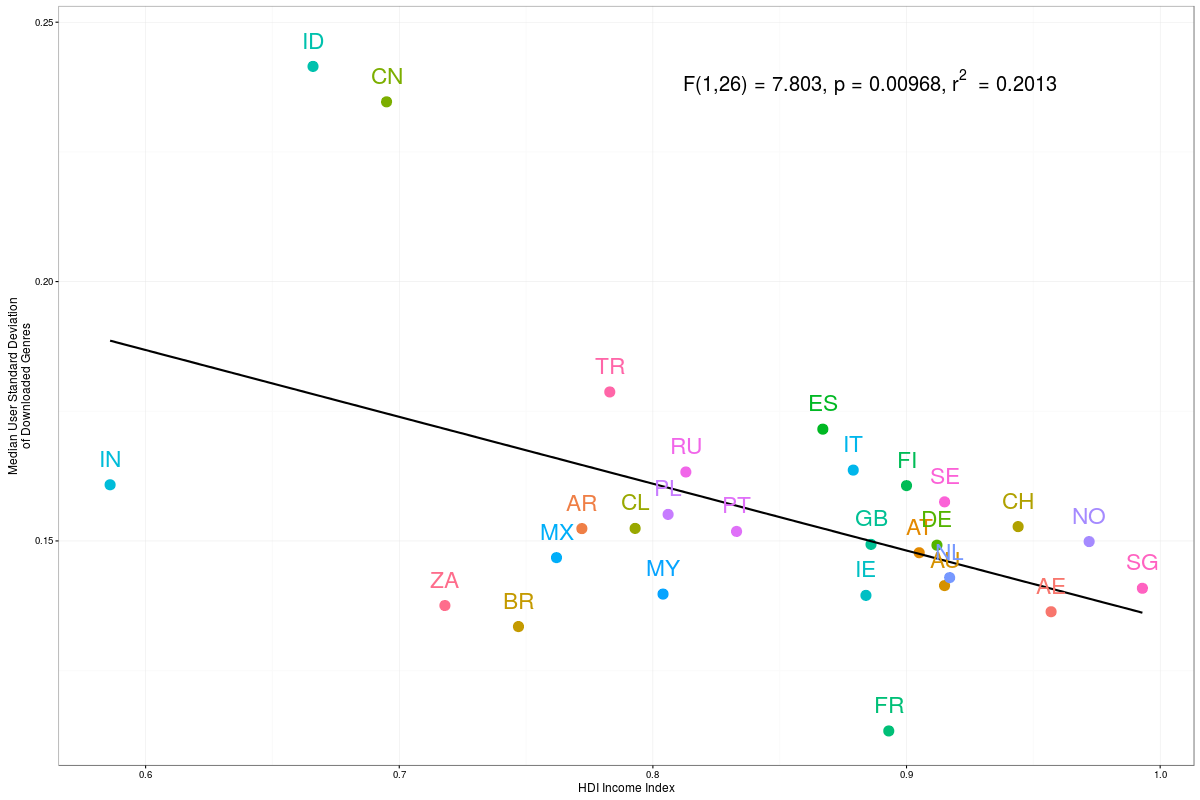
\includegraphics[width=\linewidth]{hdi_income}
% \caption[Eclecticism and HDI Income Index by country]{Scatter plot and linear regression for Income index of HDI against user-level eclecticism ($c_e$).}
% \end{figure}


% \subsubsection{Analysis 3: Gender Equality and Artist Preference}
% A final exploratory analysis exploiting the linkage from MusicBrainz to \Gls{GRAIL} was considered using artist demographic information. 20,000 artists are enriched with performer gender information. A simple calculation was derived (Equation \ref{eqn:asr}) to explore whether consumption of artists by sex is moderated by indices found in the HDR.

% \begin{equation}
% ASR = \dfrac{C_M}{C_F}
% \label{eqn:asr}
% \end{equation} 

% where:
% \begin{description}\itemsep0em 
% \vspace{2em}
% \item[$C$] = Country
% \item[$C_M$] = Total downloads for male artists in a given country
% \item[$C_F$] = Total downloads for male artists in a given country
% \end{description}

% \begin{table}[h!]
% \centering
% \begin{tabular}{|l|c|l|l|l|}
% \hline
% \textbf{X} & \textbf{Y} & Score & p & r2  \\
%  \hline
% \makecell[l]{\\\\1) HDI Income Index\\2) HDI Education Index\\3) HDI Health Index} & ASR & \makecell[l]{\\F(7, 20) = 2.259\\t(27) = -3.265\\t(27) = -2.764\\t(27) = -2.59} & \makecell[l]{\\p < 0.00453**\\1) p < 0.00388**\\2) p = 0.01196*\\3) p = 0.01748*} & Adjusted: 0.4208 \\
% \hline
% \end{tabular}
% \caption[Artist Sex Ratio Eclecticism Multiple Linear Regression]{2- and 3-way interactions between between all factors}
% \label{tab:hdi_mlr_artist}
% \end{table}

% \begin{itemize}
% \item  Calculated the Mean Artist Sex Ratio (ASR) proportion of times a downloaded artist was male/female for that country. 
% \item Collected male/female artist download counts for each country and calculated the ratio of females to males in downloads. (value closer to 1 = higher female representation) 
% \item Calculated average artist ratio for each country and compared to HDI 2011 results
% \item ASR associated with tempo, and HDI income, but no other features or indices
% \end{itemize}


\section{General Discussion}
Using an interdisciplinary approach, Section \ref{sec:grail} enriched and validated a large corpus of digital music metadata for CogMIR research; using this resource, Section \ref{sec:analyses} examined two topics relevant to MIR and cognitive psychology, which to some extent, addresses methodological concerns within both fields. However, some limitations remain. A common issue with "big data" resources concerns data consistency and reliability. This thesis, as well as a majority of MIR tasks, either rely on public user-contributed efforts \cite{swartz2002musicbrainz,sturm2012analysis} or private digital music platforms (see resource coverage in Section \ref{sec:grail}), both of which have been criticized for data reliability \cite{sturm2014state}. Public resources include inconsistent and/or controversial labeling, are absent of filters, and contain duplicate examples \cite{bogdanov2016cross}; furthermore, datasets fail to achieve similar classification accuracies using identical classification algorithms: cross-collection accuracies ranged from 6-53\% \cite{bogdanov2016cross}. Private resources also contribute to data faults: TuneCore,\footnote{\url{http://www.tunecore.com/}} an online digital music-distribution service, allegedly issued incorrectly formatted \Gls{ISRC}s without permission from the \Gls{ISRC}. As a result of TuneCore's alleged error, hundreds of thousands of songs were shown as being created in the British overseas territory of the Turks and Caicos Islands (ISO 3166-1-Alpha-2 country code TC). Given that TC has a population of only 33,000, this prodigious musical output is surely questionable and approximately one million \Gls{ISRC}s in \Gls{GRAIL} contain incorrectly assigned country code of TC. This inconsistency does not impact our linking process, but illustrates how industry-standard data can be affected by improper data practices. The intention of \Gls{GRAIL} was to address these issues by including filter procedures into the linking architecture, and motivate future work by making the codebase public; however, it does not fully alleviate the problem. Cooperation from the MIR community in the form of data access as well as technical and monetary support will be vital in order to achieve music-data accuracy.

Other measures of variance such as the Gini coefficient, $g$, should also be considered for deriving behavioural differences such as eclecticism from users. For example, the Gini coefficient is a measure of inequality traditionally used to evaluate income inequality, but has more recently seen applications in biology \cite{weiner1984meaning}, genetic expression \cite{kirchman2010structure}, and social psychology \cite{kumar2014detecting}. It is calculated (Equation \ref{eq:gini}) by taking the mean absolute difference divided by the average, and normalized for scaling. Given that our current version of eclecticism takes the standard deviation of a cumulative distribution of proportions (see Equation \ref{eq:country}), the Gini coefficient may be a more sensitive measure for determining inequalities in a user's genre preference and should be considered.

\begin{equation}
g = \dfrac{\sum\limits_{i=1}^n \sum\limits_{j=1}^n |x_i-x_j}{2n \sum\limits_{i=1}^n}
\label{eq:gini}
\end{equation}

The framework used to determine testable user preferences from large datasets considers statistical learning to be a shared theoretical underpinning across topics. An additional benefit was that statistical learning is also a familiar topic within MIR, providing an area of shared research interest that is equally understood in different but important ways. Although statistical learning is discussed as a mechanism for preferences and behaviours, no statistical learning procedure was used during the analysis. This thesis decided to use more traditionally psychological analysis techniques in part due to novel use of large volumes of acoustic features derived from private companies for cognitive research. Some research supports the notion that statistical learning is important in music perception and preference: EEG mismatch negativity is stronger when musicians hear musical violations in their genre of expertise \cite{brattico2009neural,Tervaniemi2014}. Although high-level acoustic features were used in this thesis, low-level features extracted in short windows of time are available for each track. Future work should include examining how statistical learning influences the perception and preference of acoustic features in short time intervals.

The algorithms responsible for Spotify's acoustic features are proprietary, and therefore not publically available. Although my primary aim was to investigate and record the presence of musical-feature influence, I was unable to assess in detail which specific acoustic elements were responsible for my findings. Which frequency bands within an X-head’s main genre, for example, have in general a greater influence on their other genres? Which components of Acousticness are present throughout an X-head’s download collection, and which are specific to the main genre? Moreover, and perhaps of greater import, as mentioned at the outset the psychological reality of acoustic features is, as yet, unquantified \cite{friberg2014using}. Although a feature like Valence may make “sense” to those who know and love music’s emotional power, its interpretation across listeners may be highly divergent. Another example, Danceability, is available in signal processing packages \cite{bogdanov2013essentia,Bogdanov2009FromMeasures} and open-access \Gls{API}s.\footnote{\url{https://developer.spotify.com/web-api/get-audio-features/}} It is derived from a combination of beat salience and consistency to derive a floating point for a song between zero and one \cite{streich2005detrended}. However, according to this definition the most danceable song should be a steady, metronomic-like pulse, which clearly does not capture the cognitive nuances of what makes music danceable. Perceptual experiences of music such as Danceability or Valence are undeniably more complex than these heuristic definitions and contribute to the inaccessibility of MIR for music cognition research \cite{aucouturier2012mel}. Acoustic features which focus on human perception \cite{friberg2014using} or user behaviour \cite{vigliensoni2016automatic}, rather than simplified or heuristic representations, are advantageous because they improve classification \cite{Chen2001,mckay2010evaluating,lippens2004comparison}, and provide more nuanced interpretability over acoustically or heuristically defined measures.

Section \ref{sec:leaky_anal_3} found little variation between acoustic features across genres in the Spotify library. Given that hundreds of acoustic features have been derived and used in a variety of MIR tasks, in recent years relatively small gains in accuracy have been made  \cite{sturm2014state}, suggesting possible ceiling effect using acoustic-only analysis. As a result, MIR's growing interest in using psychologically derived behaviours with the aim of improving predictive accuracy is not surprising \cite{lee2004survey}. Many features can be extracted from a piece of recorded sound. However, some acoustic features, like danceability, may not be wholly represented in the acoustic signal. These features can be considered inherently psychological features \cite{friberg2014using}. The process in Section \ref{sec:hdi} of deriving the psychological feature for eclecticism from consumption and demographic data, and providing an experimental means to determine its efficacy provides a framework to explore other types of consumption behaviours. Future work should include testing new behaviours (four described in Section \ref{sec:future}) relevant to CogMIR research. Additionally, directly testing the perceptual efficacy of acoustic features in an controlled laboratory should be considered. Appendix \ref{sec:mental} includes more future work using \Gls{GRAIL} as a research proposal which is beyond the scope of this work's research focus. This work describes a digital journaling application which uses music and natural language processing, and psycholinguistics as a way of informing current mental health states.

\subsection{Future Directions}\label{sec:future}
% The more information people have, the more they go on mood.  are they going more on mood rather than personality when given more information based on the AIM model. How do complex situations influence things (relying on mood)
\subsubsection{User Acoustic Behaviours}
Because there is a low degree of variance across high-level acoustic features for music, user behaviour may be more appropriate for a variety of MIR classification tasks \cite{vigliensoni2016automatic}. Diversity can be measured in many ways. It could represent preferences for a variety of genres (i.e. eclecticism), or a preference for music that is more or less mainstream (i.e. mainstreamness \cite{vigliensoni2016automatic}). Additionally, temporal patterns of music consumption differ across national and demographic boundaries \cite{molteni2003consumption,woolhouse2013work}. Users with differing musical preferences exhibit different patterns of regular downloading based on differences in personality traits such as openness to experience\cite{rentfrow2003re}. However, regularity in consumer patterns may be under-reported because users tend to repeat purchasing habits regardless of intent \cite{ji2007purchase}. Global patterns of genre and temporal consumption are relatively unexamined within both music cognition and MIR. Alongside our measure of eclecticism (Section \ref{sec:eclectic}), we propose four new behavioural features and outline their calculations: overall regularity, periodic regularity, adventurousness, and volume.

Adventurousness can be defined for each user by considering the average popularity for each track downloaded by a user in the Nokia DB. The total number of times each track was downloaded was pre-computed as a measure of overall song awareness. In general, music consumption generally follows an Zipf-like distribution of growth with respect to downloads and popularity (see Section \ref{sec:nokia}); Appendix \ref{app:adv} describes a method and example for calculating adventurousness. Volume measure of user engagement that considers traditional measures like play count \cite{Chen2001}, but also takes into consideration aspects of temporality. For example, two users who download 100 songs should not be considered equal consumers if user 1 downloaded 1 song over 100 days or 100 songs or 1 day; Appendix \ref{app:vol} provides an equation for calculating user volume. Overall regularity measures the degree of day-by-day download activity. Appendix \ref{app:oreg} illustrates how overall regularity is calculated for two users. Periodic (7-day) regularity refers to the degree of regular behaviour across the week. Measuring overall regularity may find general patterns of behaviour across a users entire history, but miss regularity in specific, weekly intervals; Appendix \ref{app:preg} illustrates periodic regularity for one user with three weeks of download behaviour. 

\section{Closing Remarks}
In summary, this thesis explored three topics relevant to cognitive science and MIR research, and to some extent, attempts to address issues with both.  The first topic explored the current state of music metadata consistency. Using a large metadata catalogue of digital tracks provided by Nokia, Section \ref{sec:grail} enriched an already expansive set to include an diverse set of music metadata which enabled the analysis. Although the purpose of this topic was to inform cognitive research, and was primarily methodological in nature, it represents an novel contribution to MIR and future cognitive research by focusing on metadata linking and validation efforts. To encourage further efforts, Section \ref{sec:grail} presents code-base and linked data as an open-access \Gls{API}.\footnote{\url{http://api.digitalmusiclab.org/}}

Topic two regarding acoustic features and genre preference found strong evidence of influence with respect to users’ consumption of multiple styles of music; clear relationships emerged between the features of X-heads’ main and secondary genres. This effect was found to be stronger for some features than others, most noticeably Speechiness, Danceability, and Loudness, and more pronounced in certain subgroups, such as Metal-heads, Jazz-heads and Dance-heads. While the reasons for differential effects within features and X-heads is unknown, two probable, independent causal mechanisms were suggested to account for general main-to-secondary genre influence. First, personality creates an overarching psychological framework in which certain factors, such as openness and agreeableness, guide musical preference, irrespective of genre; some personality factors may be linked to specific acoustic features. Second, via statistical learning, listeners extract the acoustic regularities of various musical features, which in turn influence the creation of musical preferences beyond established styles and/or genres. Of course, these mechanisms need not be mutually exclusive, but may serve to reinforce one another. Attempts, therefore, to tease apart the effects of personality and statistical learning could prove to be difficult, although paradigms in which these factors are independently manipulated might settle the issue of personality versus statistical learning conclusively. 

Topic three explored the extent to which user behaviours defined from social psychological research could be used to determine trends in global music preference. Extending past research examining temporal aspects of human consumption \cite{woolhouse2013work} and human development, this work examined whether a new feature, eclecticism, could be derived and validated using a more rigorous hypothesis and analysis. As predicted, significant correlations were found for income and education measures provided by the \Gls{UN}. Furthermore, this analysis determined that user-level eclecticism and inequality-sensitive derivatives of the \Gls{HDI} were significant in a multiple linear regression using country-level eclecticism and the \Gls{iHDI}. Main effects for the multiple linear regression model included income and education, also as predicted. Although the method of deriving eclecticism from digital consumption data in all likelihood will not be the definitive measure over time, the theoretical underpinning and process of validation is novel and contributes to powerful, but relatively unexplored data sources in the cognitive sciences. 

The topics explored in this work has a variety of implications future music cognition research. This work uses utilizes enriched metadata from multiple open-access big data research is uncommon in cognitive sciences, but is quickly becoming an attractive alternatives to traditional methods; the amount of data and relative ease of computational analysis enables research to be executed quickly with a high degree of external validity. By addressing significant concerns of data integrity commonly voiced by the psychological community and providing a resource which attempts at alleviate them is novel; \Gls{GRAIL}'s validation procedures contribute to the groundwork for comprehensive music metadata collection and cleaning. While it is intuitive that human preference for new genres may be informed by features commonly found in past preferences, little work has been able to address the questions highlighted in Analysis 1 concerning which, and to what degree, these features are motivating music choice. Furthermore, this information informs MIR research regarding which extraction algorithms are sensitive to differences across genres and users. Lastly, the work in Analysis 2 implies that that user features may be more valuable than acoustic features for MIR classification tasks  and provides additional legitimacy to topics in social psychological research on eclecticism examining the extent to which socioeconomic factors influence music consumption behaviours across national boundaries.

A primary motivation of this thesis was to undertake interdisciplinary research in MIR and cognitive science, capitalizing on the advantages of each while minimizing the concerns of both. While commonplace for technologically driven research, large and diverse datasets like the Nokia DB are rare within cognitive psychology. The relative rarity of these kinds of resources is, in part, due to methodological concerns voiced by more traditional psychological practices \cite{aucouturier2013seven}, and weak applications of established psychological findings on human music preception \cite{krumhansl1997exploratory,aucouturier2012mel}. The extent to which the research contributions generated by this thesis address these concerns will be determined over time; it is the author's hope that the resources and methods made public by this endeavour eases future interdisciplinary research initiatives and provides a stepping stone for psychology to enter into CogMIR research.

\newpage

\bibliographystyle{ieeetr}
\bibliography{thesis,stigma}

\newpage
\section{Appendix\label{sec:appendix}}
%%% ADD \Gls{GRAIL} AND FRONTIERS PAPER
\subsection{Nokia DB Genre List}
\begin{table}[h!]
\title{Exhaustive Genre List:}\\
African Ethnic/Traditional, Afrikaans, Ambient/New Age, Asian, Australian Music, Bengali, Bhojpuri, Blues, Bollywood, Cancion de autor, Cantonese Pop, Chinese Original, Christian/Gospel, Christmas, Classic Arabic/Tarab, Classical, Comedy, Country and Western, Dance, Dangdut, DeutschPop, Devotional, Easy Listening/Oldies, Electronica, Flamenco, Folk/Roots, French Variety, Ghazal, Greek, Gujarati, Hindustani Classical, Indie/Alternative, Indipop and Remix, Instrumental, Irish Music, Iskelda, Islamiyat, Italiana, Jazz, Keroncong, Khaleeji, Kids/Novelty, Latin Music, Malayalam, Mandarin Pop, Marathi, Metal, Nederlandstalig, Oriental Pop, Other, Pop, Punjabi, Punk, Rap/Hip Hop, Reggae, Regional/Others, Rock, Schl{\"a}ger, Shanson, Soul/R 'n' B/Funk, Soundtracks/Musicals/Theatre, South Devotional, Spanish pop rock, Spoken Word, Tamil, Telugu, and World.
\caption[Complete Nokia DB Genre List]{Exhaustive list of all genres included in Nokia DB.}
\end{table}

\subsection{User Distribution Statistics}
\begin{table}[h!]
\small
\centering
\csvreader[tabular=|c|c|c|c|c|c|,
  table head=\hline \bfseries Xhead & \bfseries Average & \bfseries Mode & \bfseries Standard Deviation & \bfseries Skew & \bfseries Kurtosis \\\hline,
  late after line=\\\hline]%
  {data/xheadCurveStats.csv}{}%
{\csvlinetotablerow}%
\caption[X-head Distribution Summary Table]{X-head distribution summary statistics}\label{tab:xheadDist}
\end{table}

\subsection{Analysis 1: Supplemental Information}
\begin{figure}[h!]
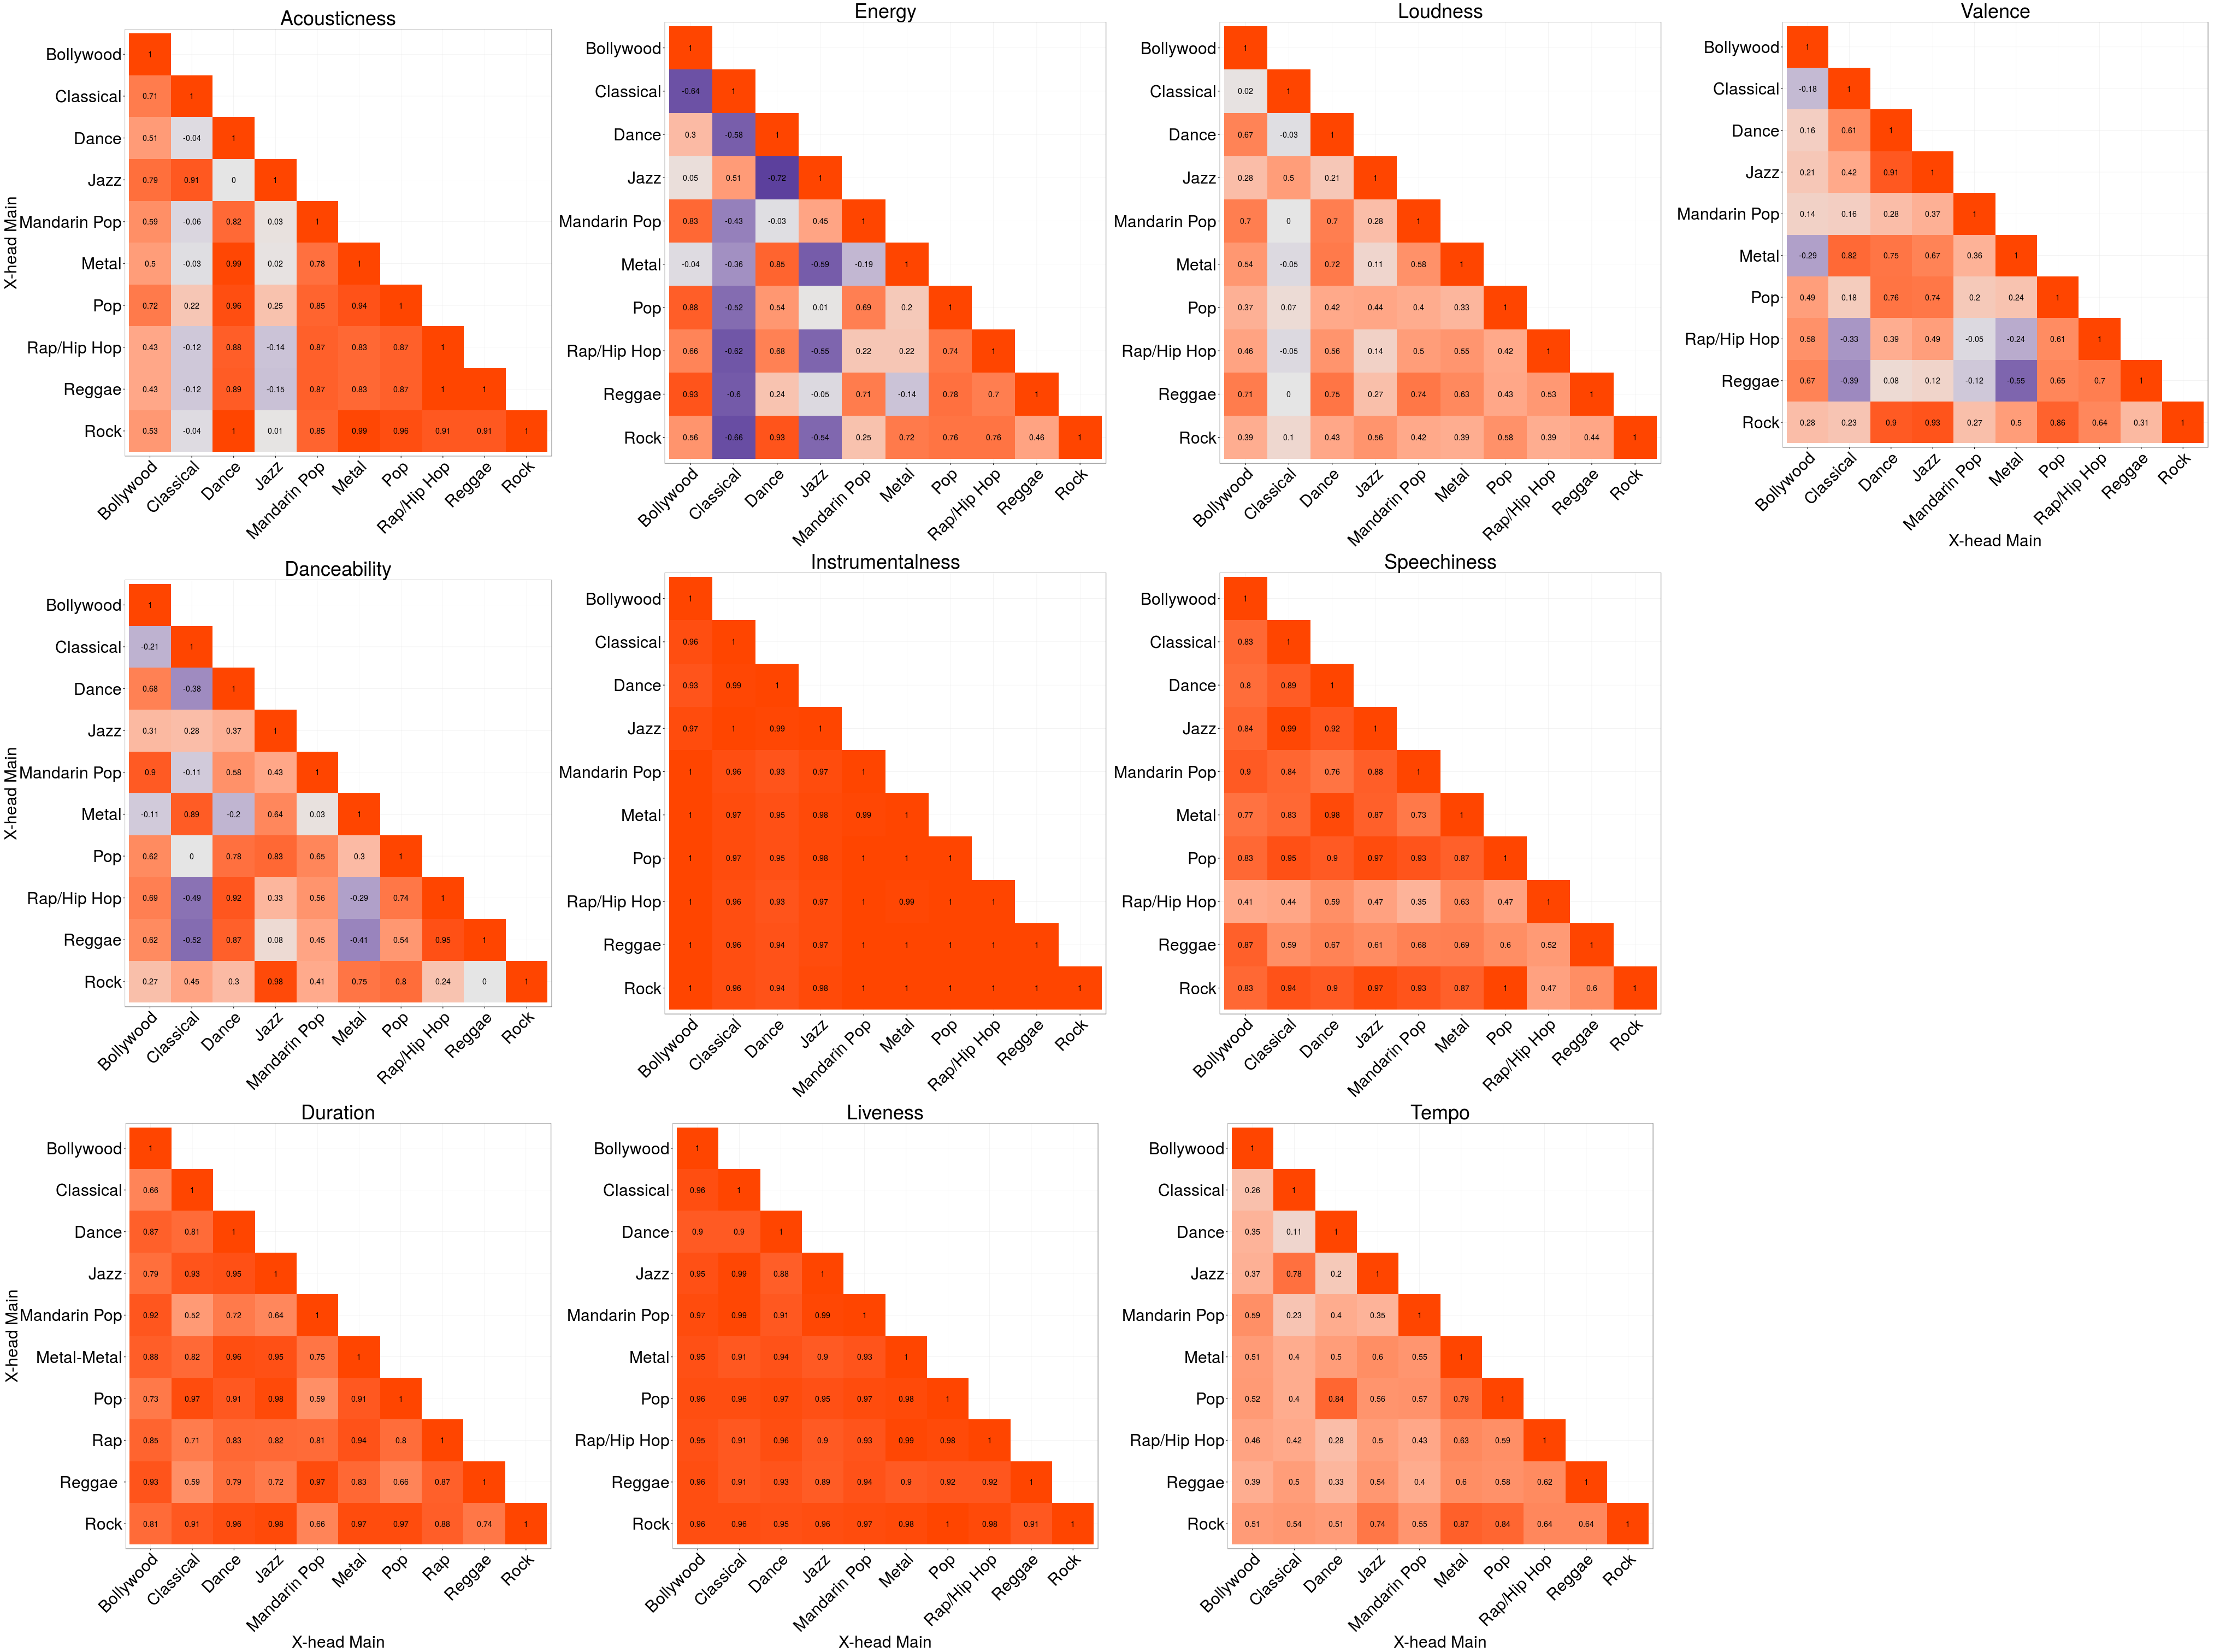
\includegraphics[width=\linewidth]{correlationSupplemental}
\caption[Correlation Supplemental]{Correlation Matrices for all features}
\end{figure}

\begin{figure}
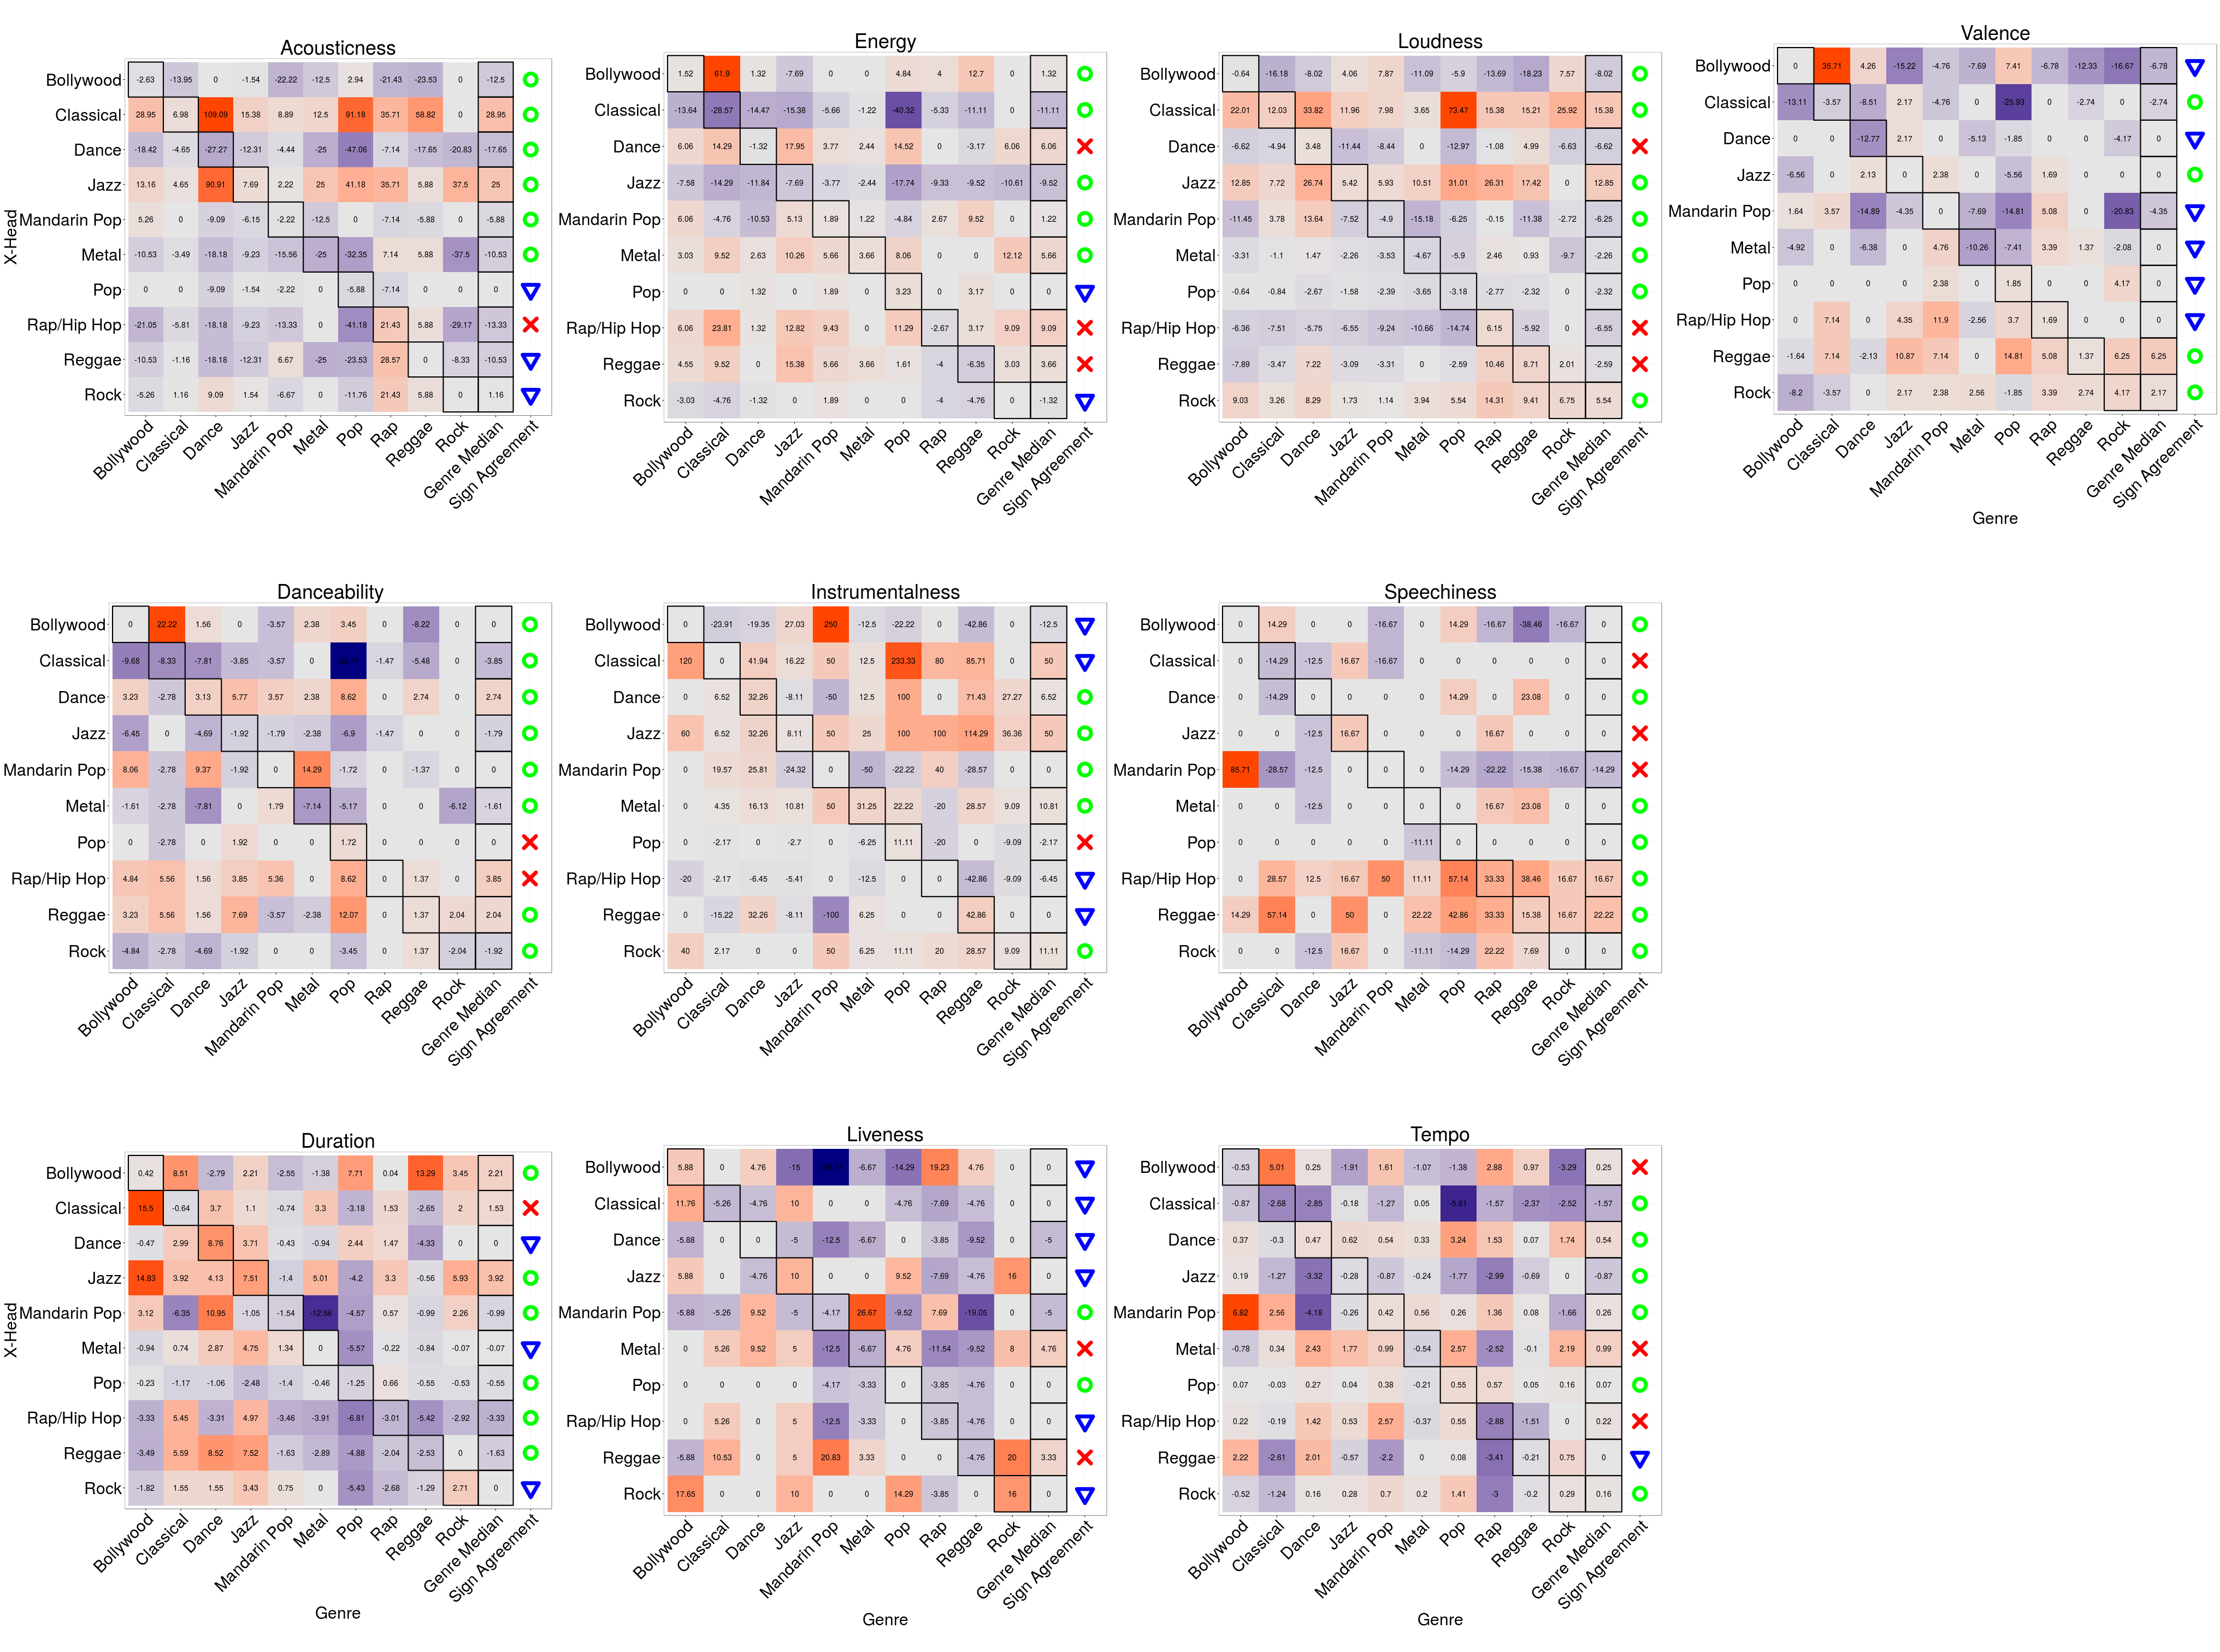
\includegraphics[width=\linewidth]{leakySupplemental}
\caption[Leaky Supplemental]{Leaky Features Matrices for all features}
\end{figure}

\begin{table}[h!]
\small
\begin{longtable}{|c|c|c|c|c|c|}
\hline
\textbf{X-head} & \textbf{Feature} & \textbf{JT value} & \textbf{JT p-value} & \textbf{KT value} & \textbf{KT p-value} \\ \hline
Rap/Hip Hop & Speechiness & 4420833.225 & 0 & 0.12491392 & 5.08E-21 \\ \hline
Easy Listening/Oldies & Speechiness & 3483741.525 & 1.43E-30 & -0.148123249 & 2.12E-32 \\ \hline
Easy Listening/Oldies & Acousticness & 3509958.405 & 1.18E-27 & -0.140552878 & 2.64E-29 \\ \hline
Easy Listening/Oldies & Energy & 4326665.495 & 7.26E-13 & 0.095272168 & 1.58E-13 \\ \hline
Easy Listening/Oldies & Loudness & 4323052.59 & 1.15E-12 & 0.094302639 & 2.49E-13 \\ \hline
Classical & Loudness & 3702954.72 & 2.17E-08 & -0.085093698 & 9.04E-09 \\ \hline
Classical & Energy & 3706545.725 & 3.03E-08 & -0.084104458 & 1.27E-08 \\ \hline
Dance & Liveness & 4210263.695 & 3.41E-08 & 0.085957604 & 1.45E-08 \\ \hline
Easy Listening/Oldies & Liveness & 3457439.455 & 4.58E-08 & -0.073989712 & 1.87E-08 \\ \hline
Easy Listening/Oldies & Instrumentalness & 3452329.965 & 1.19E-07 & -0.075137635 & 5.78E-08 \\ \hline
Dance & Instrumentalness & 4210658.875 & 4.61E-07 & 0.086140214 & 2.46E-07 \\ \hline
Reggae & Energy & 3773462.645 & 1.67E-05 & -0.063703114 & 1.03E-05 \\ \hline
Reggae & Speechiness & 4201039.445 & 2.85E-05 & 0.059831632 & 1.75E-05 \\ \hline
Metal & Acousticness & 3769708.685 & 4.57E-05 & -0.06439462 & 3.09E-05 \\ \hline
Metal & Liveness & 4162542.96 & 0.000146414 & 0.06104769 & 0.000101317 \\ \hline
Metal & Instrumentalness & 4158687.675 & 0.000174479 & 0.059759437 & 0.000124271 \\ \hline
Dance & Loudness & 3802907.725 & 0.000470196 & -0.054276528 & 0.000346346 \\ \hline
Rap/Hip Hop & Tempo & 3792420.385 & 0.000600026 & -0.056716182 & 0.000477608 \\ \hline
Indie/Alternative & Danceability & 3795041.915 & 0.000626752 & -0.056934399 & 0.000479848 \\ \hline
Metal & Danceability & 3809333.595 & 0.000767723 & -0.053938317 & 0.000585056 \\ \hline
Rap/Hip Hop & Loudness & 3811668.515 & 0.000983393 & -0.050979958 & 0.000751357 \\ \hline
Classical & Danceability & 3799482.445 & 0.00111005 & -0.057267287 & 0.000914941 \\ \hline
Rap/Hip Hop & Energy & 3807555.425 & 0.001194797 & -0.052338623 & 0.000942086 \\ \hline
Pop & Loudness & 4176554.4 & 0.001366168 & 0.052823373 & 0.001071435 \\ \hline
Jazz & Instrumentalness & 4138031.56 & 0.002094058 & 0.046914829 & 0.001683323 \\ \hline
World & Loudness & 4126809.52 & 0.002310272 & 0.051064518 & 0.001893119 \\ \hline
World & Danceability & 4120797.03 & 0.002731817 & 0.049438012 & 0.002234467 \\ \hline
Jazz & Liveness & 4140682.89 & 0.003141327 & 0.047777196 & 0.00256336 \\ \hline
Easy Listening/Oldies & Mode & 1373230.74 & 0.003389393 & 0.047338072 & 0.002594141 \\ \hline
Rock & Loudness & 3837985.35 & 0.004482714 & -0.046008169 & 0.003747369 \\ \hline
Dance & Tempo & 4148610.84 & 0.005072021 & 0.046330913 & 0.00432647 \\ \hline
Reggae & Loudness & 3862190.335 & 0.008443676 & -0.037985968 & 0.006949752 \\ \hline
Metal & Valence & 3855420.78 & 0.010277592 & -0.04063668 & 0.008966439 \\ \hline
Dance & Acousticness & 3829994.22 & 0.012267716 & -0.04644522 & 0.011123995 \\ \hline
Metal & Energy & 4136202.535 & 0.014187845 & 0.040459403 & 0.0123767751 \\ \hline
Pop & Liveness & 3333950.37 & 0.019457481 & -0.039706259 & 0.017301732 \\ \hline
Pop & Instrumentalness & 3324721.405 & 0.019963691 & -0.042221331 & 0.018013182 \\ \hline
Rap/Hip Hop & Danceability & 4118192.445 & 0.020945384 & 0.037469885 & 0.018736737 \\ \hline
Mandarin Pop & Loudness & 4083001.82 & 0.025359759 & 0.034072809 & 0.022178097 \\ \hline
Metal & Speechiness & 4124863.955 & 0.026107106 & 0.03719727 & 0.023439102 \\ \hline
Indie/Alternative & Instrumentalness & 4048017.01 & 0.04031904 & 0.033406131 & 0.036238921 \\ \hline
Rap/Hip Hop & Liveness & 2392465.12 & 0.043350052 & -0.038637571 & 0.040514344 \\ \hline
Dance & Valence & 3873661.13 & 0.046940941 & -0.033883289 & 0.043581095 \\ \hline
Pop & Acousticness & 3883316.605 & 0.053402234 & -0.031996299 & 0.049285072 \\ \hline
Rap/Hip Hop & Instrumentalness & 2400866.635 & 0.054940394 & -0.036013261 & 0.051331202 \\ \hline
Rock & Valence & 4112147.94 & 0.055357385 & 0.033061069 & 0.05216693 \\ \hline
Rock & Instrumentalness & 3966354.31 & 0.061004966 & 0.03232337 & 0.056820527 \\ \hline
Indie/Alternative & Liveness & 4035347.78 & 0.068423033 & 0.029564819 & 0.063453665 \\ \hline
Pop & Energy & 4101348.62 & 0.070413574 & 0.03097653 & 0.066164627 \\ \hline
Rock & Liveness & 3963854.315 & 0.072977068 & 0.031477018 & 0.068418915 \\ \hline
Dance & Speechiness & 3898293.015 & 0.103202653 & -0.026821199 & 0.097596423 \\ \hline
\caption[Jonchkheere-Tersptra and Kendall-Tau-$\beta$ results]{Jonchkeere and Kendall-Tau-$\beta$ results. Are based on an average of bootstrap analysis for 100 random samples.}
\label{tab:jk}
\end{longtable}
\end{table}

\newpage
\subsection{Analysis 2: Supplemental Information}

\begin{table}[h!]
\title{Human Development Statistics Utilized:}\\
Combined gross enrolment in education both sexes, adult literacy rate both sexes, expenditure on public education as percent of GDP, expected years of schooling females, expected years of schooling males, pre-primary enrolment rate, gross primary enrolment ratio,gross secondary enrolment ratio, gross tertiary enrolment ratio, HDI education index, HDI health index,HDI income index,,HDI human development index, percent of people with internet access
\caption[HDR Statistics]{Exhaustive list of all metrics included from HDR.}
\end{table}

\subsubsection{Adventurousness Calculation} \label{app:adv}
In order to scale adventurousness so that highly and lowly popular music does not dramatically influence averaging, the logarithm of each tracks total download count is used. In Table \ref{tab:adv}, the first track in each user's collection was downloaded 10 million of times would receive an adventurousness score of 7, or 1000 times, receiving a score of 3. User's are considered more adventurous if they explore less popular (in the case of Nokia DB, less downloaded) music. After collecting the $\log$ converted total downloads for each track in a user's collection, an average is calculated. Users with high averages are considered less adventurousness and do not range from 0-1, we convert and scale values in equation \ref{eq:adv} such that highly adventurous users are closer to 1, and less adventurous users are closer to 0.

\begin{equation}
A_u =  1-\frac{\bar{A}_{\log t}}{\max(\bar{A}_{\log t})}
\label{eq:adv}
\end{equation} 
where:
\begin{description}\itemsep0em
\item[$A_u$:] User adventurousness value
\item[\indent$\bar{A}_{\log t}$:] Average of $\log t$ from each track in user
\item[$\max(\bar{A}_{\log t})$:] Maximum average of $\log t$ for any user in the database.
\end{description}

\begin{table}[h!]
\centering
\begin{tabular}{|c|c|c|c|}
\hline
Log of total downloads for selected track: $\log t$  & User 1 & User 2 & User 3 \\
\hline
1 & 3 & 7 & 14 \\
2 & 1 & 1 & 14 \\
3 & 1 & 3 & 14 \\
\hline
\hline
\textbf{$\bar{A} \log t$ per user:} & 0.94 & 2.49 & \textbf{$\max \mu (14)$} \\
\textbf{Adventurousness per user ($A_U$)} & 0.93 & 0.82 & 0 \\
\hline
\end{tabular}
\caption[Adventurousness Calculation Example]{Table representation of Adventurousness calculation.}
\label{tab:adv}
\end{table}

\subsubsection{Volume Calculation}\label{app:vol}
Equation \ref{eq:vol} is a measure of user volume which considers total amount of downloads by a user over the total days of active service, defined as the amount of days between their first and last download:

\begin{equation}\label{eq:vol}
U_V = \frac{L}{\sum DL}
\end{equation}
where:
\begin{description}\itemsep0em
\item[$L$:] Total days between first and last download
\item[$DL$:] Total downloads in a user's collection
\item[$U_V$:] User volume value
\end{description}

\subsubsection{Overall Regularity Calculation}\label{sec:oreg}
For each user, an array is created with values that represent the number of days since last download. The numbers in each array increase as more days go without any download behaviour. In the Table \ref{tab:overall} example, User 1 and 2 both download their first and last track on the same day, but User 1 downloads an additional song on day 4, and User 2 downloads 2 songs on the day 2. 

\begin{equation}
U_O = \frac{1}{\sigma_{(OR)}} 
\label{eq:overall}
\end{equation}
where:
\begin{description}\itemsep0em
\item[$U_O$:] User overall regularity
\item[$\sigma_(OR)$:] SD of downloads across days
\end{description}

With the calculation for $\sigma_{(OR)}$, users with a high degree of regularity have a lower value; the inverse of the standard deviation is used to reverse this relationship for intuitive ease. In the rare case where users are completely regular (i.e. they download the same number of songs across the same interval, creating a SD in the denominator of 0) are assigned a value of 1.

\begin{table}[h!]
\centering
\begin{tabular}{|c|c|c|c|}
\hline
Day & User 1 & User 2 \\
\hline
1 & 1 (NA)  & 1 (NA) \\
\hline
2 & 0 (1) & \textbf{2 (1,0)} \\
\hline
3 & 0 (2) & 0 (1) \\
\hline
4 & \textbf{1 (3)} & 0 (2) \\
\hline
5 & 0 (1) & 0 (3) \\
\hline
6 & 0 (2) & 0 (4) \\
\hline
7 & \textbf{1 (3)} & \textbf{1 (5)} \\
\hline
\hline
\textbf{Overall regularity}: & $\frac{1}{\sigma (3,3)}=1$ &  $\frac{1}{\sigma (1,0,5)}=0.46$ \\
\hline
\end{tabular}
\caption[Overall Regularity Example]{Table representation of overall regularity\label{tab:overall}}
\end{table}

\subsubsection{Periodic (7-day) Regularity Calculation}\label{app:preg}
Table \ref{tab:period} illustrates the calculation of periodic regularity for a single user. Each download timestamp is converted to a day of the week (1-7; representing Monday to Sunday). Each cell in the table represents a users consumption history across day of the week and week number. The standard deviation is calculated for each day of the week, and then averaged across the 7 days. As with overall regularity, high average standard deviations represent low degrees of periodic download behaviour, whereas users with a high degree of regularity would have low values.  This calculation is inverted using the same method for overall regularity; Equation \ref{eq:overall}.

\begin{table}[h!]
\centering
\begin{tabular}{|c|c|c|c|c|}
\hline
Day of Week & Week 1 & Week 2 & Week 3 &  SD \\
\hline
1 & 1 & 1 & 1 & 0 \\
2 & 0 & 2 & 0 & 0.94 \\
3 & 3 & 5 & 1 & 1.63 \\
... & & & & ...\\
7 & 3 & 3 & 3 &  0 \\
\hline
\hline
\textbf{$\bar{\sigma_{pr}}$} &&&& \textbf{0.68} \\
\textbf{Periodic Regularity} &&&& \textbf{1.45} \\
\hline
\end{tabular}
\caption[Periodic Regularity Example]{Table representation of Periodic regularity \label{tab:period}}
\end{table}

\newpage
\subsection{Stigma Mental Health Application \label{sec:mental}}
Although some behavioural measures map well to neural or cognitive models (i.e. Mel frequency cepstral coefficients and timbre\cite{toiviainen1998timbre}), others (i.e. emotion \cite{kim2010music}) have not achieved similar progress. This is important for MIR because research that hastily extends contentious cognitive theories of music perception as valid indicators of human behaviour may hinder future work when replication becomes difficult. For example, representations of emotion in MIR may be methodologically inconsistent because of neurological and affective differences between perceived versus felt emotions \cite{krumhansl1997exploratory}. Furthermore, models exploring music-induced emotion in MIR have traditionally use two-dimensional arousal-valence models, which may be too reductive for complex behaviours like music perception \cite{eerola2010comparison}; three-dimensional models of emotion using tension, arousal, and valence are as early as Wundt \cite{wundt1897outlines} and align well with representations of emotion induction in music theory. The relative absence of accurate emotion classification in MIR may be influenced by these inconsistent representations of poorly-understood complex human processes. 

Recent advances suggests that music contributes to emotional well-being in three primary ways: regulating mood, reinforcing self identity, and by facilitating social bonding (particularly in the context of dance) \cite{hargreaves1999functions}. Mood and mood-management disorders constitute a complete category in the Diagnostic and Statistical Manual of Mental Disorders; studies have shown that music-listening is used by adolescents to facilitate emotion regulation \cite{Saari2013}, and is negatively correlated with suicide-risk in secondary school girls \cite{lacourse2001heavy}. Individuals with mental health issues frequently perceive themselves as stigmatized, which negatively impacts self-esteem, self-image and behaviour \cite{corrigan1999impact}. Social withdrawal is particularly prevalent in individuals with mental-health issues \cite{kawachi2001social}; music-based therapies can improve social behaviour in individuals with autism \cite{whipple2004music}, and help facilitate social integration \cite{clair2008therapeutic}. 

However, methodological problems also exist; a common issue is the over reliance on western classical music, handpicked, and generally conveying discrete emotional categories in order to maintain experimental control. Moreover, opposite emotions (e.g. happy, sad) in low-dimension models fail to encapsulate subtle affective experiences; participants attribute \textit{both} labels (happy \textit{and} sad) when listening to musical excerpts with mixed emotional cues \cite{hunter2008mixed}. Which is to say, binary emotional categories, such as happy-sad, may not reflect natural listening responses to music. As a result, emotion models using more dimensions, such as arousal, tension, and energy, may be better able to capture the dynamic associations between music, emotion and mood, not least because they would more closely align with musical perceptions \cite{Eerola2011}. Most importantly is the simple fact that much (classical) music-emotion research lacks sung lyrics, a common feature in other musical styles that can significantly contribute to our emotional responses. Song lyrics are an informative resource in automated classification of song mood \cite{hu2009lyric}, and genre \cite{mayer2008rhyme}. To our knowledge, no detailed research exists which examines the linguistic relationship between song lyrics and the emotions documented during introspective journaling.

When linked to \Gls{GRAIL} (Section \ref{sec:grail}), using a mental-health journaling application such as \textit{Stigma}, detailed qualitative analysis of subjective emotional reports while listening to music becomes possible. \textit{Stigma} is a journaling, mood tracking application  in which users record personal, anonymized entries tagged with one of 16 emotion labels (angry, sad, stressed, frustrated, down, lonely, anxious, overwhelmed, tired, okay, calm, good, productive, accomplished, happy, excited, ecstatic); see Figure 1. \textit{Stigma} is highly popular with its users, and is the top rated mental-health application on the Apple store. Without advertisement, \textit{Stigma} has collected 1.5 million mood-tagged journal entries, from ca. 10 thousand monthly active users. \textit{Stigma} also features personality trait questionnaires, which could be used to refine emotional intensity calculations (e.g. the responses of introverts, who tend to understate their emotions, can be subject to a multiplier, for example).

Emotional intensity can be assessed using a variety of techniques. NLP, including word and phrase tokenization, and term frequency-inverse document frequency (TF-IDF) \cite{danisman2008feeler}. TF-IDF has been used to classify emotional categories from human-annotated text and song lyrics \cite{ van2010automatic}.  Using TF-IDF scores, valence dictionaries can be built to derive an emotional intensity value for specific entries. Machine learning techniques have been employed for classification of text \cite{manning1999foundations}. And since \textit{Stigma's} entries are tagged, it will be possible to assess clusters for parts-of-speech using support vector machines \cite{joachims2002learning} and neural networks with back propagation \cite{collobert2008unified}. Classification confidence from trained models will be used alongside derived measures of intensity to improve performance. 

To our knowledge no research initiatives exists in either scope or scale that combine introspective journaling with concurrent music-listening data. As a result, our project will have important implications for the development of sophisticated recommender systems. Therapeutic applications for at-risk individuals could provide medical practitioners with non-invasive, preventative interventions. Automated analysis of music listening and emotional tags could provide personalized monitoring of mental health. Customized playlists using machine learning to select music which is maximally associated with an individual's positive affect could be generated. Linguistic research will assess the role that lyrics play with respect to emotional states. Lastly, cognitive psychologists and musicologists will be able to explore the relationship between the mood labels used to tag songs, with the mood labels we give to songs when regulated by our emotions.

\begin{figure}[ht!]
\centering
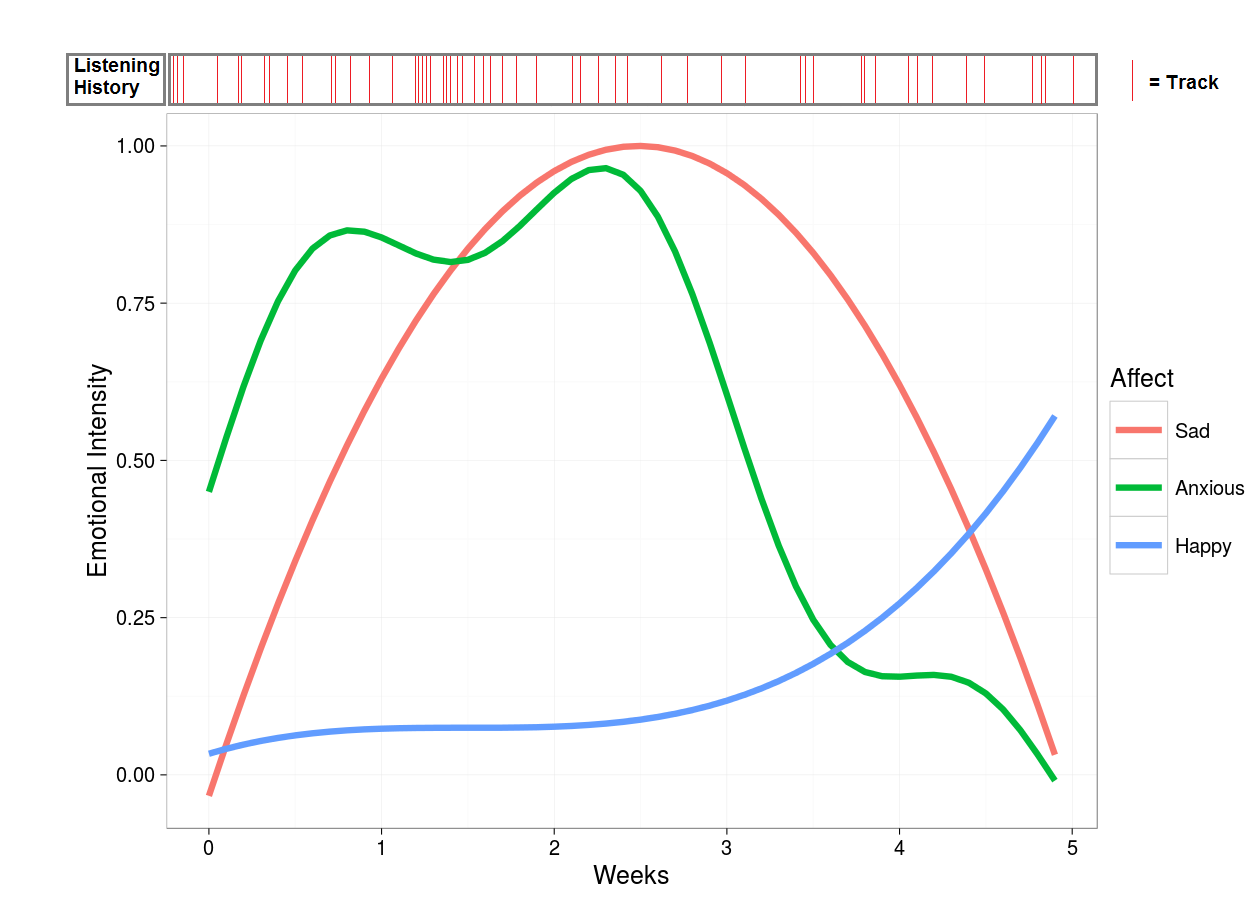
\includegraphics[width=0.8\linewidth]{GRA_mental.png}
\caption[Mental Health and Music]{Graph showing hypothetical data relating to changing affect intensity (y-axis) over time (x-axis). Emotional intensity will be ascertained using NLP, and machine learning classification. Red ticks above the line graph represent date/time of specific tracks in a user's listening history. These data will be mapped to the intensities of the emotion tags.}
\end{figure}



\end{document}
